%%%%Draft version
% \documentclass[12pt,letterpaper,spanish,draft,twoside]{book}
%%%%Final version
\documentclass[12pt,letterpaper,spanish,twoside,final]{book}

\usepackage{Thesis}
% New bibliography system: biber (No bibtex needed)
\usepackage[
  backend=biber
]{biblatex}
\addbibresource{bibliografia.bib}

%%%%For producing modified TOC with less space inbetween.
\usepackage{tocloft}
\setlength\cftparskip{-2pt}
\setlength\cftbeforesecskip{1pt}
\setlength\cftaftertoctitleskip{2pt}

%\includeonly{dedicatoria} %Por debug solo compila un capitulo


\begin{document}

\selectlanguage{spanish}

%%%%Change numbering to alphabetic
%\pagenu⎄mbering{alph}

%%%%Change numbering to roman
\clearpage \pagenumbering{roman}
%\listoftodos

\include{Portada}
\cleardoublepage

\thispagestyle{empty}
\vspace*{8cm}
\begin{flushright}
\textit{Para Onatta\\
por estar siempre en mi corazón.}
\end{flushright}                 

% \newpage
% \thispagestyle{empty}
% \mbox{}

\cleardoublepage

\chapter*{Agradecimientos}

{\small
Agradezco a la Facultad de Estudios Superiores de Acatlán, por ser mi casa durante tantos años y por darme la formación profesional y humana que me acompañará durante toda mi vida.

Agradezco también a la jefatura del programa de Matemáticas Aplicadas y Computación por estar siempre dispuestos a ayudarme y por responder mis dudas de la manera más atenta posible.

Agradezco al Macroproyecto de Tecnologías de Información y la Facultad de Ciencias de la UNAM. En particular, a la UDeSyTI por permitirme utilizar sus instalaciones y por todos los recursos materiales con los que me apoyaron.

A mis sinodales de tesis: Carmen Villar, Francisco Patiño, Jaime Vergara, Victor Palencia y Teresa Carrillo; por todos sus comentarios y correcciones que hicieron de éste un mejor trabajo.

A mi directora de tesis: Carmen Villar; por haberme apoyado mucho más de lo que era su deber durante toda la duración de este trabajo.

Y por supuesto, gracias\ldots

A mis compañeros de MAC, del TKD y de la FES Acatlán en general; por todas las pláticas y momentos compartidos.

A todos mis amigos y familiares, por siempre estar al pendiente de mí.

A mi familia, por apoyarme en todos los retos y proyectos que he emprendido durante toda mi vida.

A Hipatia, por estar a mi lado durante esta reedición de tesis.

A Onatta, por su amor, apoyo y por ser mi alma gemela y compañera de vida. Me complementas y me haces ser una mejor persona siempre.

}

\cleardoublepage

\chapter*{Resumen}
Este trabajo trata de cómo crear una simulación gráfica de un cuerpo flexible.
El cuerpo flexible, está construido --como es costumbre en graficación por computadora-- por una malla tridimensional. Además, en éste trabajo se asume que las aristas de la malla son resortes y que el cuerpo flexible está relleno de aire.

Para hacer una animación basada en Física, se definen un conjunto de fuerzas que actúan sobre los vértices de la malla. Después, se usa la fuerza acumulada para integrar la ecuación de Newton y obtener las velocidades y posiciones de los vértices en la escena.

Las fuerzas aplicadas son: la gravedad, los resortes-amortiguadores y la fuerza de presión. Esta última, es resultado de usar la ecuación del gas ideal.

Se describe a detalle, la creación de un programa que implementa todas estas ideas para hacer una animación interactiva. La implementación se hizo en lenguaje C++ y se usa OpenGL como biblioteca para desplegar gráficos.

Se hacen un conjunto de pruebas para comprobar el correcto comportamiento cualitativo en la implementación. Y por último, se hace un análisis del desempeño del programa; donde se estima que secciones son las computacionalmente más costosas.

Modelado Gráfico de un Cuerpo Neumático con OpenGL a Base de Ecuaciones Diferenciales \textcopyright{} 2008 por Jorge Antonio García Galicia está licenciado bajo Attribution 4.0 International.

Para ver una copia de esta licencia, visite \href{http://creativecommons.org/licenses/by/4.0/}{creativecommons.org/licenses/by/4.0/}

\cleardoublepage
%%%%For changing the title of table of contents
%\renewcommand*\contentsname{}
\tableofcontents
\cleardoublepage
\listoffigures
\cleardoublepage
\listoftables
\cleardoublepage
%\listofalgorithms
%\cleardoublepage


%%%%Change numbering to arabic
\clearpage \pagenumbering{arabic}

\chapter*{Introducción}
\addcontentsline{toc}{chapter}{Introducción}
\markboth{INTRODUCCIÓN}{INTRODUCCIÓN}

Uno de los retos más constantes en las ciencias de la computación, y en especial del área de graficación por computadora, ha sido el de alcanzar cada vez mayor realismo.
Sin embargo, este objetivo comúnmente se opone al de hacer modelos simples que requieran de poco poder de cómputo.

Es cierto que cada vez tenemos computadoras más poderosas, pero como seres humanos que somos siempre hemos querido muchas cosas más de las que tenemos.
Hoy en día el que una simulación se pueda ejecutar rápidamente en una computadora personal es casi tan importante como el que esa simulación se vea real.

Modelos que se sabe son bastante efectivos, como las ecuaciones de Navier-Stokes, también son computacionalmente muy costosos.
Por lo tanto, no pueden ser ocupados en simulaciones que requieren de alcanzar tiempo real.

Los videojuegos son un claro ejemplo de simulaciones que requieren de una adecuada combinación de realismo y rapidez de ejecución.
Dentro de esta área, se dice que se alcanza tiempo real cuando el programa responde más rápido de lo que el usuario puede darle instrucciones.
El objetivo principal de este trabajo es encontrar un modelo que conjunte el mayor realismo posible, sin olvidar alcanzar \emph{tiempo real}.

Hace tiempo, cuando buscaba algún tema interesante para realizar mi trabajo de titulación, no tenía una idea clara de lo que quería hacer.
Por un lado sabía qué me gustaba de las materias de mi licenciatura, también sabía que quería hacer una tesis que de alguna manera tuviera que ver con el área de gráficas por computadora.

Afortunadamente para mi, eso fue lo único que necesité para que la maestra Carmen Villar se interesara en asesorar mi trabajo de titulación, aun cuando no tenía un tema bien definido.
Después de buscar en diversas fuentes de información llegamos al sitio web de Maciej Matyka, sobre simulación basada en física, en donde pude consultar el artículo~\cite{Matyka:Presion}.
Desde el primer momento este artículo llamó  mi atención, el modelo propuesto gozaba de las tres características más deseables en un modelo de simulación: era sencillo de entender, sencillo de implementar y era visualmente muy agradable.

Teníamos entonces una idea de donde comenzar, sólo nos hacía falta un problema que valiera la pena modelar.
Discutiendo en el laboratorio de Linux de la FES Acatlán, quizás un poco inspirados en la película \say{American Beauty}, tuvimos la idea del sistema que dio origen al presente trabajo.
Al final creo que el resultado poco tiene que ver con la inmortal escena, pero estoy convencido de que al menos para mí ha sido un camino igual de inspirador.

Otra meta que quería alcanzar era utilizar Software Libre en todo este trabajo. 
Sin duda, el utilizar una biblioteca como OpenGL me favoreció para poder alcanzar esta meta, al tratarse de una especificación libre y multiplataforma.
La mayor parte del trabajo fue realizada bajo un sistema GNU/Linux y el texto fue escrito en \LaTeX. Considero que este objetivo fue cumplido.

A lo largo del desarrollo, tanto del programa como del trabajo escrito, me encontré con muchísimos obstáculos.
Algunos se debieron a mi desconocimiento de ciertas áreas de la física, y otros simplemente a mi falta de habilidades de programación.
Sin embargo, estoy convencido que en ambos aspectos este trabajo me ayudó a superarme.

La pregunta más importante que ahora trato de responderme es: ¿a quién le sirve este trabajo?
Indudablemente me sirvió a mí el escribirlo, y quiero pensar que también le servirá a cualquier persona que lo lea.
¿Quién puede ser éste lector potencial?
Es un trabajo de animación por computadora, por lo que le debe servir a cualquier persona que desee hacer una animación de cuerpos flexibles.
También creo que es un trabajo que modela adecuadamente las leyes físicas del fenómeno, así que se puede beneficiar de él cualquier persona que desee aprender o enseñar cómo funcionan los cuerpos neumáticos.
Por último, le sirve a cualquier estudiante que busque alguna aplicación de las matemáticas y la física en la animación.

La manera como decidí organizar este trabajo es la siguiente:

En la primera parte se revisó el marco teórico.
Éste trata principalmente de aquellas partes de la literatura, que aunque ya están escritas, quizás no sean tan obvias para estudiantes de la licenciatura de Matemáticas Aplicadas y Computación.
Este capítulo fue por mucho el más divertido de escribir.

En el siguiente capítulo, ya adentrado en la situación a modelar, traté en mayor detalle las estrategias de implementación del modelo.
Es un capítulo en el que intenté plasmar, sobre todo, las cosas que me fueron más difíciles en el desarrollo de la investigación y cómo fue que encontré soluciones a ellas.

El tercer capítulo trata de cómo se hizo el programa en C++ para esta simulación. 
Aunque el código que aquí escribo puede ser mejorado de muchas maneras, es una solución que funciona.
Y si bien no me preocupé en optimizar el código, si se ganó un poco de claridad. 
Además, considero dado el  propósito de este trabajo, que la programación no es \emph{tan} importante.

En el capítulo final, presento las pruebas y juegos a los que sometí mi programa una vez que terminé el desarrollo.
Este capítulo fue por mucho el más gratificante de escribir.
Al escribir este capítulo aprendí dos cosas: que siempre hay más cosas que hacer después de que uno piensa que ha terminado algo y que los resultados no siempre son los que uno espera.
De hecho, el desarrollo de esta investigación, de la que fui parte desde su nacimiento, me hizo llevarme unas cuantas sorpresas en su edad madura.

Por último, sólo me queda esperar que los lectores de este trabajo encuentren al leerlo, un poco de la diversión que me dejó a mí escribirlo.


\chapter{Sistemas físicos y modelación matemática}

\epigraph{\say{In fact, computer graphics is arguably the best example of a practical area where so much mathematics combines so elegantly.}}{\textit{Samuel R. Buss \\ 3-D Computer Graphics A Mathematical Introduction with OpenGL}}

Uno de los principales fenómenos naturales que más se ha estudiado a lo largo de la historia es el del movimiento.
La rama de la física que se encarga de estudiar este fenómeno es la \emph{mecánica}.
Hay muchos enfoques para estudiar el movimiento.
La mecánica puede dividirse a su vez en: \emph{estática}, \emph{cinemática} y en \emph{dinámica}.
La estática estudia la ausencia del movimiento.
La cinética se encarga de estudiar la manera de describir el movimiento.
La dinámica estudia las causas del movimiento, es decir estudia las fuerzas que producen el movimiento.

El movimiento que estamos tratando de modelar puede pensarse como una combinación de movimientos más simples, para los cuales ya existen modelos matemáticos.
Por lo que en este capítulo presentaré estos movimientos por separado, con el fin de entender las causas que los producen.
Después en el capítulo siguiente uniré estos sistemas simples en uno más complejo, que es el que a fin de cuentas nos interesa modelar.

El primer movimiento que presentaré es el de un cuerpo que se deja caer en el vacío sin imprimirle ninguna fuerza, y que por lo tanto, sólo actúa sobre él la fuerza de gravedad.
Este movimiento ha sido muy estudiado y es conocido como \emph{caída libre}. 

El siguiente movimiento, es también muy conocido, se conoce como \emph{ley de Hooke}.
Éste es el movimiento de algunas masas unidas por un resorte y se modela con una ecuación diferencial.

Por último, analizaré el fenómeno de la presión del gas, con el modelo más simple de todos, que es conocido como la ecuación de estado de la \emph{ley de los gases ideales}.
En el cual, se supone un gas hipotético en el que sus moléculas no interactúan entre sí.

En este capítulo, trataré estos sistemas por separado para poder comprenderlos cualitativamente.
Así será más clara la manera en que los combinaré en el siguiente capítulo para formar un modelo.
Y finalmente, con este modelo trabajar la situación que deseo analizar.

\section{Un cuerpo en caída libre}
Imagínese una piedra que descansa cerca de la orilla del quicio de una ventana.
La piedra es empujada horizontalmente hasta que resbala de la orilla y se cae, (ver Figura~\ref{piedra:fig}).
Éste es un ejemplo de caída libre.

Más formalmente, la caída libre consiste en modelar un cuerpo sólido, con masa uniformemente distribuida y despreciando la fricción del aire.
Es decir, la única fuerza que actúa sobre este cuerpo es la \emph{fuerza de gravedad}.

\begin{figure}
 \centering
 \includegraphics[]{img/01/caida_libre}
 \caption[Ejemplo de caída libre]{ 
 Una piedra en caída libre, la única fuerza que actúa sobre ella es la de la gravedad.
 } \label{piedra:fig}
\end{figure}

En la antigüedad, Aristóteles pensaba que este movimiento era directamente proporcional a la masa.
Él afirmaba que dada una misma altura, un cuerpo con el doble de masa caería el doble de rápido.
Esta idea fue aceptada durante varios siglos.
No fue hasta la llegada del método científico que se empezó a cambiar este punto de vista.

Se cuenta una anécdota con ciertos toques de leyenda.
Se dice que Galileo dejó caer en un mismo instante una pelota de madera de un kilo de peso y una bala de cañón de diez kilos de peso desde la torre inclinada de Pisa, y la gente pudo apreciar como estos cayeron casi al mismo tiempo.
Con el simple hecho de un experimento la teoría aristotélica quedaba refutada.
Al parecer antes de los pensadores y filósofos del renacimiento, nadie se había preguntado si los conocimientos que prevalecían eran verdaderos; es decir, nadie había hecho un experimento para probar si algo era de verdad como se decía.
La simple autoridad de Aristóteles bastaba para que se diese por hecho.

Fue después de Galileo en 1685 que Newton explicó con más detalle este movimiento, con su \emph{ley de la gravitación universal}.
Newton fundamentó la mecánica con sus leyes del movimiento y la ley de la gravitación universal.
En las primeras, se dice que un objeto permanece en su estado de reposo o de movimiento rectilíneo uniforme a menos que una fuerza lo perturbe.
Esta fuerza perturbadora le produce al objeto un cambio de velocidad, es decir, una aceleración, en mecánica de Newton las fuerzas producen \emph{aceleración}.
La ley de la gravitación universal dice que todos los cuerpos se atraen.
También dice que la fuerza de atracción entre dos cuerpos es directamente proporcional al producto de sus masas e inversamente proporcional al cuadrado de sus distancias.

A partir de esta idea, si la fuerza cambia con el tiempo, también lo hará la aceleración.
Sin embargo por suerte para nosotros, el movimiento de caída libre imprime siempre \emph{aproximadamente} la misma aceleración, es decir, la fuerza de gravedad actúa sobre todas las cosas con \emph{casi} la misma fuerza.
Una consecuencia de la ley de la gravitación universal y de que la masa de la Tierra sea muy grande en comparación de las cosas que estamos acostumbrados ver caer.

Gracias a que la fuerza que atrae las cosas a la tierra es casi constante, el problema de caída libre tendrá una solución matemática analítica y hasta cierto punto fácil de obtener.
Hay muchas maneras de derivar estas leyes, más adelante cuando se unan todos los modelos se entenderá por qué elegí explicarla de esta manera y no de una manera más natural.

Empiezo planteando las condiciones del modelo: suponemos que se trata de un objeto con masa $m$, que se encuentra al iniciar su movimiento a una altura $y_0$, que en el momento de iniciar su movimiento tiene una velocidad inicial $v_0$ y que durante todo su movimiento sólo va a actuar sobre él una fuerza constante $F$ (Figura~\ref{cida:fig}), que le imprime una aceleración constante $a$ y que esta fuerza es precisamente la fuerza de gravedad que ejerce la tierra sobre él, es decir: $a = g$.

\begin{figure}
 \centering
 \includegraphics[]{img/01/cuerpo_caida}
 \caption[Diagrama de cuerpo libre]{ 
 El modelo del cuerpo en caída libre, con su sistema de coordenadas.
 } \label{cida:fig}
\end{figure}

Además por seguir la convención usual, se moverá en un sistema coordenado derecho, es decir las direcciones positivas serán derecha en el eje $x$, y arriba en el eje $y$, por ende los movimientos hacia abajo y a la izquierda serán negativos, respecto a cada uno de los ejes.
Además sabemos que la gravedad sólo afecta el movimiento vertical del cuerpo, es decir sólo actúa sobre el eje $y$.
Entonces la segunda ley de Newton nos dice que:

\begin{equation} 
F = m a
\end{equation} 

Pero nosotros sabemos que la aceleración $a$, es la derivada de la velocidad $v$, respecto al tiempo $t$.
Y que la velocidad es a su vez la derivada de la posición $y$ respecto al tiempo $t$, por lo que podemos escribir la ley de Newton como:

\begin{equation}
\label{ley:Newton}
 \frac{d^2y}{dt^2} = \frac{1}{m}F(t)
\end{equation}

Además se sabe que tenemos dos condiciones iniciales, para nuestro problema:

$$ y(0) = y_0 $$
$$ v(0) = v_0 $$

Tenemos entonces una ecuación diferencial ordinaria, de segundo orden, con dos condiciones iniciales, por lo tanto podemos encontrar una solución única.

Esta ecuación es en particular, fácil de resolver debido a que la fuerza $F$ es constante.

Primero sabemos que $F(t) = -mg$, el signo es porque la gravedad actúa hacia abajo.
Y sustituyendo en la ecuación:

\begin{equation}
\label{fuerzaGravedad}
\frac{d^2y}{dt^2} = \left(\frac{1}{m}\right)\left( -mg \right) 
\end{equation}

Aquí vemos por qué Galileo encontró que la caída libre \emph{no} depende de la masa del objeto.

Si integramos la ecuación respecto a $t$.

$$ \frac{dy}{dt} = -gt + c_2 $$

Donde $c_2$ es una constante de integración, que puede encontrarse de la primera condición inicial.

$$ \frac{dy}{dt} = -gt + v_0 $$

Podemos volver a integrar la ecuación respecto a $t$ y volver a obtener la nueva constante $c_1$ de las condiciones iniciales.

\begin{eqnarray}
 y(t) & = & -\frac{gt^2}{2} + v_0t + c_1 \nonumber \\
      & = & -\frac{gt^2}{2} + v_0t + y_0
\end{eqnarray}

Que es la función que estábamos buscando, esta función nos dice cual es el valor de la coordenada $y$ del objeto cuando ha transcurrido un tiempo $t$.
Esto es precisamente lo que necesitamos saber para hacer una animación: una función que nos diga cómo se mueve algo conforme pasa el tiempo.
También cabe señalar que en nuestro caso de la caída libre $v_0 = 0$, recordemos que el cuerpo se dejó caer, por lo que nuestra función se simplifica.
Y se puede simplificar aún más, si escogemos un sistema de referencia tal que el movimiento del objeto empiece en el origen de dicho sistema es decir $y_0 = 0$.
La forma más simple de nuestra función es entonces:

\begin{equation}
 y(t) = -\frac{gt^2}{2}
\end{equation}

Quizás este sistema puede parecer un poco simple, y en efecto lo es, en el sentido que pudo resolverse sin mayor problema y de una manera analítica, esto se debió a que la aceleración, y por ende la fuerza se supuso constante.
El valor de este modelo radica más bien en la existencia de una solución analítica.

\section{El sistema masa-resorte}

Para explicar esta situación se partirá desde lo más simple a lo más complejo.
El modelo más sencillo se conoce como un \emph{oscilador armónico simple}.
Después se tratará de agregar una segunda fuerza que servirá como un amortiguador, este nuevo modelo se conoce como \emph{oscilador armónico amortiguado}.
Por último este modelo se generalizará a un sistema en tres dimensiones y con vectores y finalmente derivaremos la fórmula que ocuparemos durante el resto del trabajo. 

La mecánica de vibraciones se debe al físico inglés Robert Hooke, la vida de este científico es muy interesante por diversos motivos.\footnote{Una biografía de Hooke se puede encontrar en la \href{https://es.wikipedia.org/wiki/Robert_Hooke}{wikipedia} en español; una biografía aun más completa, en \href{https://mathshistory.st-andrews.ac.uk/Biographies/Hooke/}{MacTutor}}
Es uno de los científicos experimentales más importantes de la historia,  y sus estudios abarcan campos muy diversos como la biología, la medicina, la cronometría, la física planetaria, la microscopía, la náutica y la arquitectura. 
Estuvo en disputas con Newton por el descubrimiento de la ley de la gravitación universal.

Aquí estamos interesados en uno de sus descubrimientos en elasticidad y que es conocido como \emph{Ley de Hooke}.
Que nos dice: 
\begin{quote}
La fuerza restauradora ejercida por un resorte es linealmente proporcional al desplazamiento del resorte desde su posición de reposo y está dirigida hacia esa misma posición\footnote{En el libro~\cite{Blanchard:Ecuaciones} en el apartado dedicado a Modelación por medio de Sistemas, se enuncia de esta manera, ignoro si Hooke pensó en resortes al enunciar su ley, o se le descubrió esta aplicación en un momento posterior.}.
\end{quote}

\subsection{Oscilador armónico simple}
Imagínese que se tiene una masa sujeta por un resorte sobre la que no actúa ninguna fuerza adicional.
Por el momento vamos a suponer que no hay fricción del medio, presumiblemente el aire y que no está sujeta a la fuerza de gravedad.
Por estas condiciones ideales la masa no tendrá pérdida de energía, es decir se moverá por siempre.

De nuevo la misma idea que antes; ocuparemos la ecuación de Newton y lo único que cambiará en nuestro modelo será la expresión para calcular la fuerza, en vez de la fuerza de gravedad, se modelará la fuerza del resorte.

Imaginemos el resorte; los resortes se estiran y se comprimen cuando se les aplica una fuerza.
Siempre que pasa esto, el resorte en respuesta ejerce una fuerza restauradora, esta fuerza siempre lucha por devolver al resorte a su punto original de reposo es decir a donde no está ni comprimido ni estirado.
Es entonces que la ley de Hooke para los resortes nos da una manera de calcular esta fuerza restauradora $F_s$.

Empecemos a plantear las condiciones del modelo, supongamos que es una masa unida por un resorte a un objeto inamovible, una pared por ejemplo y que todo el sistema descansa en el piso, para que no lo afecte la gravedad, y este piso no le da ningún tipo de fricción.
En estas condiciones el único movimiento permitido para la masa será el horizontal y a la derecha, de nuevo por convención diremos que es a la dirección positiva del eje $x$.
La Figura~\ref{masaResorte:fig} ilustra la situación aquí descrita.

\begin{figure}[htb]
 \centering
 \includegraphics[width=0.6\textwidth]{img/01/masaResorte}
 \caption[Masa unida por un resorte]{ 
 Una masa que se mueve solamente afectada por la fuerza de un resorte.
 } \label{masaResorte:fig}
\end{figure}

Se trata de modelar el movimiento de la masa a lo largo del tiempo $t$.
La masa del cuerpo de nuevo la denotaremos como $m$ y el origen del sistema será el punto donde el resorte se une a la pared.
Supongamos también que cuando el resorte está en reposo tiene un largo $L$.
La expresión que nos dice cual es la fuerza del resorte, que denotaremos como ya se dijo $F_s$, para un estiramiento razonablemente pequeño es la \emph{ley de Hooke para los resortes} y se escribe como sigue:

\begin{equation}
F_s = -k_s \left( x - L \right)
\end{equation}

Esta expresión básicamente nos dice que la fuerza es proporcional a la distancia de la masa a su punto de equilibrio donde el resorte está en reposo.
La nomenclatura $F_s$ se debe a que la mayoría de la bibliografía consultada está en inglés y traté de ser consistente con ella, ésta es la fuerza del resorte o \emph{\textenglish{spring force}}.

Se observa en esta expresión que cuando el resorte está estirado, es decir, su largo $x$ es mayor a $L$ la fuerza del resorte se vuelve negativa y por ende jala a la masa a su punto de reposo.
Como se ve en la Figura~\ref{fig:estirada}.

\begin{figure}
 \centering
  \begin{subfigure}[b]{0.5\textwidth}
    \includegraphics[width=\textwidth]{img/01/masaEstirada}
    \caption{Cuando $x>L$, el resorte jala la masa.}
  \label{fig:estirada}
  \end{subfigure}
\\
  \begin{subfigure}[b]{0.5\textwidth}
    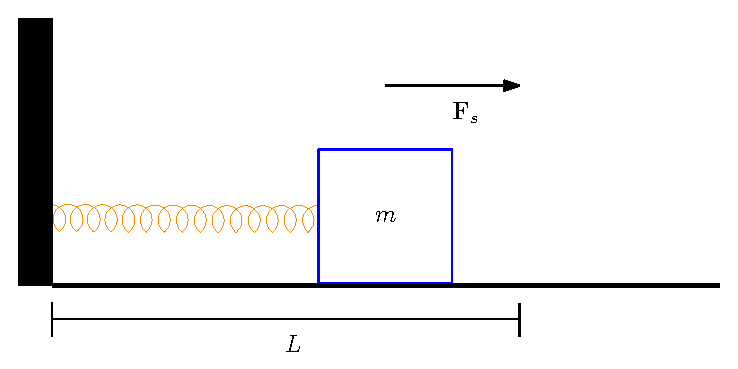
\includegraphics[width=\textwidth]{img/01/masaCompresa}
    \caption{Cuando $x<L$, el resorte empuja la masa}
    \label{fig:compresa}
  \end{subfigure}
 \caption[Ley de Hooke para resortes]{ 
 $F_s$ trata de llevar el sistema a $x = L$
 } \label{leyHokke:fig}
\end{figure}

En el caso que el resorte esté compreso (Figura~\ref{fig:compresa}), es decir, $ x < L$, el resorte empuja el cuerpo para que alcance la posición de reposo y de nuevo lo hace con una fuerza proporcional a la distancia que esté alejado del cuerpo de este punto. 

También se observa que cuando el largo del resorte es $ x = L$ el resorte está en reposo y por lo tanto la fuerza se hace cero, éste es el caso que se ilustró en la Figura~\ref{masaResorte:fig}.

Esta expresión para la fuerza se vuelve a aplicar a la ecuación de la ley de Newton, quedando la siguiente ecuación diferencial.

\begin{eqnarray}
m \frac{d^2x}{dt^2} & = & F(t) \nonumber \\
                    & = & F_s \nonumber \\
                    & = & -k_s \left( x - L \right) \nonumber \\
\frac{d^2x}{dt^2} + \frac{k_s}{m}x  & = & \frac{k_s L}{m}
\end{eqnarray}

Esta ecuación de nuevo tendrá solución única si se especifican un par de condiciones iniciales de la forma $x(0) = x_0$ y $ v(0) = v_0 $.
La teoría de ecuaciones diferenciales nos dice que esta solución se puede encontrar, mediante la suma de una solución particular $x_p$ y una solución general de la ecuación diferencial homogénea asociada al problema $x_h$.
Es decir $x(t) = x_p + x_h$.

Por simple inspección se puede ver que $x(t)= L$ es una solución que nos puede servir como $x_p$ y afortunadamente la ecuación homogénea  es una \emph{ecuación diferencial lineal ordinaria de coeficientes constantes} por lo que es relativamente simple de resolver.
Además recuérdese que las constantes $k_s$, $m$ y $L$, son todas positivas por lo que una solución es:

\begin{equation}
x_h = c_1 \cos{\sqrt{\frac{k_s}{m}}}t + c_2 \sin{\sqrt{\frac{k_s}{m}}}t
\end{equation}

Con estas dos soluciones tenemos:
\begin{eqnarray}
x(t) & = & x_p + x_h \nonumber \\
     & = & c_1 \cos{\left(\sqrt{\frac{k_s}{m}} t \right)} + c_2 \sin{\left(\sqrt{\frac{k_s}{m}} t \right)} + L
\end{eqnarray}

Y podemos determinar las dos constantes de integración $c_1$ y $c_2$ de las condiciones iniciales.

Para este problema en particular la solución que estamos buscando es:

\begin{equation}
x(t) = \left(x_0 - L \right) \cos{\left(\sqrt{\frac{k_s}{m}} t \right)} +  \left( v_0 \sqrt{\frac{m}{k_s}}\right) \sin{\left(\sqrt{\frac{k_s}{m}} t \right)} + L
\end{equation}

Como puede apreciarse en la solución el cuerpo nunca deja de moverse, su movimiento está expresado por una función periódica.
Esto es debido a que en un medio ideal como éste el sistema no disipa energía por lo tanto, nunca cesa su movimiento, y el resorte se comprime y se estira de la misma manera por siempre.

\subsection{Oscilador armónico amortiguado}

Como es lógico las condiciones ideales antes tratadas son casi imposibles de alcanzar en la realidad, por lo que es necesario agregar a nuestro sistema una manera de perder energía.

Una manera simple de hacerlo es agregándole una resistencia por parte del medio, por ejemplo el aire, o el agua si todo el sistema se ha sumergido bajo ésta. 

Esta nueva fuerza en el sistema, a menudo se supone directamente proporcional a la velocidad del cuerpo con respecto al medio en el que se encuentra y se modela con la siguiente ecuación.

\begin{equation}
F_d = -k_d\frac{dx}{dt}
\end{equation}

El signo es negativo debido a que la resistencia del medio se opone a la velocidad. Es decir trata de detener la masa poco a poco.
De nuevo una aclaración sobre la nomenclatura: se dice que está es la fuerza de amortiguación y se refiere a la palabra amortiguador en inglés: \emph{\textenglish{damping}}.
Y entonces el nuevo modelo toma la forma:

\begin{eqnarray}
m \frac{d^2x}{dt^2} & = & F_s + F_d \nonumber \\
& = & -k_s \left( x - L \right) -k_d\frac{dx}{dt} \nonumber \\
m \frac{d^2x}{dt^2} + k_d\frac{dx}{dt} + k_s x & = & k_s L 
\end{eqnarray}
Una vez más sujeto a las mismas condiciones iniciales $x(0) = x_0$ y $ v(0) = v_0$.

Esta ecuación se resuelve de una manera similar a la de la sección pasada, donde una solución particular $x_p$ vuelve a ser $x_p = L$.
Para encontrar una solución general se requiere resolver la ecuación homogénea asociada:

\begin{equation}
m \frac{d^2x}{dt^2} + k_d\frac{dx}{dt} + k_s x = 0
\end{equation}

De nuevo la teoría nos dice que esta ecuación tiene una solución de la forma:

\begin{equation}
x(t) = c_1 e^{n_1 x} + c_2 e^{n_2 x} \nonumber
\end{equation}

Donde las constantes $n_1$ y $n_2$ son soluciones de la ecuación algebraica en $n$:

\begin{equation}
m n^2 +  k_d n + k_s = 0
\end{equation}

Dado que ésta es una ecuación de segundo grado, puede resolverse con la fórmula general.
Además se puede obtener información de la solución analizando cómo es $k_d^2$ con respecto a $4 m k_s$ (lo que vendría a ser $b^2$ con respecto a $4ac$).
Esto nos lleva a tres casos: que $n$ tenga dos valores reales diferentes, que $n$ tenga un solo valor real y que $n$ tenga un par de valores complejos conjugados.

Estos casos son analizados a detalle en~\cite{Ross:Ecuaciones} y por lo tanto lo único que diré es que los dos primeros casos nos llevan a resultados donde el amortiguador es tan fuerte que no deja a la masa oscilar ni siquiera una vez.
Es decir en donde la fuerza del medio es muy superior a la fuerza del resorte.

El único caso que a nosotros nos interesa es precisamente aquel donde el amortiguador es débil, y deja oscilar a la masa unas cuantas veces antes de detenerla, este caso se da precisamente cuando se trata de dos valores complejos conjugados de $n$. 

Este caso es cuando $k_d^2 < 4 m k_s$ es decir que el discriminante de la ecuación es negativo, por lo que la solución es de la forma:
\begin{eqnarray}
n_1 & = & \alpha + \beta i \nonumber \\
n_2 & = & \alpha - \beta i \nonumber
\end{eqnarray}
En donde:
\begin{eqnarray}
\alpha & = & \frac{k_d}{2m} \nonumber \\
\beta  & = & \frac{\sqrt{4 m k_s - k_d^2}}{2m} \nonumber
\end{eqnarray}
Y por tanto la ecuación diferencial tiene una solución de la forma:

\begin{equation}
\label{solOsiArmAmor} 
x(t) = e^{-\alpha t} \left( c_1 \cos{\beta t} + c_2 \sin{\beta t} \right) + L
\end{equation}

De nuevo por medio de las condiciones iniciales se pueden obtener los valores de las constantes $c_1$ y $c_2$, quedando de esta manera:

\begin{eqnarray}
c_1 & = & x_0 - L \nonumber \\
c_2 & = & \frac{v_0 + \left( x_0 - L \right) \alpha }{\beta } \nonumber 
\end{eqnarray}

De la solución \eqref{solOsiArmAmor} es claro que cuando el tiempo $t \rightarrow \infty $, el factor $e^{-\alpha t}$ dominará y la masa se detendrá poco a poco.

A manera de ejemplo ilustrativo, podemos elegir un conjunto arbitrario de valores para los parámetros. 
Por ejemplo, si $m = \frac{1}{2}$, $k_d = \frac{1}{10}$, $k_s = \frac{1 + 1 / 100}{2} = 0.505$, $L = 3$, $x_0 = 6$ y $v_0 = 3 - 3/10 = 2.7$.
Entonces $\alpha = \frac{1}{10}$, $\beta = 1$, $c_1 = 3$ y $c_2 = 3$.
Lo que conduce a la solución $x(t) = e^{\frac{-1}{10}t} \left( 3 \cos{t} + 3 \sin{t} \right) + 3$, cuyo comportamiento se puede ver en la Figura~\ref{OsciAmor:fig}.

\begin{figure}[htb]
 \centering
 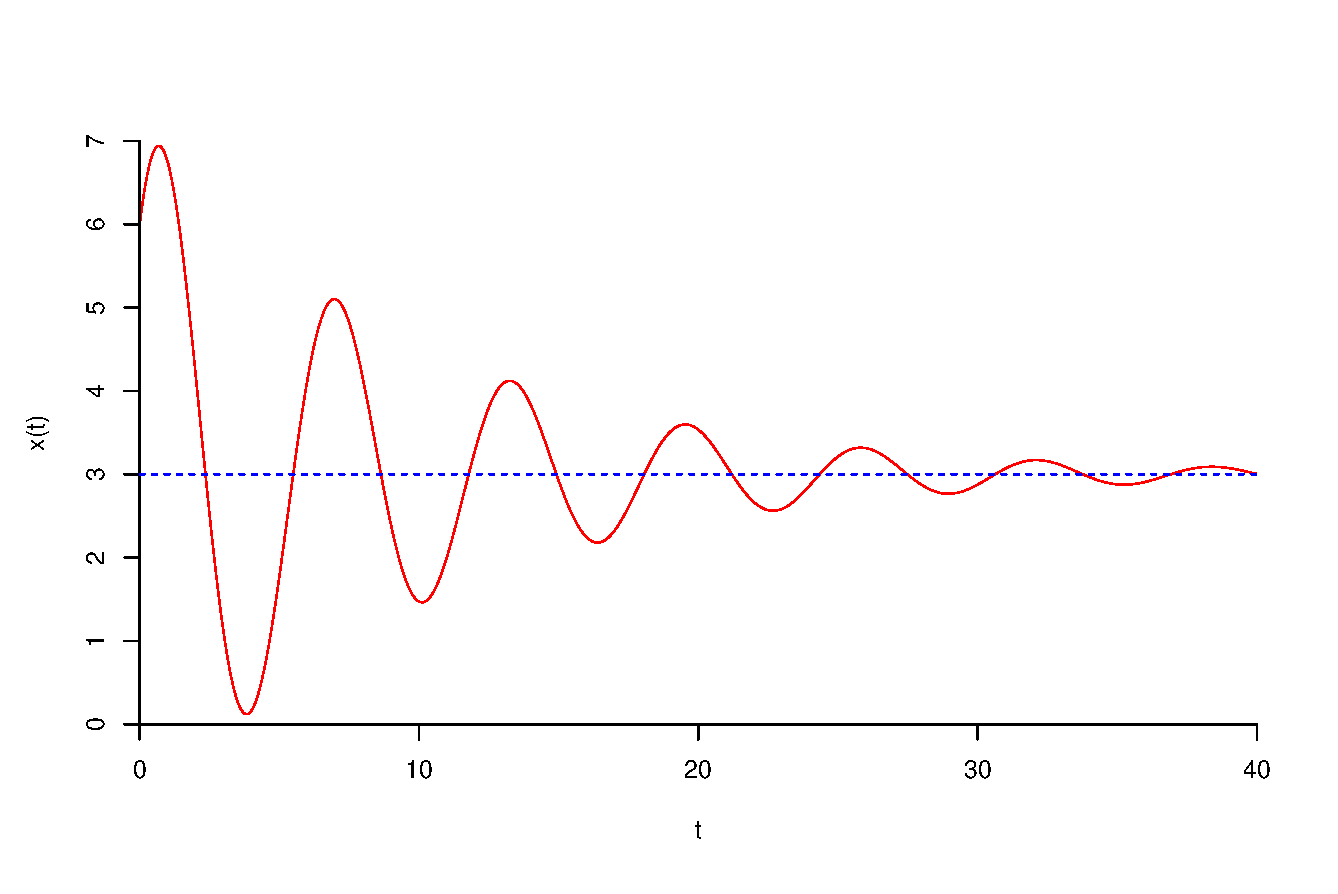
\includegraphics[width=0.85\textwidth]{img/01/oscilador_amortiguado}
 \caption[Plano fase del oscilador armónico amortiguado]{ 
 Gráfica de $x(t) = e^{\frac{-1}{10}t} \left( 3 \cos{t} + 3 \sin{t} \right) + 3$. La línea discontinua en azul indica el estado de equilibrio: $x(t) = L$.
 } \label{OsciAmor:fig}
\end{figure}

\subsection{Masa-resorte en más de una dimensión}

Tomaremos el modelo de la sección anterior; pero lo vamos a generalizar de manera que se pueda modelar este mismo fenómeno unidimensional solo que situado en un espacio tridimensional.
Por medios geométricos trataré de aplicar las mismas fórmulas de la sección pasada.
Por simplicidad en los diagramas, voy a explicar el caso de dos dimensiones, sin embargo, como la explicación se hará con vectores, no se debe de tener problema en generalizar para tres dimensiones.

De aquí en adelante, para la notación matemática; usaré la convención de escribir los vectores en negritas y los escalares en fuente normal~\footnote{Ésta es una convención muy aceptada en la literatura de las gráficas por computadora}.

Primero vamos a considerar que hay dos puntos en el espacio que están unidos por un resorte, este resorte es la única fuerza que actúa sobre ellos.
El resorte no tiene masa y ambos cuerpos tienen una masa $m$.
Los puntos no están sujetos, es decir se mueven libremente por el espacio, y la única fuerza que actúa sobre ellos es el resorte.

Hay que notar que a diferencia de la sección pasada, donde el resorte estaba empotrado en la pared, aquí el resorte está unido a dos puntos sueltos, y por lo tanto aplica la misma fuerza sobre cada uno de los puntos.
Esto se puede apreciar mejor en la Figura \ref{masaSuelta:fig}.

\begin{figure}[hbt]
\centering
  \begin{subfigure}[b]{0.45\textwidth}
    \includegraphics[width=\textwidth]{img/01/resortesJuntos}
    \caption{Cuando $\textbf{r}<L$, el resorte empuja ambas masas}
    \label{fig:juntos}
  \end{subfigure}
\\
  \begin{subfigure}[b]{0.5\textwidth}
    \includegraphics[width=\textwidth]{img/01/resortesNormal}
    \caption{Cuando $\textbf{r}=L$, el resorte no ejerce fuerza}
    \label{fig:normales}
  \end{subfigure}
\\
  \begin{subfigure}[b]{0.7\textwidth}
    \includegraphics[width=\textwidth]{img/01/resortesSeparados}
    \caption{Cuando $\textbf{r}>L$, el resorte jala ambas masas.}
    \label{fig:estirados}
  \end{subfigure}
 \caption[Masas libres en el espacio unidas por un resorte]{ 
 Como las masas están libres, el resorte aplica sobre cada una de ellas la misma fuerza, pero en sentido contrario.
 } \label{masaSuelta:fig}
\end{figure}

Llamaré estos puntos $a$ y $b$ respectivamente, y vemos que una posible manera de localizarlos en el espacio es el vector de posición de cada uno de ellos, denotados por $\textbf{p}_a$ y $\textbf{p}_b$.

\begin{figure}
 \centering
    \includegraphics[width=7cm]{img/01/vector_posicion}
 \caption[Ejemplo de vectores de posición]{ 
 Podemos localizar puntos en el espacio por medio de sus vectores de posición.
 } \label{posVec:fig}
\end{figure}

\subsubsection{La fuerza del resorte}

Vamos a calcular la fuerza del resorte sobre el punto $a$; la denotaré como $\textbf{F}_a$, y por lo anterior ya se sabe que la fuerza que actúa sobre $b$ es su negativo, es decir $\textbf{F}_b = -\textbf{F}_a$

Sabemos que una manera de encontrar el vector que une los puntos $a$ y $b$ es restando los vectores de posición de cada uno de ellos; a este nuevo vector lo llamaremos $\textbf{r}$ así que:

\begin{equation}
\textbf{r} = \textbf{p}_a - \textbf{p}_b
\end{equation}

Como se ve en la Figura~\ref{posVec:fig} este vector empieza en la punta de $\textbf{p}_b$ y termina en la punta de $\textbf{p}_a$.
Entonces la distancia que hay de $a$ a $b$ es precisamente la norma de este vector $\textbf{r}$, dicho de otra manera $\textbf{r} = \textbf{p}_a - \textbf{p}_b$ y $\overline{ab} = |\textbf{r}|$.

Ahora que sabemos la distancia de $a$ a $b$, la podemos restar con el tamaño de resorte que es el escalar $L$.
Si a este resultado lo multiplicamos por la constante del resorte $k_s$ sabremos la magnitud de la fuerza del resorte, es decir calculando $k_s \left( |\textbf{r}| - L \right)$.

Éste es un escalar, que representa la magnitud de la fuerza, pero como ésta última es un vector, hace falta que le demos dirección, para hacerlo multiplico el escalar por el vector $\textbf{r}$ normalizado.

Analizaremos la acción de la fuerza.
Si el factor $k_s \left( |\textbf{r}| - L \right)$ es negativo, entonces $| \textbf{r} | < L$, significa que el resorte está comprimido, luego entonces la fuerza debe empujar el punto $a$ lejos del punto $b$, como ya dijimos que $\textbf{r}$ representa un vector que va de $b$ a $a$, entonces la fuerza debe tener la dirección de este vector.
Veamos el caso contrario, si $ | \textbf{r} | > L $ el resorte está estirado, $k_s \left( |\textbf{r}| - L \right)$ es positivo y la fuerza debe jalar el punto $a$ en dirección de $b$, es decir en la dirección contraria que el vector $\textbf{r}$.
De estas dos observaciones nos damos cuenta de que el signo de $k_s \left( |\textbf{r}| - L \right)$ debe ser negativo, es decir:

\begin{equation}
\label{fuerza:resorte}
\textbf{F}_a = -k_s \left( |\textbf{r}| - L \right) \frac{\textbf{r}}{|\textbf{r}|}
\end{equation}

Como se dijo, sólo se ha calculado la fuerza que actúa sobre el punto $a$, sin embargo por la simetría del sistema y que ambos puntos están sueltos en el espacio, la fuerza sobre el punto $b$, es equivalente pero en sentido contrario, es decir:
$$ \textbf{F}_b = - \textbf{F}_a $$

\subsubsection{La fuerza del amortiguador}

En la sección pasada sólo modelamos la fuerza de un resorte que en esencia presenta la misma carencia del primer resorte que analizamos: le falta una manera de perder energía.
Ya habíamos analizado una manera eficaz de hacer que el oscilador disipe energía, sin embargo esto se debía al medio.
Aquí la idea es un poco diferente, vamos a pensar que esta resistencia no está presente en el medio, sino en el mismo resorte en sí; es decir nuestro resorte además de ser tal será un amortiguador, y la resistencia actuará por lo tanto en la misma línea de acción del resorte.

Ya dijimos anteriormente que esta resistencia la vamos a suponer proporcional a la velocidad.
Y con la misma idea que antes vamos a agregarla al modelo anterior.
Ya sabemos que tenemos una manera de localizar a los puntos $a$ y $b$ en el espacio, su vector de posición, sin embargo aún no tenemos una manera de saber la velocidad de los puntos en el espacio, por ello vamos a crear dos vectores $\textbf{v}_a$ y $\textbf{v}_b$, que contienen la velocidad a la que se mueven estos puntos respectivamente.

Procedamos a calcular la fuerza que actúa sobre el punto $a$.
Estas fuerzas son: la fuerza anterior debida al resorte que los une, y una nueva fuerza ahora debida al amortiguador.

\begin{equation}
\textbf{F}_a = \textbf{F}_s + \textbf{F}_d
\end{equation}

Donde $\textbf{F}_s$ es precisamente la expresión \eqref{fuerza:resorte}. Así que sólo nos falta calcular $\textbf{F}_d$.
Esta fuerza, como ya se dijo, es proporcional a la velocidad a la que se mueve un punto respecto al otro $\left( \textbf{v}_a - \textbf{v}_b \right)$ con una constante $k_d$, y además actúa en el sentido contrario al de la velocidad, es decir $F_d$ es proporcional a $-k_d \left( \textbf{v}_a - \textbf{v}_b \right)$.


Ahora hay que notar también que la posición de un punto no necesariamente tiene que ver con su velocidad, es decir un punto en una misma posición se podría mover bien a una velocidad $\textbf{v}$ u a otra muy diferente, sin tener que cambiar su vector de posición.

Como ya dijimos que para nosotros el amortiguador está en el resorte, es necesario entonces trasladar esta fuerza a donde está el resorte, es decir a $\textbf{r} = \textbf{p}_a - \textbf{p}_b$.
Para hacer esto vamos a ocupar la conocida forma de la proyección de un vector sobre otro.

Sabemos que un vector $\textbf{A}$ se puede proyectar sobre un vector $\textbf{B}$ y se denota como $\mathrm{Proy}_{ \textbf{B} } \textbf{A}$ podemos obtener su magnitud con la siguiente fórmula:

\begin{equation}
| \mathrm{Proy}_{\textbf{B}} \textbf{A} | = \frac{ \textbf{A} \cdot \textbf{B} }{| \textbf{B} |}
\end{equation}

Ahora entonces calculemos la magnitud de la proyección del vector $\left( \textbf{v}_a - \textbf{v}_b \right)$ sobre el vector donde está el resorte, es decir sobre el vector $\textbf{r} = \textbf{p}_a - \textbf{p}_b$.
Quedando de esta manera:

\begin{equation}
 | \mathrm{Proy}_{ \textbf{r} } \textbf{v} | = \left[ \frac{ ( \textbf{v}_a - \textbf{v}_b ) \cdot ( \textbf{p}_a - \textbf{p}_b ) }{ | \textbf{p}_a - \textbf{p}_b | } \right]
\end{equation}

Sin embargo, esta cantidad es un escalar así que necesitamos multiplicarla por un vector unitario para darle dirección.
Como esta fuerza es debida al \emph{resorte-amortiguador} y está en su misma línea de acción, la multiplicamos por $\textbf{r}$ normalizado.
Quedando la expresión final para $\textbf{F}_d$:

\begin{equation}
\textbf{F}_d = - k_d \left[ \frac{ ( \textbf{v}_a - \textbf{v}_b ) \cdot ( \textbf{p}_a - \textbf{p}_b ) } { | \textbf{p}_a - \textbf{p}_b |} \right] \left[ \frac{ \textbf{p}_a - \textbf{p}_b } { | \textbf{p}_a - \textbf{p}_b |} \right]
\end{equation}

Como ya expliqué antes ésta es sólo la fuerza del amortiguador así que la expresión de fuerza para este \emph{resorte-amortiguador} (remplazando $\textbf{r} = \textbf{p}_a - \textbf{p}_b$ y $\textbf{v} = \textbf{v}_a - \textbf{v}_b$ para no hacer muy compleja la notación) es la siguiente:

\begin{eqnarray}
\textbf{F}_a & = & \textbf{F}_s + \textbf{F}_d \nonumber \\
\textbf{F}_a & = & -k_s \left( |\textbf{r}| - L \right) \frac{\textbf{r}}{|\textbf{r}|} - k_d \left[ \frac{ \textbf{v} \cdot \textbf{r} }{ |\textbf{r}|} \right] \left[ \frac{\textbf{r}} {|\textbf{r}|}\right] \nonumber \\
\label{fuerzaResorte}
\textbf{F}_a & = & - \left\{ k_s \left( |\textbf{r}| - L \right) + k_d \left[ \frac{ \textbf{v} \cdot \textbf{r} }{ |\textbf{r}|} \right] \right\} \left[ \frac{\textbf{r}} {|\textbf{r}|} \right] \\
\textbf{F}_b & = & -\textbf{F}_a \nonumber
\end{eqnarray}

\section{El modelo del gas ideal}

Aquí se va a tratar de agregar al modelo, una fuerza de presión.
La idea de esta fuerza es tomada del artículo de Matika \cite{Matyka:Presion}, y se basa en implementar un modelo simple de gas.
Este modelo cuenta con la ventaja de la sencillez, tanto en su implementación como en la rapidez de su ejecución, lo que lo hace un modelo ideal para una animación en tiempo real.

Vamos a empezar por imaginar un cuerpo cerrado en tres dimensiones, por ejemplo una esfera o un cubo, luego vamos a imaginar que la envolvente de ese cuerpo, es decir la superficie que lo cierra, es una superficie elástica, que se puede estirar y deformar, y por último supongamos que dentro de ese cuerpo, en vez de haber un vacío, hay un gas; ésta es la idea principal del modelo que trataremos de ahora en adelante, y es el motivo de estudio de este trabajo.

En las dos secciones anteriores hemos tratado los modelos que nos pueden servir como la envolvente de este cuerpo (podría ser una envolvente formada por una membrana de puntos unidos por resortes), pero hablaré más de esto en el siguiente capítulo.
Así que sólo falta tratar el modelo de un gas por separado, para terminar nuestro tratamiento de modelos simples.
El modelo que vamos a estudiar es el del \emph{gas ideal}.

\subsection{La termodinámica}

Habíamos estado hablando de leyes de mecánica, sin embargo este modelo pertenece a una rama diferente de la física, la \emph{termodinámica}.
La termodinámica es la rama de la física que estudia los efectos de los cambios de temperatura, calor y presión, en un sistema, por medio de métodos estadísticos.\footnote{En esta definición de \emph{termodinámica} comúnmente se aplican modelos más complejos que el usado aquí, que sí requieren de métodos estadísticos, pero de hecho nuestro modelo es en esencia determinista.}

El estudio de la termodinámica empieza con el descubrimiento de las maneras de medir el calor, es decir, con la invención de los primeros termómetros, fue así como se notó que existen sistemas que presentan cambios cualitativos, cuando cambian su temperatura.

Uno de estos sistemas es el gas, y por lo tanto existen algunos modelos para estudiar las propiedades de los gases.
El más simple de estos modelos es el modelo del gas ideal, que se define por medio de la \emph{ley de los gases ideales}, que no es otra cosa que la ecuación de estado de un gas ideal.

\subsection{Un modelo simple}

Al principio, para poder estudiar un fenómeno del cual no se conocen muchas cosas, es común relajar muchas de sus propiedades e idealizar muchas situaciones, es decir construir modelos simples, en este caso nos abocamos al primer modelo que se construyó para un gas, y por lo mismo está sujeto a muchas suposiciones que en la realidad nunca son alcanzadas por ningún gas, de ahí que lo llamaran \emph{gas ideal}.

En física y en química, una ecuación de estado es una ecuación que describe el estado de agregación de la materia en función de ciertos parámetros, es decir determina la relación matemática entre dos o más funciones de estado asociadas con la materia.

En nuestro caso queremos describir el estado de un gas en función de propiedades macroscópicas del mismo.
Estas propiedades son: la temperatura, el volumen, la presión y el número de moléculas.

Por medio de resultados experimentales se determinó la primera ecuación de estado, una explicación de cómo se hicieron estos experimentos y se llegó a ella se puede encontrar en~\cite{Resnick:Fisica}, pero a nosotros nos bastará con conocerla:

\begin{eqnarray}
PV & = & nRT \nonumber \\
P & = & \frac{1}{V}nRT
\end{eqnarray}

En donde $P$ es la presión del gas, $V$ es el volumen del gas, $n$ es el número de moles, $R$ es una constante llamada constante del gas ideal y $T$ es la temperatura.
La constante $R$ es la multiplicación de la constante de Boltzman y el número de Avogadro~\footnote{Esta constante universal aparece en varias ecuaciones importantes de la termodinámica, es equivalente a la constante de Boltzman pero expresada en unidades de energia.}.
Las unidades de esta constante son Joule ($J$) sobre mol ($mol$) Kelvin ($K$).

$$ R = N_A k = 8.3145 \ \frac{J}{mol \cdot K}$$

Esta ecuación de estado es un aproximación bastante buena cuando se trata de gases a bajas densidades, y la experimentación nos muestra que en estas condiciones \emph{todos} los gases tienden a comportarse como este gas ideal.

\subsection{La presión de un gas}

La presión no es en sí una fuerza sino es una fuerza aplicada en una unidad de área, y por eso se mide en una unidad llamada \emph{Pascals} (Pa) y no en Newtons (N) que es la unidad en que se mide la fuerza.
Entonces, si $\textbf{P}$ es la presión, $\textbf{F}$ es una fuerza y $A$ el área donde se está aplicando esta fuerza:

$$ \textbf{P} = \frac{\textbf{F}}{A} $$

De tal manera que si nosotros queremos una \emph{fuerza de presión}, para poder acumularla en la ecuación de Newton; como lo hicimos con las fuerzas anteriores necesitamos multiplicarla por el área de aplicación.
Dicho de otra manera:

$$ \textbf{F}_p = \textbf{P} \cdot A $$

Donde $\textbf{F}_p$ es la fuerza de presión que estamos buscando, $A$ es el área de aplicación y $\textbf{P}$ es el vector que representa la presión.
Ya se dijo que la magnitud de la presión puede calcularse con la ecuación de estado, pero no se ha dicho qué dirección lleva.
La presión actúa sobre la superficie de la cara del cuerpo, y es siempre de normal a esta cara, de manera que la presión es:

$$ \textbf{P} = P \cdot \textbf{n} $$

En donde $P$ es el escalar calculado con la ecuación de estado y $\textbf{n}$ es un vector unitario normal a la cara sobre la que se está calculando la presión.

Para nuestro modelo se debe tomar en cuenta que sólo nos interesa calcular la fuerza de presión, de esta manera se procede de la siguiente manera.

$$ P = \frac{1}{V} \; nRT $$

De esta manera $\textbf{P}$ es:

$$ \textbf{P} = \frac{1}{V} \; nRT \left[ \textbf{n} \right] $$

Y este vector $\textbf{P}$ se usará a su vez, para obtener el vector fuerza, es decir:

$$ \textbf{F}_p = \frac{1}{V} \; nRT \left[ \textbf{n} \right] A $$

Reacomodando esta ecuación, se tiene:

$$ \textbf{F}_p = \left[ \frac{1}{V}A \; nRT \right] \textbf{n} $$

Donde para \emph{nuestro} modelo el escalar $nRT$ es un parámetro a determinarse experimentalmente, está formado por la temperatura que consideramos constante, el número molar del gas, que debe depender del gas y por la constante del gas ideal. 
Así que los tres son agrupados en una sola constante, que nosotros por ser consistentes con nuestra nomenclatura llamaremos $k_g$

De manera que: 

\begin{equation}
\label{fuerzaGas}
\textbf{F}_p = \left[ \frac{1}{V}A \; k_g \right] \textbf{n}
\end{equation}

Donde $\textbf{F}_p$ es la fuerza que deseamos acumular en cada partícula, $V$ es el volumen total de nuestro cuerpo cerrado, $A$ es el área de la cara sobre la que estamos calculando la presión, $\textbf{n}$ es un vector unitario normal a esta cara y $k_g$ es una constante positiva a ser determinada experimentalmente.
Es la ecuación que nos servirá en nuestro modelo.

\subsection{Un ejemplo ilustrativo}

Supongamos que se tiene una caja cerrada cuya \emph{tapa} tiene el largo y el ancho mostrado en la Figura~\ref{cuadrilatero:fig} la caja tiene una altura igual a 1, es decir, $h=1$. Esta caja tiene las tapas fijas a lo alto, por lo que la fuerza de un gas sólo la puede deformar en sus lados.
Calculemos ahora la fuerza debida a la presión de un gas que esté dentro de esta caja.

\begin{figure}
 \centering
 \includegraphics[width=7cm]{img/01/cuadrilatero}
 \caption[Cuadrilátero]{ 
 La figura cerrada para la cual se harán los cálculos de presión.
 } \label{cuadrilatero:fig}
\end{figure}

Vamos a calcular la fuerza correspondiente a la presión, por medio de la ecuación \eqref{fuerzaGas}.
Como la caja es de altura unitaria, el volumen $V$ que es igual al área de su tapa por la altura equivale simplemente al área de su tapa.
Por la misma razón las áreas de las caras laterales de la caja equivalen a la longitud del lado de la tapa en el que se encuentran.

Para calcular la fuerza de presión en este caso se necesita saber entonces: la longitud de cada uno de los lados del cuadrilátero, un vector normal a cada una de sus lados y su área.
Por suerte para nosotros lo único que necesitamos para conocer todos estos datos, es ubicar la posición de cada una de sus esquinas.

Identificaremos cada una de las esquinas $\textbf{A}_i$ por medio de sus coordenadas $x_i$ y $y_i$, dicho de otra manera $\textbf{A}_i = ( x_i , y_i)$.
Esta situación queda determinada por la Figura~\ref{cuadrilateroDiagrama:fig}.

\begin{figure}
 \centering
 \includegraphics[width=7cm]{img/01/cuadrilatero_diagrama}
 \caption[Cuadrilátero localizado en el espacio]{ 
 Figura con los puntos que representan las esquinas identificados y localizados.
 } \label{cuadrilateroDiagrama:fig}
\end{figure}

De donde podemos conocer, gracias al sistema de referencia, las coordenadas de cada uno de los puntos en donde se ubican las esquinas:

\begin{eqnarray}
\textbf{A}_1 & =  (x_1, y_1)  = & (2,1) \nonumber \\
\textbf{A}_2 & =  (x_2, y_2)  = & (5,3) \nonumber \\
\textbf{A}_3 & =  (x_3, y_3)  = & (4,5) \nonumber \\
\textbf{A}_4 & =  (x_4, y_4)  = & (1,4) \nonumber
\end{eqnarray}

Una vez conocidos estos datos podemos calcular la longitud de cada lado simplemente obteniendo la distancia entre dos puntos.

\begin{eqnarray}
\overline{\textbf{A}_1 \textbf{A}_2} & =  \sqrt{(x_1 - x_2)^2 + (y_1 - y_2)^2}  = & \sqrt{13}  \nonumber \\
\overline{\textbf{A}_2 \textbf{A}_3} & =  \sqrt{(x_2 - x_3)^2 + (y_2 - y_3)^2}  = & \sqrt{5}   \nonumber \\
\overline{\textbf{A}_3 \textbf{A}_4} & =  \sqrt{(x_3 - x_4)^2 + (y_3 - y_4)^2}  = & \sqrt{10}  \nonumber \\
\overline{\textbf{A}_4 \textbf{A}_1} & =  \sqrt{(x_4 - x_1)^2 + (y_4 - y_1)^2}  = & \sqrt{10}  \nonumber
\end{eqnarray}

También podemos calcular el área de la tapa con un sencillo truco, podemos trazar la diagonal que divide al cuadrilátero tal que pase por $\textbf{A}_1$ y $\textbf{A}_3$, con lo que para calcular el área total del cuadrilátero basta con calcular el área de los dos triángulos $\bigtriangleup \textbf{A}_1 \textbf{A}_3 \textbf{A}_4$ y $\bigtriangleup \textbf{A}_1 \textbf{A}_2 \textbf{A}_3$ y luego sumar ambas áreas (ver la Figura~\ref{vectorArista:fig}).

\begin{figure}
 \centering
 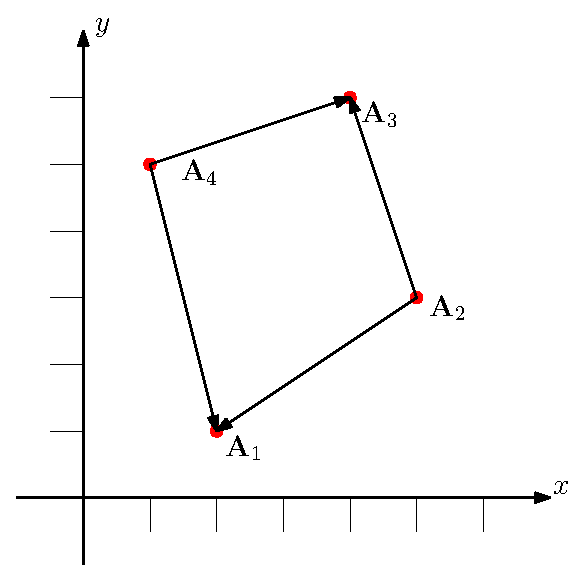
\includegraphics[width=7cm]{img/01/vectores_cuerpo}
 \caption[Cálculo del área de un cuadrilátero]{ 
Aquí se pueden ver los vectores que representan cada uno de los lados, y que son calculados por la resta de los vectores de posición de los puntos.
 } \label{vectorArista:fig}
\end{figure}

Para calcular el área del triángulo $\bigtriangleup \textbf{A}_1 \textbf{A}_3 \textbf{A}_4$ tomamos a $\textbf{A}_4$ como origen y calculamos el vector que va de $\textbf{A}_4$ a $\textbf{A}_1$, luego calculamos el vector que va de $\textbf{A}_4$ a $\textbf{A}_3$, y por último calculamos el producto cruz, tomamos su norma y lo dividimos entre dos.\footnote{Este es un teorema muy conocido de la geometría vectorial y se puede ver en cualquier libro que incluya una introducción a los vectores, me imagino que no necesito citar alguna fuente en especial}
De manera análoga para el siguiente triángulo:

El cálculo de los vectores es el siguiente:
\begin{eqnarray}
\overrightarrow{A_4 A_1} & = \textbf{A}_1 - \textbf{A}_4 = & (1, -3) \nonumber \\
\overrightarrow{A_4 A_3} & = \textbf{A}_3 - \textbf{A}_4 = & (3, 1) \nonumber \\
\overrightarrow{A_2 A_1} & = \textbf{A}_1 - \textbf{A}_2 = & (-3, -2) \nonumber \\
\overrightarrow{A_2 A_3} & = \textbf{A}_3 - \textbf{A}_2 = & (-1, 2) \nonumber
\end{eqnarray}

Y por lo explicado anteriormente el área total de la tapa $A_T$ es:

$$ A_T = A_{\bigtriangleup \textbf{A}_1 \textbf{A}_3 \textbf{A}_4} + A_{\bigtriangleup \textbf{A}_1 \textbf{A}_2 \textbf{A}_3} $$
$$ A = \frac{1}{2} | \overrightarrow{\textbf{A}_4 \textbf{A}_1} \times \overrightarrow{\textbf{A}_4 \textbf{A}_3} | + \frac{1}{2} | \overrightarrow{\textbf{A}_2 \textbf{A}_1} \times \overrightarrow{\textbf{A}_2 \textbf{A}_3} |$$
$$A = \frac{1}{2} | 10 | + \frac{1}{2} | -8 |$$
$$A = 9$$

Ahora sólo nos falta calcular la fuerza $\textbf{F}_p$ y acumularla en cada una de las caras laterales de la caja. Para esto y sólo por simplicidad supongamos que escogemos $k_d = 10$ entonces el cálculo de la fuerza debe hacerse por separado para cada una de las caras laterales (que en nuestro caso equivalen a los lados de la tapa):

\begin{eqnarray}
F_{\overline{\textbf{A}_1 \textbf{A}_2}} & =  \frac{1}{V}\overline{\textbf{A}_1 \textbf{A}_2} k_g & = \frac{1}{9} \sqrt{13} \left( 10 \right) \nonumber \\
F_{\overline{\textbf{A}_2 \textbf{A}_3}} & =  \frac{1}{V}\overline{\textbf{A}_2 \textbf{A}_3} k_g & = \frac{1}{9} \sqrt{5}  \left( 10 \right) \nonumber \\
F_{\overline{\textbf{A}_3 \textbf{A}_4}} & =  \frac{1}{V}\overline{\textbf{A}_3 \textbf{A}_4} k_g & = \frac{1}{9} \sqrt{10} \left( 10 \right) \nonumber \\
F_{\overline{\textbf{A}_4 \textbf{A}_1}} & =  \frac{1}{V}\overline{\textbf{A}_4 \textbf{A}_1} k_g & = \frac{1}{9} \sqrt{10} \left( 10 \right) \nonumber
\end{eqnarray}

Con lo que tenemos la magnitud de las fuerzas que actúan en cada cara, así que sólo falta calcular un vector unitario normal a la cara correspondiente para poder acumular su fuerza.

Afortunadamente, para calcular un vector normal en dos dimensiones, tenemos un método sencillo, el producto punto de dos vectores normales entre sí debe de dar cero, así que si queremos un vector normal al vector $\textbf{v}=(x, y)$ simplemente construimos uno tal que su producto punto con el primero siempre sea igual a cero, por ejemplo $\textbf{v}^n = (-y, x)$.
Con esto sabemos que el vector $\textbf{v}^n$ es siempre normal al vector $\textbf{v}$, de hecho en dos dimensiones sólo este vector y sus múltiplos son normales a $\textbf{v}$.

Sabiendo todo lo anterior, ya se puede acumular la fuerza correspondiente sobre cada cara. Por ejemplo, sobre la primera cara que está definida por el segmento que une a $\textbf{A}_1$ y $\textbf{A}_2$.
Como en el paso anterior ya se había calculado el vector $\overrightarrow{\textbf{A}_2 \textbf{A}_1} = (-3,-2)$ que en sí representa a la cara, podemos calcular su vector normal con la fórmula anterior.
Para esta cara el vector $\textbf{n}=(2,-3)$ es el vector normal, para hacerlo unitario lo dividimos entre su norma $\frac{\textbf{n}}{|\textbf{n}|} = \frac{1}{\sqrt{13}} (2, -3)$.
Y finalmente el vector fuerza que estamos buscando para esta cara en particular es:

$$\textbf{F}_{\overline{\textbf{A}_1 \textbf{A}_2}} = \frac{1}{V}\overline{\textbf{A}_1 \textbf{A}_2} k_g \vec{n} = \frac{1}{9} \sqrt{13} \left( 10 \right)  \frac{1}{\sqrt{13}} (2, -3) = \frac{10}{9}(2, -3) $$

Una consideración más que debe tenerse, al calcular el vector normal, pudiera darse el caso que éste dirija la fuerza al contrario de como se desea, es decir que la dirija, al centro del cuerpo en vez de hacia afuera.
Como se ilustra en la Figura \ref{presionMal:fig}.
En cuyo caso hay que multiplicar este vector normal por $-1$.
En general la mejor práctica es graficar el cuerpo para así poder calcular el vector normal correcto.

Por ejemplo, al calcular un vector normal para la segunda cara podríamos vernos tentados a repetir el cálculo, ocupando el vector que acabamos de calcular $\overrightarrow{\textbf{A}_4 \textbf{A}_1}$ pero al ocupar la fórmula, nos daría $n=(3,1)$ que en efecto es un vector normal a $\overrightarrow{\textbf{A}_4 \textbf{A}_1}$ pero que apunta hacia el centro del cuerpo, y por lo tanto sería incorrecto ocuparlo para dirigir la fuerza de presión.
El vector correcto para este caso es $-n = (-3,-1)$.
Así que se debe tener cuidado al calcular el vector para dirigir la fuerza de presión.

\begin{figure}
 \centering
 \includegraphics[width=7cm]{img/01/presion_mal}
 \caption[Vectores de presión incorrectos]{ 
 Aquí se pueden ver los vectores incorrectos para dirigir la presión pues apuntan al centro de la figura.
 } \label{presionMal:fig}
\end{figure}

El resto de las operaciones correspondientes al ejemplo se pueden ver en el Cuadro ~\ref{ejemplo:presion}.
En la primera columna de la tabla se muestra la cara a la que se estaba calculando la fuerza, después se muestra el valor escalar de la presión, luego el vector asociado a la cara, que ya habíamos obtenido, después el vector normal resultado del procedimiento antes explicado.
Hay que tomar en cuenta que el vector podría ser que apunte hacia afuera o hacia adentro, y en la tabla ya fue corregido (multiplicándolo por el escalar $-1$).
Y en la última columna aparecen los vectores de fuerza que se estaban buscando, y son los que se requieren para poder acumularse en la ecuación de Newton.

\begin{table}
\ra{1.3}
\begin{center}
\begin{tabular} {@{}lllll@{}}
\toprule
Cara & Fuerza de Presión &  Vector de la cara & Vector Normal & Vector Fuerza \\ \midrule
$\overline{A_1A_2}$ & $\frac{1}{9} \cdot 10 \cdot \sqrt{13} $ & $\overrightarrow{A_2A_1} = (-3,-2)$ & $(\frac{2}{\sqrt{13}}, \frac{-3}{\sqrt{13}})$ & $(\frac{20}{9}, \frac{-30}{9})$ \\
$\overline{A_2A_3}$ & $\frac{1}{9} \cdot 10 \cdot \sqrt{5} $ & $\overrightarrow{A_2A_3} = (-1,2)$ & $(\frac{2}{\sqrt{5}}, \frac{1}{\sqrt{5}})$ & $(\frac{20}{9}, \frac{10}{9})$ \\
$\overline{A_3A_4}$ & $\frac{1}{9} \cdot 10 \cdot \sqrt{10} $ & $\overrightarrow{A_4A_3} = (3,1)$ & $(\frac{-1}{\sqrt{10}}, \frac{3}{\sqrt{10}})$ & $(\frac{-10}{9}, \frac{30}{9})$ \\
$\overline{A_1A_4}$ & $\frac{1}{9} \cdot 10 \cdot \sqrt{10} $ & $\overrightarrow{A_4A_1} = (1,-3)$ & $(\frac{-3}{\sqrt{10}}, \frac{-1}{\sqrt{10}})$ & $(\frac{-30}{7}, \frac{-10}{9})$ \\ 
\bottomrule
\end{tabular}
\end{center}
\caption[Ejemplo sobre cómo calcular la fuerza de presión]{Cálculo de la Fuerza de Presión, para el ejemplo}
\label{ejemplo:presion}
\end{table}

La fuerza de presión es mucho más compleja de calcular que las fuerzas debidas a la gravedad y a los \emph{resortes-amortiguadores}.
La principal dificultad es que debe tratar con la geometría del cuerpo para calcularla, además es necesario conocer el volumen total del cuerpo, y por cada cara que se acumule se debe de conocer: el área de la misma y un vector normal, por lo que a diferencia de los casos anteriores no hay una manera general de enunciar las fórmulas sino que debe analizarse el caso particular de la geometría del cuerpo que se esté tratando.

\begin{figure}
 \centering
 \includegraphics[width=7cm]{img/01/presion_bien}
 \caption[Vectores de presión correctos]{ 
 Así es como debe de dirigirse la fuerza de presión. Obsérvese que cada esquina debe acomular la fuerza de las dos caras laterales que está uniendo.
 } \label{presionBien:fig}
\end{figure}

 
\chapter{Construcción del algoritmo de simulación}

En este capítulo nos encargaremos de presentar el algoritmo propuesto por Matyka en~\cite{Matyka:Presion}, que es explicado en más detalle en~\cite{Matika:SoftBody}.
Este modelo no es más que la unión de los modelos del capítulo anterior.
Además definiremos el experimento que deseamos realizar para probar el funcionamiento del modelo.

Más adelante en este mismo capítulo, explicaremos cómo se pueden enfrentar ciertos detalles sobre el algoritmo de Matika.

Primero veremos cómo se puede calcular el volumen de un cuerpo en tres dimensiones, explicaremos cómo se puede tener una idea general, y por qué para ciertas geometrías del cuerpo, se prestan mejor ciertos algoritmos.

Luego nos enfrentaremos al problema de cómo integrar la ecuación de Newton, con métodos numéricos, analizando dos alternativas, y se presentan las que se consideran las mejores maneras de implementar el integrador en código.

Por último analizaremos el problema más difícil de la implementación: las colisiones.
Esto se analiza en dos partes, la manera como se detectan y la respuesta de las mismas.

\section{Diseño del experimento}
\label{descripcion:experimento}
Necesitamos una simulación gráfica (animación) y el principal objetivo será hacer que se \emph{vea} real.

Se quiere modelar un cuerpo neumático.
Para hacerlo partimos de un cuerpo flexible y le ponemos un fluido dentro, en este caso el gas, además queremos una manera de probar cómo es la interacción de éste con otros objetos de la escena. 

Con base en esos requerimientos, diseñe la siguiente situación: se modela una caja cerrada, en la cual su cara superior tiene la característica de ser formada como un cuerpo flexible, las otras cinco caras son rígidas.
Dentro de esta caja se pone el fluido (gas), de manera que ahora tenemos un cuerpo neumático.
Para probar su interacción con otro cuerpo se le deja caer sobre su cara flexible un cuerpo sólido (en este caso una esfera) y se observa el resultado.

Además para poder hacer varios tipos de pruebas se desea que la animación tenga cierta interactividad, es decir que el usuario pueda, en tiempo de ejecución, cambiar algunas opciones tanto de visualización como también algunos parámetros físicos.

Esta simulación es el objetivo principal del trabajo, y el siguiente capítulo está dedicado a cómo se construyó, mientras que en este capítulo se hace énfasis en los detalles teóricos necesarios para escribir el programa.

\section{Simulaciones gráficas basadas en física}

Lo primero que debemos de hacer es exponer las condiciones de nuestra simulación de cuerpo flexible. La situación física que deseamos modelar es la de un cuerpo flexible, hueco que contiene un gas.
Por ejemplo, imagínese un globo, un colchón de aire, la llanta de un automóvil o una burbuja.
El comportamiento en el que estamos interesados es en un comportamiento cualitativamente parecido al del fenómeno, es decir que al momento de graficarlo y hacer una animación debe verse \emph{parecido} al sistema real.

El valor de poder graficar de manera realista un modelo como éste, radica en el hecho de que hay muchas cosas que se comportan de manera parecida, y al momento de animar una escena donde hay varios de estos objetos, un modelo físicamente más realista sería muy costoso en tiempo de ejecución.

La forma de atacar este problema será hacerlo con un modelo simple.
Imagínese un cuerpo formado por varios puntos unidos entre ellos por resortes.~\footnote{Este modelo es muy socorrido cuando se trata de modelar ropa o tela, se pueden ver ejemplos en el último capítulo de~\cite{FisicaVideojuegos}, que modela una bandera o en~\cite{Vassilev:Ropa} y~\cite{Provot:Ropa}, ambos modelan ropa sobre una persona}
Ahora imagínese que a un cuerpo cerrado formado por esta \emph{tela}, le ponemos dentro una fuente de aire, que le ayuda a mantener su forma más o menos constante durante las deformaciones permitidas por los resortes que lo forman; ésa es la idea principal de nuestro modelo.

En la Figura~\ref{modelo:fig} podemos ver un pequeño esquema del modelo, en este caso es un hexágono en dos dimensiones.
Desde luego, mientras más compleja sea la forma de nuestro modelo, mas difícil será trabajar con él, pero se verá más realista 

\begin{figure}
 \centering
 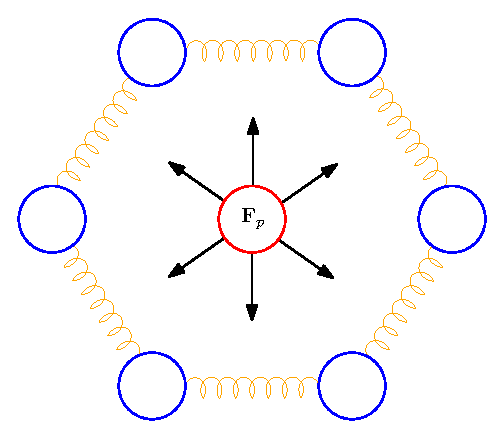
\includegraphics[]{img/02/modelo}
 \caption[Diagrama del modelo masa, resorte, y presión]{ 
 Un ejemplo de un modelo de masa resorte, con presión. Se trata de un hexágono cerrado, y $\textbf{F}_p$ representa la fuerza debida a la presión.
 } \label{modelo:fig}
\end{figure}

\subsection{Esbozo general del algoritmo}
Una vez conocida la idea, nos empezaremos a preguntar en cómo llevarlo a cabo, es decir cómo podemos implementar este modelo en forma de un algoritmo que seamos capaces de codificar en algún lenguaje de programación.


\begin{figure}
 \centering
 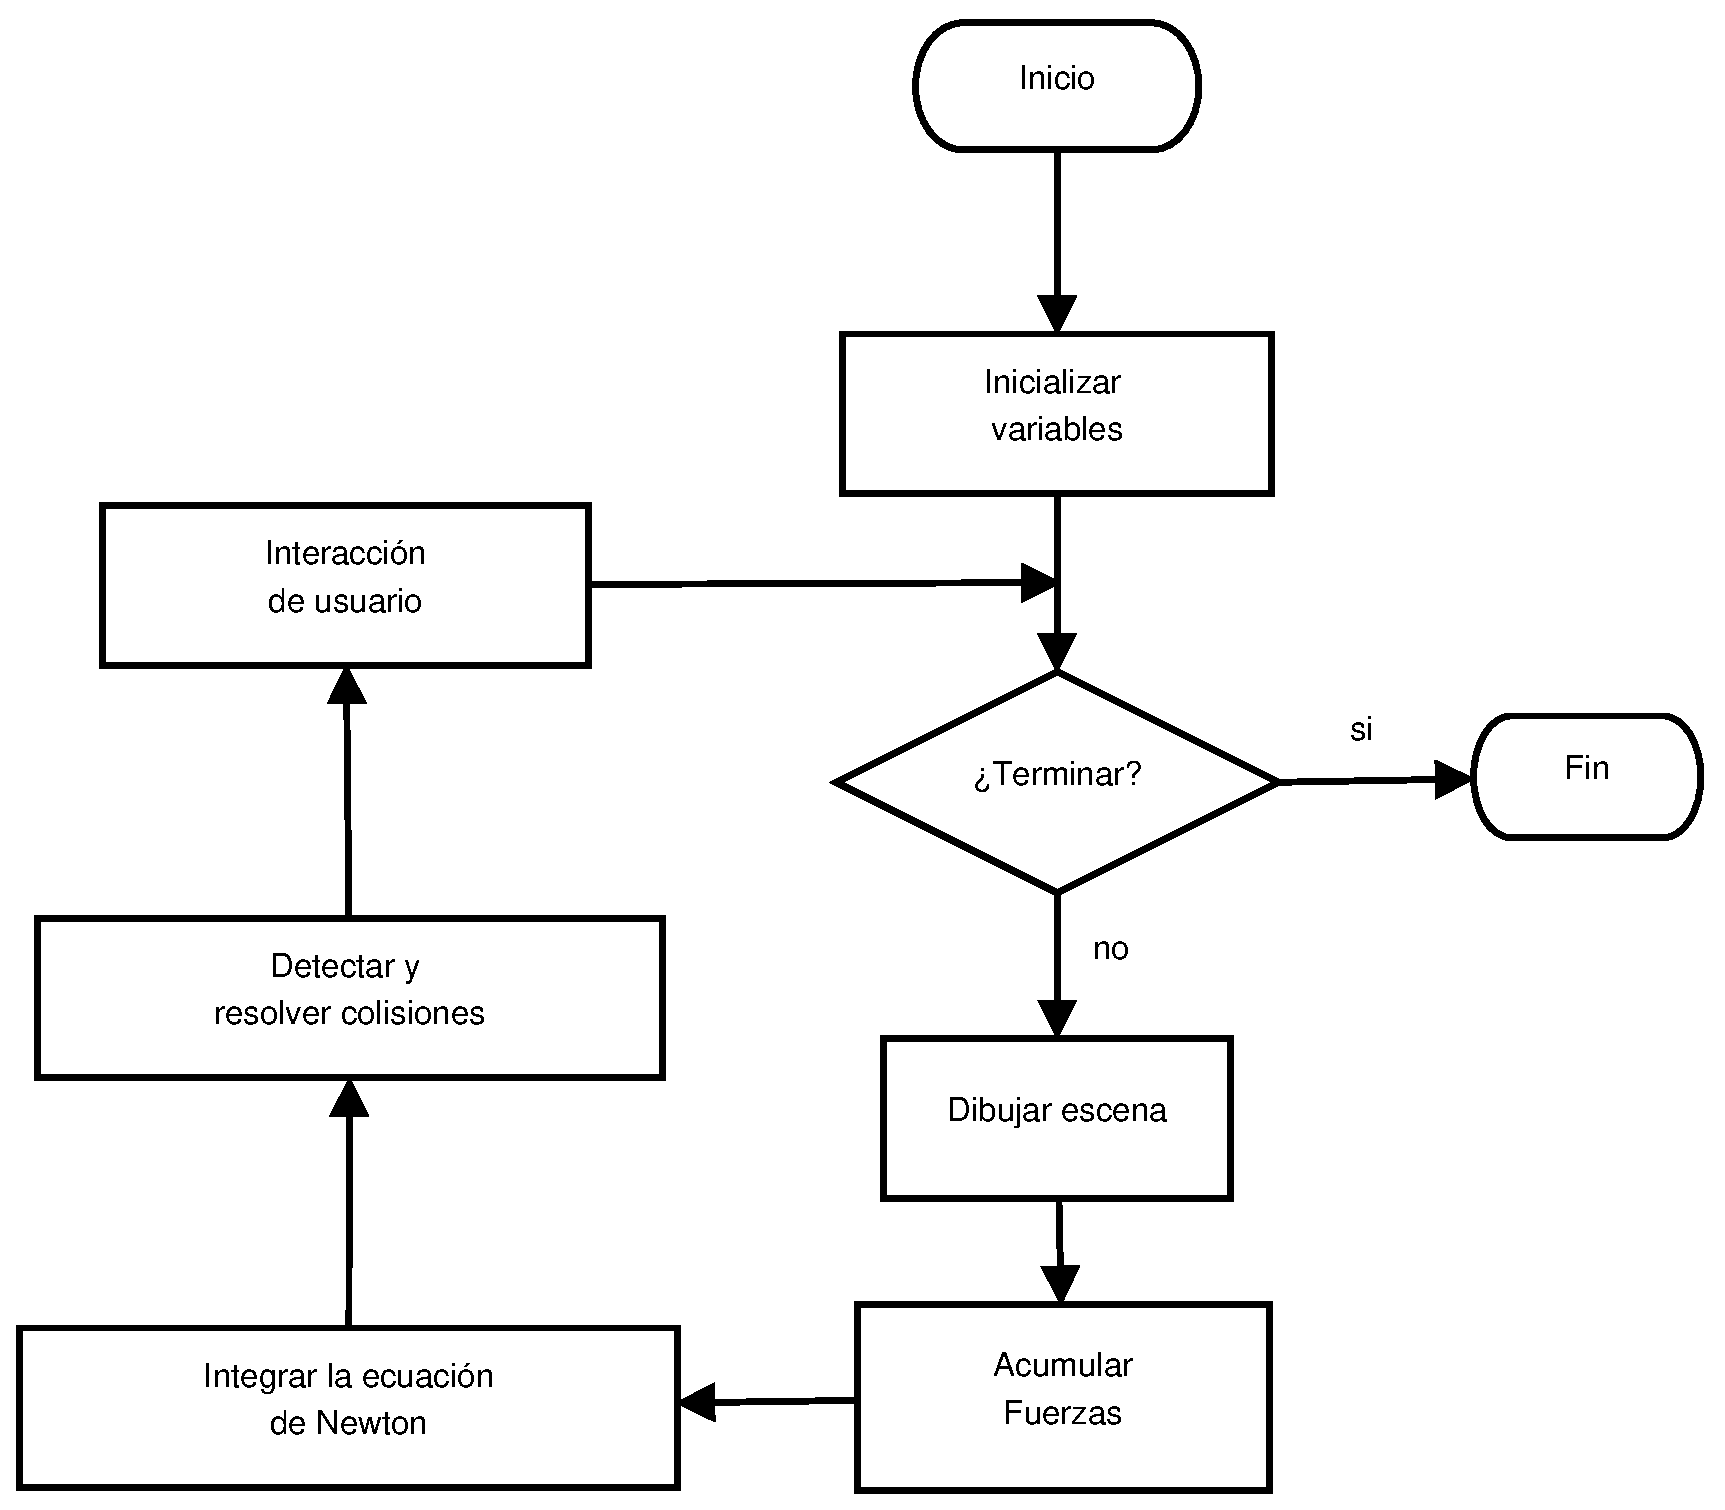
\includegraphics[width=10cm]{img/02/diagrama_flujo}
 \caption[Diagrama de flujo de la simulación]{ 
 Este diagrama de flujo muestra, los detalles generales a seguir en una simulación gráfica basada en física. Para cada paso del algoritmo se pueden tener diferentes estrategias, pero en general este esquema no debe cambiar.
 } \label{diagrama_flujo:fig}
\end{figure}

El diagrama de flujo del algoritmo es el que se muestra en al Figura~\ref{diagrama_flujo:fig}, en donde se puede apreciar que sólo se tienen bloques de proceso; cada uno de estos procesos puede ser llevado a cabo de muchas maneras, pero tendrá que ser en este orden, en esta sección veremos con un poco más de detalle cada proceso.

\subsubsection{Inicializar variables}
Lo primero es dar valor a las variables que lo necesiten, me refiero con esto a variables globales, que afectan cómo funciona el programa por el resto de su ejecución.
Dentro de estas variables están los parámetros externos del modelo, es decir esos que no pueden ser calculados dentro del programa y que es necesario que se proporcionen por el usuario.
Los parámetros necesarios son $m$ para cada partícula, $g$, $k_d$ y $k_s$ para los resortes, $L$ para cada resorte en particular, y $k_g$ para la acumulación de la fuerza debida a la presión.

Otra cosa que debe hacerse en este paso del algoritmo es poner las condiciones iniciales del modelo, por ejemplo, la posición de cada partícula y la velocidad al momento de iniciar la animación.
Y de igual manera con los cuerpos no flexibles que deseemos que interactúen con nuestro modelo, se debe de conocer su posición, si se mueven o no, y cómo van a interactuar con el modelo.

Por último las opciones globales, que afecten a la animación también se deben de obtener aquí, por ejemplo el tamaño del paso $\Delta t$ para mover el modelo, las opciones de los gráficos (si se hará \emph{\textenglish{render}}, o se tratará sólo con el \emph{\textenglish{wireframe}}~\footnote{Cuando sólo se dibujan los bordes de las figuras, como si éstas estuvieran hechas de una malla de alambre se le llama wireframe, cuando dibujamos el área de las figuras y les damos color y efectos de iluminación se dice que se les dio \emph{render}.}) y qué tipo de integrador se ocupará en el modelo.
Alguien me podría decir que estos también son parámetros.
Y en efecto lo son, quise sin embargo hacer la distinción y llamarlos variables globales, por el hecho de que no se deben al modelo en sí, sino más bien a la implementación que cada quien haga del mismo, es decir se deben al programa.

\subsubsection{Dibujar escena}
Esta parte del algoritmo debe ser la encargada de dibujar en la pantalla toda la escena.
Para hacer esto debe contar con la información de donde se encuentran cada punto y donde se encuentra cada cosa que queramos dibujar.

Aunque no hay mucho que decir aquí, ésta parte es delicada, depende de nuestro conocimiento de las herramientas que vamos a usar para hacer el programa.
Con la ayuda de una biblioteca gráfica, en este caso \emph{\textenglish{OpenGL}}, y los datos necesarios guardados de una manera ordenada, como en una estructura de datos, debemos de ser capaces de implementar esta función.

El detalle de la implementación depende del modelo en cuestión, veré a detalle la que yo use.
Esto puede ser útil para que alguien que deseé implementar una simulación, se de algunas ideas, pero como ya dije, esta parte depende del fenómeno a modelar, por lo que en cada implementación se debe de hacer un análisis.

\subsubsection{Acumular fuerzas}
Las fuerzas que actúan sobre cada partícula del modelo, se pueden identificar como \emph{externas}, es decir que se deben al medio, o \emph{internas} que se deben al cuerpo en sí.
Ejemplos de fuerzas externas son la gravedad, la viscosidad del medio, la resistencia del aire, por mencionar algunas.
Ejemplos de las fuerzas internas son por otra parte: los \emph{resortes amortiguadores} y la debida a la presión del gas.

Cualquiera que sea el caso, en este paso debemos de calcular todas las fuerzas que intervienen en nuestro modelo, y debemos de acumulársela a cada uno de las partículas que lo conforman, es decir, cada partícula debe tener asociada la suma de todas las fuerzas que actúan sobre ella.
Recordemos que la fuerza en general es un vector, por lo que la acumulación de la que hablo es una suma vectorial de cada una de las fuerzas.

Los detalles de cómo acomular las fuerzas específicas que ocuparé en la simulación se darán en la siguiente sección y con más a detalle en el resto del capítulo.

\subsubsection{Integrar la ecuación de Newton}
Las fuerzas acomuladas en el paso anterior, junto con la posición y velocidad actuales de la partícula, nos proporcionan (como dice la segunda ley de Newton~\eqref{ley:Newton}) el siguiente estado, nos dan la información suficiente para saber la nueva posición y la nueva velocidad de la partícula en cuestión. 
Conociendo esto para todas las partículas tendremos determinado el estado completo del modelo en el tiempo siguiente.

Como ésta es una ecuación diferencial, debemos de resolverla, o mejor dicho integrarla, para conocer el siguiente estado del sistema, sin embargo como nuestra acumulación de fuerzas fue hecha a partir de muchas fuerzas, todas ellas de naturaleza distinta, no podremos integrar esta ecuación de manera analítica.
Por esta razón debemos de recurrir a un método numérico que nos permita aproximar la solución.

Por suerte hay muchísimos métodos numéricos que se ajustan a nuestras necesidades, aquí he decidido presentar a dos de ellos solamente, en la sección dedicada a integrar la ecuación de Newton explicaré a detalle cómo funcionan.
De manera general, se puede decir que todos ellos toman como información la posición y velocidad actual de la partícula, el vector fuerza que actúa sobre ella y el instante de tiempo que pasa entre el estado actual y el nuevo estado que queremos calcular (ésta cantidad es $\Delta t$).
Y después de hacer cálculos con ellos nos devuelven un nuevo estado, en forma de la nueva posición y la nueva velocidad de la partícula.

\subsubsection{Detectar y resolver colisiones}
En este paso debemos analizar qué pasa cuando nuestro modelo choca o interactúa con otros objetos de la escena.
Estos otros objetos pueden ser cuerpos rígidos como el piso o flexibles como otro cuerpo de la misma característica del nuestro.

El segundo paso es la respuesta a esta colisión.
Este problema es también delicado, pero en general, se va a encargar de ver la partícula que chocó, moverla como respuesta al choque y modificar su estado, es decir su posición y su velocidad.
En una sección posterior de este capítulo hablaré con más detalle y también daré algunas ideas generales.

\subsubsection{Interacción del usuario}
Este paso es opcional, y depende de si deseamos que la simulación tenga una forma de ejecutarse independiente del usuario o si se desea que éste pueda cambiar la simulación en tiempo de ejecución, por ejemplo modificando algún parámetro de la simulación.

Para enfrentar esto se tiene que recurrir totalmente a la creatividad del programador que vaya a hacer la implementación.
Una buena idea es por ejemplo utilizar alguna biblioteca que exista precisamente para este fin. En éste caso se decidió utilizar un par de bibliotecas que se integran bien con \emph{\textenglish{OpenGL}}.
Por un lado \emph{\textenglish{glfw}}, que permite manejar eventos del ratón y del teclado. 
Y por otro lado \emph{\textenglish{Dear Imgui}} que permite implementar una interfaz gráfica (menú) de usuario.

\section{El sistema de fuerzas}
Es momento de hacernos unas preguntas:
¿Qué es lo que compone nuestro cuerpo?
¿Qué necesitamos saber para implementar este modelo?
La primera pregunta es sencilla: nuestro cuerpo está formado por puntos, que están unidos por resortes, que a su vez se unen para formar las caras.
Resumiendo, nuestro cuerpo es un conjunto de caras, que a su vez son un conjunto de resortes, que a su vez son un conjunto de puntos:
¡Nuestro cuerpo está formado por puntos (partículas)!
La respuesta de la segunda interrogante está ligada a la primera, necesitamos saber todo lo que sea necesario para poder acumular fuerza a las partículas, es decir que para cada una debemos de poder ocupar las ecuaciones~\eqref{fuerzaGravedad}, ~\eqref{fuerzaResorte} y \eqref{fuerzaGas}.

Ciertamente cada una de estas fuerzas es de naturaleza distinta, la fuerza de gravedad es externa y se puede calcular para cada partícula por separado, la de los resortes depende de la posición de cada partícula y de sus vecinos a los cuales está conectado por un \emph{resorte-amortiguador} y por último la de la presión depende de la cara en la que esté la partícula y del volumen total del cuerpo.
Podemos resumirlo en el Cuadro~\ref{ejemplo:fuerzas}.

\begin{table}
\ra{1.2}
\begin{center}
\begin{tabular} {@{}llll@{}} 
\toprule
Fuerza & Símbolo &  Parámetros & Datos necesarios \\ 
\midrule
Gravedad & $ \textbf{F}_g $ & $g$, $m$ & Ninguno \\
Resorte & $ \textbf{F}_s + \textbf{F}_d $ & $k_s$, $k_d$ & Partículas unidas por el resorte \\
& & & Velocidad y posición de cada partícula que une el resorte \\
Presión & $ \textbf{F}_p $ & $k_g$ & Partículas que forman la cara \\ 
& & & Volumen total del cuerpo \\ 
& & & Area de la cara \\ 
\bottomrule
\end{tabular}
\end{center}
\caption[Resumen de las fuerzas que actúan sobre cada partícula]{Fuerzas a calcular para cada partícula y que se necesita saber para hacer los cálculos}
\label{ejemplo:fuerzas}
\end{table}

Para calcular la fuerza de gravedad es necesario que se conozcan dos parámetros, la masa de cada partícula $m$, y la constante gravitación $g$.
La gravedad debe de acumularse en cada partícula.

La fuerza del \emph{resorte amortiguador} es una fuerza interna.
Para calcularla  necesitamos recibir dos parámetros: $k_s$ y $k_d$.
Luego necesitamos calcular la posición y la velocidad de cada partícula, y saber por cada resorte qué partículas está uniendo.
Cuando tengamos que acumular esta fuerza recorreremos todos los resortes y por cada resorte calcularemos una fuerza, luego la acomularemos en cada unos de las dos partículas a los que este resorte esté conectado.

Por último, para la fuerza debida a la presión, necesitamos un parámetro externo: $k_g$.
Y para poder calcular esta fuerza debemos conocer antes de empezar el volumen total del cuerpo $V$, luego debemos de saber qué partículas pertenecen a cada una de las caras del cuerpo.
Para acumular esta fuerza debemos recorrer cada una de las caras que forman el cuerpo, en cada caso calculamos el área de la cara y acumulamos la fuerza $\textbf{F}_p$ que le corresponda en cada una de las partículas que la forman.

\section{Área, volumen y vectores normales}
Los parámetros necesarios para calcular la fuerza de presión son el volumen total del cuerpo, el área de cada una de las caras, y un vector normal a dicha cara; como ya se dijo, esto depende enteramente de la geometría del cuerpo que se quiera modelar.
Sin embargo, esto no quiere decir que no se puedan dar algunas técnicas generales que en alguna medida puedan ser adaptadas a alguna geometría particular.
El propósito de esta sección es precisamente el de explicar esas técnicas generales.

\subsection{Cálculo de áreas}
Para calcular el área de un cuerpo geométrico generalmente se calcula el área de cada una de sus caras y después se suman.
Empezando por el caso más simple, supongamos que tenemos un triángulo formado por tres puntos, sabemos las coordenadas de cada uno de los puntos, y queremos su área.
Supongamos que los puntos son denotados por $\textbf{P}$, $\textbf{Q}$ y $\textbf{R}$.
Podemos calcular dos de las aristas del triángulo si calculamos los vectores que van de $\textbf{P}$ a $\textbf{Q}$ y de $\textbf{P}$ a $\textbf{R}$.
Luego podríamos calcular el producto cruz de los dos vectores que acabamos de encontrar y obtener su norma, finalmente la mitad de la norma sería el área del triángulo que estamos buscando.

$$\overrightarrow{\textbf{PQ}} = \textbf{Q} - \textbf{P}$$
$$\overrightarrow{\textbf{PR}} = \textbf{R} - \textbf{P}$$
$$ A = \frac{1}{2} \vert \overrightarrow{\textbf{PQ}} \times \overrightarrow{\textbf{PR}} \vert$$

Si queremos calcular el área de un cuadrilátero podemos usar la idea anterior y \emph{triangular}, el cuadrilátero en dos partes, supongamos que queremos calcular el área del cuadrilátero formado por los puntos $\textbf{P}$, $\textbf{Q}$, $\textbf{R}$ y $\textbf{S}$, podríamos calcular el área del triángulo $\triangle \textbf{PQR}$ y luego sumar el área del triángulo $\triangle \textbf{SRQ}$.
Dicho de otra manera:

\begin{eqnarray} 
A_{T} & = & A_{\triangle \textbf{PQR}} + A_{\triangle \textbf{SRQ}} \nonumber \\
A_{T} & = & \frac{1}{2} \vert \overrightarrow{\textbf{PQ}} \times \overrightarrow{\textbf{PR}} \vert \times \frac{1}{2} \vert \overrightarrow{\textbf{SQ}} \times \overrightarrow{\textbf{SR}} \vert \nonumber \\
\label{formulaArea}
A_{T} & = & \frac{1}{2} \left( \vert \overrightarrow{\textbf{PQ}} \times \overrightarrow{\textbf{PR}} \vert + \vert \overrightarrow{\textbf{SQ}} \times \overrightarrow{\textbf{SR}} \vert \right)
\end{eqnarray}

Este resultado de hecho, puede ampliarse aún más con el enunciado siguiente:

Sea $P$ un polígono simple, sin agujeros, dado por la secuencia ordenada de vértices $\textbf{P}_i = (x_i, y_i)$, $i = 1,\ldots,n$, (por ejemplo en el sentido contrario a las agujas del reloj), entonces el área de $P$ es:
$$A(P) = \frac{1}{2}\sum^{n-1}_{i = 1} \det (\textbf{P}_i, \textbf{P}_{i + 1}) + \frac{1}{2} \det (\textbf{P}_n, \textbf{P}_1)$$

Este teorema fue tomado de \cite{GeometriaParaCAD} donde también es demostrado. 
Con la adecuada combinación de estas técnicas es sencillo ingeniárselas para poder calcular el área de una cara.

\subsection{Cálculo de volúmenes}
Calcular volúmenes es usualmente más complejo que calcular áreas, y por ende casi siempre es computacionalmente costoso, de ahí que además de maneras geométricas de calcular un volumen siempre está la alternativa de aproximar un volumen.
De nuevo hay que pensar qué queremos lograr con la simulación si rapidez en la ejecución, o apego a la realidad física.

No hay que olvidar también que para todo modelo y sus respectivos parámetros, siempre hay diferentes grados de sensibilidad, por ejemplo en el caso de nuestro modelo el volumen sólo es utilizado para poder determinar la fuerza escalar de la presión, por lo que es un modelo \emph{poco sensible} al cálculo del volumen.
Es decir, es válido aproximarse en este rubro en este rubro, sin perder mucha realidad en el modelo.

\subsubsection{Volúmenes aproximados}
Hay varias formas de aproximar el volumen de un cuerpo, una de ellas es con cajas envolventes o \emph{\textenglish{bounding boxes}}, la idea es muy simple se trata de aproximar el volumen de un cuerpo complejo mediante el volumen de un cuerpo simple que lo contenga.
Es decir, se aproxima el volumen por medio de poliedros regulares ya sean inscritos o circunscritos, tales que den una buena aproximación del cuerpo cuyo volúmen estamos calculando.

Una forma más simple es aproximando con un \emph{hexaedro regular} cuyo volumen es $ l \cdot w \cdot h $, o largo por alto por ancho; otra forma geométrica que se usa de manera muy común es el \emph{elipsoide}, cuyo volumen es $ \frac{4\pi}{3} a \cdot   b \cdot  c $, donde $a$, $b$ y $c$, son los largos de sus ejes principales.

\subsubsection{Volúmenes Exactos}
Una técnica muy útil para calcular el volúmen de una malla triangular se puede ver en~\cite{Zhang:volumen}.

La técnica consiste recorrer todas la caras, y en cada una calcular el \emph{volumen orientado} del tetraedro cuya base es la cara triangular y cuya punta es el origen del sistema de referencia.
El signo del volumen (por eso dijimos que es un volumen orientado) depende de si el tetraedro apunta hacia el origen.
Eso quiere decir que habrá algunos volúmenes que sean negativos y otros positivos, la suma de todos los volúmenes es el volumen de la malla.

Es importante que al usar esta fórmula, los triángulos apunten hacia el mismo lado de la malla.
En otras palabras, se deben de definir un orden para los vértices de los triángulos (por ejemplo en contra de las manecillas del reloj) y se debe ser consistente en toda la malla.
En efecto, esta técnica usa una normal a la cara del triángulo para orientar, pero dicha normal está implícita por el orden de los vértices.

En resumen el volumen del la malla formada por $n$ caras triangulares está dado por:

\begin{equation}
V = \frac{1}{6} \sum_{i=1}^{n} \textbf{g}_i \cdot \textbf{N}_i
\label{eq:volumen}
\end{equation}

En donde $\textbf{g}_i$ y $\textbf{N}_i$ son el baricentro y la normal del triángulo $i$. Y asumiendo que dicho triángulo tiene vértices en el orden $\textbf{v}_{i}^{1}$, $\textbf{v}_{i}^{2}$ y $\textbf{v}_{i}^{3}$ se pueden calcular de la siguiente manera:

\begin{equation}
\textbf{g}_{i} = \frac{(\textbf{v}_{i}^{1} + \textbf{v}_{i}^{2} + \textbf{v}_{i}^{3})}{3}
\label{eq:baricentro}
\end{equation}

\begin{equation}
\textbf{N}_i = (\textbf{v}_{i}^{2} - \textbf{v}_{i}^{1}) \times (\textbf{v}_{i}^{3} - \textbf{v}_{i}^{1})
\label{eq:normTriag}
\end{equation}

Como ya se dijo, se puede transformar cualquier malla poligonal en una malla triangular subdividiendo cada cara en triángulos.
Por ejemplo, nuestro cuerpo neumático está formado por caras en forma de cuadriláteros.
Cada cara se puede partir por su diagonal para formar dos triángulos.

\subsection{Vectores normales}
Dado un plano podemos encontrar un vector que le sea normal, sólo necesitamos dos vectores linealmente independientes que se encuentren en el plano y calculando su producto cruz obtenemos un vector normal, es decir en términos más simples, si conocemos tres puntos del plano y no son colineales, podemos calcular el vector perpendicular a ese plano.

Matemáticamente: dado el triángulo formado por los puntos $\textbf{A}_1 = (x_1, y_1, z_1)$, $\textbf{A}_2 = (x_2, y_2, z_2)$ y $\textbf{A}_3 = (x_3, y_3, z_3)$, un vector normal a este plano, es el vector $\textbf{n}$ que se calcula:

$$ \textbf{n} = \overrightarrow{\textbf{A}_1 \textbf{A}_2} \times \overrightarrow{\textbf{A}_1 \textbf{A}_3}$$

Un hecho muy importante es que si queremos calcular el vector normal a una superficie, podemos calcular los vectores normales a cada vértice de ella y luego promediarlos.
Esto por increíble que parezca funciona y es de hecho la manera como se hacen los cálculos de iluminación en la mayoría de los programas de CAD y de simulación gráfica.

Es decir, si tenemos el polígono de $n$ lados, formado por los puntos $\textbf{P}_1, \textbf{P}_2, \ldots, \textbf{P}_n$, ordenados de alguna manera, por ejemplo en sentido contrario a las manecillas del reloj, y queremos el vector normal a este polígono $\textbf{n}$, calculamos los vectores $ \textbf{v}_1, \textbf{v}_2, \ldots , \textbf{v}_n $, de la forma $\textbf{v}_i = \overrightarrow{\textbf{P}_i \textbf{P}_{i + 1}} \times \overrightarrow{\textbf{P}_i \textbf{P}_{i + 1}} $ para $i = 2, \ldots, n$ y $\textbf{v}_1 = \overrightarrow{\textbf{P}_1 \textbf{P}_2} \times \overrightarrow{\textbf{P}_1 \textbf{P}_n}$, y luego el vector normal $\textbf{n}$ es:

\begin{equation}
\label{formulaVecNormal} 
\textbf{n} = \frac{1}{n} \sum_{i=1}^{n} \textbf{v}_i
\end{equation}

Este hecho es fundamental para nuestros cálculos, tanto de la fuerza debida a la presión, como para la iluminación en el render.
Una demostración se puede encontrar en \cite{GeometriaParaCAD}.

\section{Integrar la ecuación de Newton}
Desde que hay modelos físicos, ha habido interés en la solución numérica de ciertos problemas para los que se sabía de antemano que una solución existía, pero no se contaban con métodos analíticos para encontrarla.
Es por esta razón que nace el análisis numérico, sin embargo no fue hasta que se popularizó el uso de las computadoras que este campo tomó más importancia.

Dentro del análisis numérico, es de nuestro interés la solución numérica de ecuaciones diferenciales.
El problema comienza con una ecuación de primer orden con condición inicial y que cumple las condiciones de existencia y unicidad.

Actualmente, hay muchas maneras de atacar estos problemas, es decir muchas familias de métodos.
Por familia quiero decir que cuando alguien propone un método y llega otra persona más y le hace correcciones, ahora hay dos métodos pero en esencia funcionan con la misma idea, por eso son dos métodos de la misma familia.

El primer método para obtener una aproximación numérica de la solución de una ecuación diferencial es el método de Euler, y desde entonces se han propuesto muchísimos métodos e ideas más.
El Cuadro~\ref{historia:metodos} es una línea del tiempo que tiene algunos de los acontecimientos más importantes del desarrollo de esta disciplina.

\begin{table}
\ra{1.2}
\begin{center}
\begin{tabular} {@{}lp{12cm}@{}} 
\toprule
Año & Evento \\ 
\midrule
1768 & Leonhard Euler publica su método, el primero en la historia \\
1824 & Agustin Cauchy demuestra la convergencia del método de Euler, emplea el método de Euler implícito \\
1855 & En una carta escrita por John F. Bashforth, se mencionan por primera vez los métodos de pasos múltiples de Couch Adams \\
1895 & Carl Runge publica el primer método de Runge Kutta \\ 
1905 & Martin Kutta describe el popular método de Runge Kutta de orden cuatro \\ 
1910 & Lewis Fry Richardson anuncia su método de extrapolación. \\
1952 & Charles F. Curtiss y Joseph Oakland Hirschfelder acuñan el término \emph{\foreignlanguage{english}{stiff equations}}. \\
1967 & Loup Verlet publica su método, especialmente enfocado a la mecánica de partículas \\ 
\bottomrule
\end{tabular}
\end{center}
\caption[Evolución histórica de los métodos numéricos]{Una línea de tiempo que muestra algunos de los acontecimientos más importantes para la solución numérica de ecuaciones diferenciales}
\label{historia:metodos}
\end{table}

En esencia estos métodos se encargan de resolver la ecuación diferencial de la forma:
\begin{eqnarray}
 \frac{d\textbf{y}}{dt} & = &\textbf{F}(t,\textbf{y}) \nonumber \\
 \textbf{y}(t_0) & = & \textbf{y}_0 \label{condicion:inicial}
\end{eqnarray}

Y para hacerlo toman la condición inicial~\eqref{condicion:inicial}, como el primer valor de la solución, con ella calculan un valor aproximado para la solución $\textbf{y}(t)$ en el tiempo $t = t_0 + \Delta t$.
Ahora este nuevo punto de la solución lo llamamos $\textbf{y}_{n}$ y nos ayuda a encontrar un nuevo punto dando otro paso hacia adelante en el tiempo $t = t_0 + 2\Delta t$.
Y así sucesivamente, de manera que la salida de nuestro método son una colección de parejas $(t + n \Delta t, \textbf{y}(t + n \Delta t) )$ la primera de ellas es la condición inicial, y de ahí en adelante se trata de aproximaciones de la solución.

Sin embargo nosotros no queremos resolver una ecuación como ésta, deseamos resolver la ecuación~\eqref{ley:Newton}, que es una ecuación diferencial de segundo orden.
Para poder adaptar este problema al método se propone un cambio de variable $\frac{d\textbf{x}}{dt} = \textbf{v}(t)$, por lo que el problema se transforma en resolver un sistema de dos ecuaciones diferenciales.

\begin{eqnarray}
\frac{d\textbf{v}}{dt} & = & \frac{1}{m} \textbf{F}(\textbf{x}, \textbf{v}, t) \nonumber \\
\frac{d\textbf{x}}{dt} & = & \textbf{v}(t) \nonumber \\
\textbf{v}(0) & = & \textbf{v}_0 \nonumber \\
\textbf{x}(0) & = & \textbf{x}_0 \nonumber
\end{eqnarray}

Los métodos siguientes entonces supondrán que sabemos la velocidad y la posición de la partícula en el tiempo $t$, así como la fuerza que actúa sobre ella en este tiempo, con esta última podremos calcular la posición y la velocidad de la partícula en un tiempo posterior $t + \Delta d$.

\subsection{El método de Euler}
Este método fue el primero de todos, de ahí que también sea el más simple, sin embargo aún tiene algunas ventajas el usarlo.
Básicamente el método de Euler nos dice que si tenemos una ecuación de la forma:
$$\textbf{y}'(t) = \textbf{f}(t, y)$$
Con una condición inicial de la forma $\textbf{y}(0)=\textbf{y}_0$.

Entonces podemos aproximar el siguiente punto de la solución con la siguiente fórmula de recurrencia:

$$\textbf{y}_{n+1} = \textbf{y}_n + h\textbf{f}(t_n, \textbf{y}_n)$$

En donde $h$ representa el tamaño del paso en el tiempo hacia adelante es decir $h = \Delta t$.

El método de Euler se puede generalizar para sistemas de ecuaciones diferenciales de tamaño $n$.
Estas generalizaciones se pueden ver en casi cualquier libro de Ecuaciones y en cualquier libro de análisis numérico.
Aquí sólo daré las fórmulas de recurrencia para el caso de $n=2$ por ser el que estamos interesados en resolver.

Dado el sistema:
\begin{eqnarray}
\textbf{x}'(t) & = & \textbf{f}(t, \textbf{x}, \textbf{y}) \nonumber \\
\textbf{y}'(t) & = & \textbf{g}(t, \textbf{x}, \textbf{y})
\label{sistema:general}
\end{eqnarray}
Con las condiciones iniciales:

\begin{eqnarray}
\textbf{x}(t_0) & = & \textbf{x}_0 \nonumber \\
\textbf{y}(t_0) & = & \textbf{y}_0
\label{condiciones:general}
\end{eqnarray}

Entonces la solución se puede aproximar con las siguientes fórmulas de recurrencia:
$$\textbf{x}_{n+1} = \textbf{x}_n + h\textbf{f}(t_n, \textbf{x}_n, \textbf{y}_n)$$
$$\textbf{y}_{n+1} = \textbf{y}_n + h\textbf{g}(t_n, \textbf{x}_n, \textbf{y}_n)$$

Ahora vamos a poner nuestro sistema de manera que podamos ocupar estas fórmulas para resolverlo:
\begin{eqnarray}
\textbf{v}'(t) & = & \frac{1}{m}\textbf{F}(t, \textbf{x}, \textbf{v}) \nonumber \\
\textbf{x}'(t) & = & \textbf{v}(t, \textbf{x}, \textbf{v})
\label{sistema:particular}
\end{eqnarray}

Y nuestras condiciones iniciales son:
\begin{eqnarray}
\textbf{v}(t_0) = \textbf{v}_0 \nonumber \\
\textbf{x}(t_0) = \textbf{x}_0
\label{condiciones:particular}
\end{eqnarray}

Por lo tanto para resolver nuestro sistema con el método de Euler se tiene:

\begin{eqnarray}
\textbf{v}_{n+1} & = & \textbf{v}_n + \frac{h}{m}\textbf{F}(t_n, \textbf{x}_n, \textbf{v}_n)\nonumber \\
\textbf{x}_{n+1} & = & \textbf{x}_n + h\textbf{v}_{n + 1}
\label{formulas:Euler}
\end{eqnarray}

\subsubsection{El error del método de Euler}
Como en todo procedimiento numérico, en el método de Euler se tiene un error, el cual puede encontrarse para nuestro caso por medio de la expansión en la serie de 
Taylor para la función que determina la posición de una partícula.

$$\textbf{x}_{n+1}  =  \textbf{x}_n + h\textbf{v}_n$$
$$\textbf{x}(t_0 + h) = \textbf{x}(t_0) + h \textbf{v}(t_0)$$

Pero sabemos que la serie de Taylor de la trayectoria de una partícula es:

$$\textbf{x}(t_0 + h) = \textbf{x}(t_0) + h \textbf{x}'(t_0) + \frac{1}{2}h^2\textbf{x}''(t_0) + \textbf{O}(h^3)$$

Entonces el error en el método de Euler está dado por la diferencia de ambas expresiones es decir:

$$-\frac{1}{2}h^2\textbf{x}''(t_0) + \textbf{O}(h^3)$$

Este error es el error de truncamiento, o debido al método en sí.
Al momento de implementarlo existe también un error por redondeo, que es debido a que las computadoras operan con un número finito de decimales, sin embargo este error es difícil de estimar y sale del alcance de mi investigación.
De aquí en adelante cuando me refiera al error de un método numérico siempre me referiré al \emph{error por truncamiento}.

\subsubsection{Ventajas y desventajas del método de Euler}

Como todo algoritmo este método presenta ventajas y desventajas, éstas se deben tanto al método como a su implementación en este modelo.
Aquí listaré algunas de ellas.

Ventajas:
\begin{itemize}
\item Se puede implementar fácilmente.
\item Se puede integrar partícula por partícula, dado que sólo requiere de una evaluación de $\textbf{F}$.
\item Es rápido de ejecutarse.
\end{itemize}

Desventajas:
\begin{itemize}
\item Tiende a \emph{explotar} rápidamente.
\item Su error es alto.
\item Es muy sensible a las variaciones pequeñas, por lo que tarda en estabilizarse.
\end{itemize}

\subsection{El método de Runge Kutta}
Supongamos que se tiene una ecuación de la forma
$$\textbf{y}'(t) = \textbf{f}(t, \textbf{y})$$
Con su respectiva condición inicial de la forma $\textbf{y}(0)=\textbf{y}_0$.

El método de Runge y Kutta nos dice que la solución en el siguiente paso de tiempo puede aproximarse con la siguiente fórmula de recurrencia:
$$\textbf{y}_{n+1} = \textbf{y}_n + \frac{h \left(\textbf{k}_{n}^{1} + 2\textbf{k}_{n}^{2} + 2\textbf{k}_{n}^{3} + \textbf{k}_{n}^{4} \right)}{6} $$
 
En donde $h$ representa el tamaño del paso en el tiempo que se desee aproximar y los coeficientes $\textbf{k}_{n}^{1}$, $\textbf{k}_{n}^{2}$, $\textbf{k}_{n}^{3}$, $\textbf{k}_{n}^{4}$ se pueden calcular de la siguiente manera:

\begin{eqnarray}
\textbf{k}_{n}^{1} & = & \textbf{f}(t_n, \textbf{y}_n) \nonumber \\
\textbf{k}_{n}^{2} & = & \textbf{f}(t_n + \frac{h}{2}, \textbf{y}_n + \frac{h}{2} \textbf{k}_{n}^{1}) \nonumber \\
\textbf{k}_{n}^{3} & = & \textbf{f}(t_n + \frac{h}{2}, \textbf{y}_n + \frac{h}{2} \textbf{k}_{n}^{2}) \nonumber \\
\textbf{k}_{n}^{4} & = & \textbf{f}(t_n + h, \textbf{y}_n + h\textbf{k}_{n}^{3}) \nonumber
\end{eqnarray}

Al igual que en el método de Euler, existe una generalización del método de Runge Kutta para poderse ocupar con sistemas de ecuaciones de primer orden.
En casi cualquier libro de ecuaciones se pueden ver estas fórmulas (por ejemplo en~\cite{Blanchard:Ecuaciones}); aquí solo pongo el caso $n=2$ porque es el que voy a ocupar en el modelo.

Supongamos que tenemos de nuevo el sistema~\eqref{sistema:general}, sujeto a~\eqref{condiciones:general}.
Podemos aproximar una solución usando el método de Runge Kutta con la siguiente fórmula de recurrencia, suponiendo que queremos ir de $t_n$ a $t_{n+1}$.

\begin{eqnarray}
\textbf{x}_{n+1} & = & \textbf{x}_n + \frac{h(\textbf{k}_{n}^{1} + 2\textbf{k}_{n}^{2} + 2\textbf{k}_{n}^{3} + \textbf{k}_{n}^{4})}{6} \nonumber \\
\textbf{y}_{n+1} & = & \textbf{y}_n + \frac{h(\textbf{l}_{n}^{1} + 2\textbf{l}_{n}^{2} + 2\textbf{l}_{n}^{3} + \textbf{l}_{n}^{4}))}{6} \nonumber
\end{eqnarray}

Aquí podemos apreciar que ahora tenemos que encontrar ocho ponderadores, los $\textbf{k}_{i}^{j}$ y los $\textbf{l}_{i}^{j}$ significa que tenemos más cálculos por hacer.
Los valores de los ponderadores se calculan con las siguientes fórmulas.

\begin{eqnarray}
\textbf{k}_{n}^{1} & = & \textbf{f}(t_n, \textbf{x}_n, \textbf{y}_n) \nonumber \\
\textbf{k}_{n}^{2} & = & \textbf{f}(t_n + \frac{h}{2}, \textbf{x}_n + \frac{h}{2} \textbf{k}_{n}^{1}, \textbf{y}_n + \frac{h}{2}\textbf{l}_{n}^{1}) \nonumber \\
\textbf{k}_{n}^{3} & = & \textbf{f}(t_n + \frac{h}{2}, \textbf{x}_n + \frac{h}{2} \textbf{k}_{n}^{2}, \textbf{y}_n + \frac{h}{2}\textbf{l}_{n}^{2}) \nonumber \\
\textbf{k}_{n}^{4} & = & \textbf{f}(t_n + h, \textbf{x}_n + h\textbf{k}_{n}^{3}, \textbf{y}_n + h\textbf{l}_{n}^{3}) \nonumber
\end{eqnarray}

y

\begin{eqnarray}
\textbf{l}_{n}^{1} & = & \textbf{g}(t_n, \textbf{x}_n, \textbf{y}_n) \nonumber \\
\textbf{l}_{n}^{2} & = & \textbf{g}(t_n + \frac{h}{2}, \textbf{x}_n + \frac{h}{2} \textbf{k}_{n}^{1}, \textbf{y}_n + \frac{h}{2}\textbf{l}_{n}^{1}) \nonumber \\
\textbf{l}_{n}^{3} & = & \textbf{g}(t_n + \frac{h}{2}, \textbf{x}_n + \frac{h}{2} \textbf{k}_{n}^{2}, \textbf{y}_n + \frac{h}{2}\textbf{l}_{n}^{2}) \nonumber \\
\textbf{l}_{n}^{4} & = & \textbf{g}(t_n + h, \textbf{x}_n + h\textbf{k}_{n}^{3}, \textbf{y}_n + h\textbf{l}_{n}^{3}) \nonumber
\end{eqnarray}


El método de Runge Kutta, es mucho más exacto que el método de Euler, de hecho se puede apreciar que el método de Euler, aproxima el siguiente paso con el valor de una pendiente, en cambio el método de Runge Kutta aproxima el siguiente paso con el valor de cuatro pendientes ponderadas, cada una calculada con la aproximación de la anterior.

Supongamos que se tiene de nuevo~\eqref{sistema:particular} sujeto a las condiciones~\eqref{condiciones:particular}, entonces el método de Runge Kutta toma la siguiente forma:

\begin{eqnarray}
\textbf{v}_{n+1} & = & \textbf{v}_n + \frac{h}{6}(\textbf{k}_{n}^{1} + 2\textbf{k}_{n}^{2} + 2\textbf{k}_{n}^{3} + \textbf{k}_{n}^{4}) \nonumber \\
\textbf{x}_{n+1} & = & \textbf{x}_n + \frac{h}{6}(\textbf{l}_{n}^{1} + 2\textbf{l}_{n}^{2} + 2\textbf{l}_{n}^{3} + \textbf{l}_{n}^{4})
\label{formulas:RK4}
\end{eqnarray}

Y los ponderadores se pueden calcular de la siguiente manera:

\begin{eqnarray}
\textbf{k}_{n}^{1} & = & \frac{1}{m}\textbf{F}(t_n, \textbf{x}_n, \textbf{v}_n) \nonumber \\
\textbf{l}_{n}^{1} & = & \textbf{v}_n \nonumber \\
\textbf{k}_{n}^{2} & = & \frac{1}{m}\textbf{F}(t_n + \frac{h}{2}, \, \textbf{x}_n + \frac{h}{2}\textbf{k}_{n}^{1}, \, \textbf{v}_n + \frac{h}{2}\textbf{l}_{n}^{1}) \nonumber \\
\textbf{l}_{n}^{2} & = & \textbf{v}_n + \frac{h}{2}\textbf{k}_{n}^{1} \nonumber \\
\textbf{k}_{n}^{3} & = & \frac{1}{m}\textbf{F}(t_n + \frac{h}{2}, \, \textbf{x}_n + \frac{h}{2}\textbf{k}_{n}^{2}, \, \textbf{v}_n + \frac{h}{2}\textbf{l}_{n}^{2}) \nonumber \\
\textbf{l}_{n}^{3} & = & \textbf{v}_n + \frac{h}{2}\textbf{k}_{n}^{2} \nonumber \\
\textbf{k}_{n}^{4} & = & \frac{1}{m}\textbf{F}(t_n + h, \, \textbf{x}_n +h\textbf{k}_{n}^{3}, \, \textbf{v}_n + h\textbf{l}_{n}^{3}) \nonumber \\
\textbf{l}_{n}^{4} & = & \textbf{v}_n + h\textbf{k}_{n}^{3}
\label{ponderadores:RK4}
\end{eqnarray}

\subsubsection{El error del método de Runge Kutta}
Se puede demostrar por medios algebraicos y de la misma manera que se empleó con el método de Euler que el método de Runge Kutta tiene un error del orden de $\textbf{O}(h^5)$.
Es decir si partimos el intervalo $h$ por la mitad, y damos el doble de pasos el error por truncamiento disminuye en un orden de 16 veces (es decir $\left( \frac{h}{2} \right)^4$, como el error es del orden de $O(h^5)$ se hace $h^4$ veces más exacto).

\subsubsection{Ventajas y desventajas del método de Runge Kutta}
Como se puede leer en la bibliografía, el método de Euler y el método de Runge Kutta dependen del tamaño del paso $h$, y se hacen más exactos mientras el paso es más pequeño, pero también se hacen más cálculos, por lo que aumenta la fuente del otro tipo de error, el error por redondeo.
Se acepta de manera general, que de este tipo de métodos, aquel que optimiza esta situación es el método de Runge Kutta de cuarto orden, el método que acabamos de presentar.

Algunas de las ventajas y desventajas para el método de Runge Kutta son las siguientes.

Ventajas
\begin{itemize}
\item Es el método estándar más recomendado y no es tan difícil de implementar (métodos más exactos son considerablemente más difíciles de implementar).
\item Es recomendado por muchos autores y por lo tanto hay mucha documentación.
\item Es rápido de ejecutarse, (Más lento que el Euler, pero para efectos de la animación la diferencia no es apreciable).
\item Es un método muy estable, es muy difícil que explote.
\end{itemize}

Desventajas
\begin{itemize}
\item A diferencia de Euler, requiere de muchas evaluaciones de la función en diferentes puntos (lo que para nosotros significa calcular muchas veces la fuerza sobre la partícula).
\item Las partículas no se pueden integrar por separado, tendrán que integrarse juntas. (todas las que conforman el cuerpo en un solo paso).
\end{itemize}

\section{Cómo enfrentar la colisión de los cuerpos}
Por colisión de los cuerpos entenderemos la manera cómo lidiar cuando dos cuerpos dentro de la escena quedan en contacto uno con el otro.
Desde nuestro punto de vista esta respuesta se divide en dos pasos: la detección de la colisión y la respuesta a la colisión.

La detección es totalmente un problema geométrico, consiste en que a partir de la información que tenemos de los cuerpos y de la colisión podemos determinar el punto de la colisión y un vector normal a ese punto, este problema es totalmente dependiente de la forma de los cuerpos.
Por otro lado, la respuesta a la colisión es un problema físico y generalmente es más sencillo debido a que ya existen algoritmos bien definidos para responder a las colisiones y son independientes de la geometría, es decir son algoritmos generales.

En nuestro caso el cuerpo flexible está formado por partículas.
Para resolver las colisiones consideramos cada partícula como un cuerpo independiente y tratamos la posible colisión de cada una con la esfera por separado.

\subsection{La detección de las colisiones}
Como ya se dijo antes la detección de las colisiones es uno de los problemas más complejos que nos podemos enfrentar al hacer una animación.
Básicamente debemos de poder hacer dos cosas aquí: uno, detectar la colisión, es decir mediante una prueba rápida saber si los cuerpos de nuestra escena entraron en contacto, y después ver si podemos determinar un vector normal al punto (o superficie en 3D) de colisión.

Hay básicamente dos tipos de estrategias para resolver este problema, una es por medio de un \emph{\textenglish{bounding volume}}, que se trata de darle la vuelta al problema con una aproximación y otra es por medios estrictamente geométricos es decir tratar de dividir tus cuerpos en figuras de formas elementales, como esferas o paralelepípedos para los cuales las detección es un poco más sencilla.

\subsubsection{Un bounding volume}
Básicamente se trata de imaginar que hay un envolvente de nuestro objeto y este envolvente tiene una forma más sencilla, entonces al probar por la colisión se prueba con el envolvente no con el objeto.
Esto tiene la enorme desventaja de ser una aproximación, por lo que la animación se verá un poco saltada, sin embargo una cuidadosa elección del objeto envolvente hará que este efecto sea mínimo.

Objetos como las elipses, los paralelepípedos y los cilindros son buenos objetos para ser un \emph{\textenglish{bounding volume}}, porque la detección de la colisión es sencilla.

Por ejemplo, en una esfera podemos determinar si un punto esta dentro de ella con tan sólo comparar el cuadrado de su distancia con respecto al centro de la esfera, con el cuadrado del radio. 

Un cilindro con el eje vertical alineado con el eje de la escena es también muy usado.
Si queremos saber si dos objetos contenidos en un cilindro, por ejemplo en un videojuego dos personajes caminando, chocan, sólo debemos ver si la proyección de los ejes principales de los cilindros sobre el eje de la escena (líneas rectas) se interceptan y además las proyecciones de los dos cilindros con el plano $XZ$ (dos círculos) también se intersecan.

Un paralelepípedo o rectángulo, o \emph{\textenglish{bounding box}}, también se usa mucho, por ejemplo cuando la geometría de los objetos hace a la esfera una mala elección, por ejemplo al ver si dos coches chocan en un juego de carreras el rectángulo es una elección mas sabia.

Un rectángulo usado como \emph{\textenglish{bounding box}} generalmente se alinea con las coordenadas del mundo, para así hacer las pruebas de detección triviales, si  por el contrario el rectángulo es alineado con las coordenadas del objeto y este tiene la capacidad de rotar, cada vez que lo haga se necesita volver a calcular el \emph{\textenglish{bounding box}}.

\subsubsection{Uniendo diferentes geometrías}
Una manera más exacta de predecir si dos objetos de una escena están en colisión, es descomponer la forma completa de un objeto en varios objetos pequeños, y luego probar contra todos los objetos que componen el cuerpo si es que existió la colisión.
Por ejemplo, en el caso de la simulación del cuerpo flexible se podría pensar como que cada partícula que forma el cuerpo es un objeto y luego probar la colisión contra todas las partículas que forman el cuerpo flexible.

Esta técnica es bastante más cara, tanto de implementar como de ejecutarse, sin embargo, da resultados visiblemente más acertados, por ejemplo en un juego de lucha libre, donde la interacción de los luchadores debe de ser bastante creíble, se recomendaría usar este tipo de colisiones.

\subsection{La respuesta de las colisiones}

Como ya habíamos dicho, el trabajo difícil y dependiente de la animación está en la detección de las colisiones, y la respuesta a las colisiones es totalmente física.
Para empezar las colisiones se dividen en dos: elásticas e inelásticas.
La implementación de ambas no se diferencia mucho, aunque sí son diferentes en concepto.

Básicamente en un algoritmo de respuesta de colisiones, se suministran las posiciones y las velocidades de los dos objetos que colisionan, más un vector normal unitario al punto de colisión de los dos objetos, o plano normal en el caso de tres dimensiones.
Desde luego que hay dos vectores que cumplen con esa condición, cualquiera de ellos nos servirá siempre y cuando sepamos cuál de ellos es el que tenemos.
Ya con esta información debemos ser capaces de responder con dos cosas: una nueva posición de los objetos y una nueva velocidad.

En la Figura~\ref{colision:fig} se ven los diferentes pasos de la respuesta a la colisión de dos círculos.

\subsubsection{Separar un vector en componentes normal y tangencial}

Antes de explicar la forma en que se responden las colisiones quiero hacer énfasis en la manera cómo separar un vector en componentes ortogonales (Figura \ref{comVec:fig}), porqué es necesario hacerlo en la respuesta a las colisiones.

Para separar a un vector cualquiera $\textbf{v}$ en dos componentes: uno normal $\textbf{v}_n$, y otro tangencial $\textbf{v}_t$ respecto a un vector normal $\textbf{n}$, se hace uso de las siguientes fórmulas:

\begin{eqnarray}
\textbf{v}_n & = &\frac{(\textbf{v} \cdot \textbf{n})}{|\textbf{n}|} \frac{\textbf{n}}{|\textbf{n}|} \nonumber \\
\textbf{v}_t & = & \textbf{v} - \textbf{v}_n \nonumber
\end{eqnarray}

Como en los cálculos de detección de colisiones es común que tengamos un vector normal $\vec{\textbf{n}}$, tal que: $|\vec{\textbf{n}}| = 1$, las fórmulas anteriores se simplifican aún más siendo la forma más usada las ecuaciones~\eqref{eq:sepVector}\footnote{Las fórmulas~\eqref{eq:sepVector}, se encuentran mal escritas en~\cite{BaraffWitkin:Coursenotes}, y esta fue una de las razones que más me retrasó al momento de hacer este trabajo.}:

\begin{eqnarray}
\textbf{v}_n & = &(\textbf{v} \cdot \vec{\textbf{n}}) \vec{\textbf{n}} \nonumber \\
\textbf{v}_t & = & \textbf{v} - \textbf{v}_n
\label{eq:sepVector} 
\end{eqnarray}

\subsubsection{Colisiones elásticas}

Una colisión elástica es aquella donde el momento y la energía de los objetos, se conservan después de la colisión; son una abstracción que nunca sucede en la vida real.
Aun las colisiones en el espacio exterior son inelásticas aunque están muy cerca de no serlo~\cite{FisicaMatematicasVideojuegos}, pero nos sirven bastante para entender el fenómeno, y en algunos casos son suficientes.
Por ejemplo, pensemos que estamos modelando un juego de billar en 2D una colisión elástica es suficiente.

Supongamos que se tienen dos cuerpos $A$ y $B$ (Figura~\ref{fig:coliAntes}), las formas no importan, y sabemos, gracias a un algoritmo de detección de colisiones, que están en colisión (Figura~\ref{fig:coliDetecta}) y un vector normal $\vec{\textbf{n}}$ a la superficie de colisión.
Suponemos que este vector apunta del cuerpo $A$ al cuerpo $B$ y que es también un vector unitario (Figura~\ref{fig:coliResponde}).

\begin{figure}
 \centering
  \begin{subfigure}[b]{0.32\textwidth}
    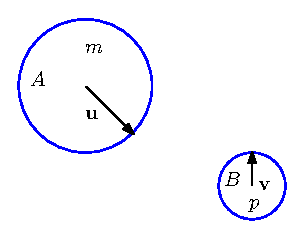
\includegraphics[width=1.2\textwidth]{img/02/colisionesAntes}
    \caption{Antes de la colisión.}
    \label{fig:coliAntes}
  \end{subfigure}
  \hspace{2cm}
  \begin{subfigure}[b]{0.32\textwidth}
    \includegraphics[width=0.75\textwidth]{img/02/colisionesDetecta}
    \caption{Colisión detectada}
    \label{fig:coliDetecta}
  \end{subfigure}
\\
\vspace{1cm}
  \begin{subfigure}[b]{0.32\textwidth}
    \includegraphics[width=0.8\textwidth]{img/02/colisionesResponde}
    \caption{Respuesta a la colisión.}
    \label{fig:coliResponde}
  \end{subfigure}
  \hspace{2cm}
  \begin{subfigure}[b]{0.32\textwidth}
    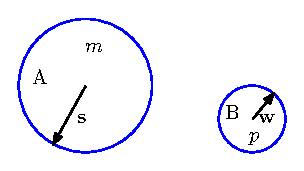
\includegraphics[width=1.1\textwidth]{img/02/colisionesAjusta}
    \caption{Después de la colisión}
    \label{fig:coliAjusta}
  \end{subfigure}
 \caption[Colisión elástica]{Etapas de detección y respuesta a una colisión} 
 \label{colision:fig}
\end{figure}

Suponemos también que conocemos todas las propiedades de los cuerpos, es decir su masa, su velocidad y su posición.

Queremos determinar una nueva posición y una nueva velocidad para los objetos como resultado de la colisión entre ellos (Figura~\ref{fig:coliAjusta}).
Esto se resume en el Cuadro~\ref{condiciones:Colision}.

\begin{table}
\ra{1.2}
\begin{center}
\begin{tabular} {@{}lll@{}}
\toprule
Objeto & Información conocida & Información por determinar \\
\midrule
$A$ & Masa $m$, Velocidad $\textbf{u}$ & Velocidad ajustada $\textbf{s}$ \\
$B$ & Masa $p$, Velocidad $\textbf{v}$ & Velocidad ajustada $\textbf{w}$ \\
\bottomrule
\end{tabular}
\end{center}
\caption{Condiciones de la respuesta a las colisiones}
\label{condiciones:Colision}
\end{table}

Para entender el porqué de la respuesta a la colisión, es necesario seguir los siguientes pasos\footnote{Esta es una reproducción del procedimiento mostrado en~\cite{FisicaMatematicasVideojuegos} con mi nomenclatura}.
Primero vamos por el caso más simple: dos objetos $A$ y $B$, con velocidades $\textbf{u}$ y $\textbf{v}$ respectivamente chocan, como respuesta a la colisión las velocidades de ambos objetos cambian a $\textbf{s}$ y $\textbf{w}$.
Ver la Figura~\ref{colision:fig}.

Suponemos que: $\textbf{v} = \textbf{0}$. Es decir el cuerpo $B$ no se mueve, está detenido esperando la colisión del cuerpo $A$. Sabemos que tenemos un vector $\vec{\textbf{n}}$ normal al plano de colisión.
Con este vector podemos dividir los demás vectores en una parte normal al plano y otra tangencial  (Figura~\ref{comVec:fig}), es decir:

\begin{figure}
 \centering
 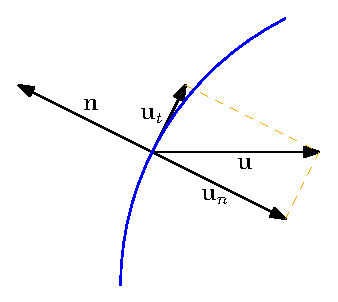
\includegraphics[width=7cm]{img/02/vector_componente}
 \caption[Separar componente tangencial y normal de un vector]{ 
 El vector $\textbf{u}$ se separa con respecto a $\textbf{n}$ en dos vectores uno normal $\textbf{u}_n$, y uno tangencial $\textbf{u}_t$ 
 } \label{comVec:fig}
\end{figure}

\begin{eqnarray}
 \textbf{u} & = & \textbf{u}_t + \textbf{u}_n \nonumber \\
 \textbf{v} & = & \textbf{v}_t + \textbf{v}_n \nonumber \\
 \textbf{s} & = & \textbf{s}_t + \textbf{s}_n \nonumber \\
 \textbf{w} & = & \textbf{w}_t + \textbf{w}_n \nonumber
\end{eqnarray}

Ahora veamos qué es lo qué sabemos de antemano por la forma como planteamos las condiciones del problema: sabemos que: $\textbf{u}_t = \textbf{s}_t$ y $\textbf{v}_t = \textbf{w}_t = \textbf{0}$, porque esperaríamos que las velocidades sólo se vieran afectadas en su componente normal y porque sabemos que el objeto $B$ estaba inicialmente en reposo.
Así que lo único que necesitamos saber es $\textbf{s}_n$ y $\textbf{w}_n$.

Se sabe también que, como la colisión es elástica, debe de obedecer la ley de la conservación de la energía~\eqref{eq:energia} y la la ley de la conservación de momento~\eqref{eq:momento}.

\begin{equation}
m \textbf{u}_n = m \textbf{s}_n + p \textbf{w}_n
\label{eq:momento}
\end{equation}

\begin{equation}
\frac{1}{2} m \textbf{u}^2 = \frac{1}{2} m \textbf{s}^2 + \frac{1}{2} p \textbf{w}^2
\label{eq:energia}
\end{equation}

Así que tenemos justo las condiciones necesarias para encontrar una solución, pues tenemos dos valores por determinar y dos ecuaciones que las relacionan.
Para encontrar la solución hacemos un cambio de variable $r = \frac{m}{p}$.
Podemos encontrar una expresión para $\textbf{w}_n$ de la ecuación~\eqref{eq:momento}, y lo sustituimos en~\eqref{eq:energia} para obtener el valor de $\textbf{s}_n$. En realidad se obtienen dos valores $\textbf{s}_{n}^{1} = \textbf{u}_n$ y $\textbf{s}_{n}^{2} = \textbf{u}_n \frac{r-1}{r+1}$, tomamos el segundo (el primero corresponde a la condición inicial, por que las colisiones elásticas son reversibles en el tiempo), y lo sustituimos de nuevo en~\eqref{eq:momento} para obtener el valor de $\textbf{w}_n = \frac{2 r \textbf{u}_n}{r + 1}$.

Con esto se tiene todo lo necesario  para resolver una colisión elástica con uno de los dos objetos en reposo. Podemos utilizar el siguiente pseudocódigo:

{\centering
\begin{minipage}{\linewidth}
  \begin{algorithm}[H]
    \caption{Respuesta a una colisión elástica}
    \label{alg:elas}
    \begin{algorithmic}[1] % The number tells where the line numbering should start 0 for no number
\Procedure{RespuestaColisionElastica}{$\textbf{u}, \textbf{n}, m, p$}
\State $r \gets \frac{m}{p}$
\State $\textbf{u}_n \gets$ \Call{parteNormal}{$\textbf{u}, \textbf{n}$}
\State $\textbf{u}_t \gets \textbf{u} - \textbf{u}_n$
\State $\textbf{s}_n \gets \textbf{u}_n \left( \frac{r - 1}{r + 1} \right) $
\State $\textbf{w}_n \gets \textbf{u}_n \left( \frac{2r}{r + 1} \right) $
\State $\textbf{s} \gets \textbf{u}_t + \textbf{s}_n$
\State $\textbf{w} \gets \textbf{w}_n$
\State \Return{$\textbf{s}, \textbf{w}$}
\EndProcedure
\Procedure{parteNormal}{$\textbf{v}, \textbf{n}$}
\State $\textbf{v}_n \gets \frac{(\textbf{v} \cdot \textbf{n})}{|\textbf{n}|} \frac{\textbf{n}}{|\textbf{n}|}$
\State \Return{$\textbf{v}_n$}
\EndProcedure
    \end{algorithmic}
  \end{algorithm}
\end{minipage}
\par
}

En donde la función \mintinline{cpp}{parteNormal}, es una función que recibe un vector $\textbf{u}$ y un vector $\textbf{n}$, devuelve la parte normal de $\textbf{u}$ con respecto a $\textbf{n}$.
Es decir, nos sirve para partir al vector $\textbf{u}$ en una parte tangencial y una parte normal a la colisión haciendo uso de las fórmulas \eqref{eq:sepVector}.

Ahora veamos el caso más general, donde $\textbf{v} \neq \textbf{0}$. Aquí vamos a ocupar el principio de relatividad y le restamos a todo el sistema $\textbf{v}$, lo que lo transforma en el caso anterior. Resolvemos como lo habíamos hecho antes y luego le sumamos a todo el sistema $\textbf{v}$. El pseudocódigo es casi idéntico:
 
{\centering
\begin{minipage}{\linewidth}
  \begin{algorithm}[H]
    \caption{Respuesta a una colisión elástica con ambos cuerpos en movimiento}
    \label{alg:elasmov}
    \begin{algorithmic}[1] % The number tells where the line numbering should start 0 for no number
\Procedure{RespuestaColisionElastica}{$\textbf{u}, \textbf{v}, \textbf{n}, m, p$}
\State $r \gets \frac{m}{p}$
\State $\textbf{u} \gets \textbf{u} - \textbf{v}$
\State $\textbf{u}_n \gets$ \Call{parteNormal}{$\textbf{u}, \textbf{n}$}
\State $\textbf{u}_t \gets \textbf{u} - \textbf{u}_n$
\State $\textbf{s}_n \gets \textbf{u}_n \left( \frac{r - 1}{r + 1} \right) $
\State $\textbf{w}_n \gets \textbf{u}_n \left( \frac{2r}{r + 1} \right) $
\State $\textbf{s} \gets \textbf{u}_t + \textbf{s}_n + \textbf{v}$
\State $\textbf{w} \gets \textbf{w}_n + \textbf{v}$
\State \Return{$\textbf{s}, \textbf{w}$}
\EndProcedure
    \end{algorithmic}
  \end{algorithm}
\end{minipage}
\par
}

Con esto podemos programar un función general que resuelva colisiones elásticas, sólo debemos asegurarnos de que la función que detecta las colisiones le informe a aquella función de tres cosas: las propiedades del objeto $A$, las propiedades del objeto $B$ y un vector normal al plano de colisión que vaya de $A$ a $B$.

Vuelvo a hacer énfasis en que para nuestro caso, la colisión de cada partícula con la esfera debe resolverse de manera separada e independiente.

\subsubsection{Colisiones inelásticas}
En una colisión inelástica se tiene una pérdida de energía como respuesta al impacto.
En la realidad las colisiones son inelásticas, podemos apreciar parte de la pérdida de la energía, al escuchar el sonido de la colisión.
Por ejemplo en el billar.

Para simular una colisión inelástica, vamos también a hacer una suposición: que los objetos tienen una cierta eficiencia, y que ésta se mantiene fija para todas las colisiones que involucran ese objeto.
Es una gran simplificación porque en la realidad la eficiencia de una colisión depende de muchos factores, como el medio ambiente, o la velocidad de los objetos al momento de la colisión.

Si dos objetos chocan y uno de ellos tiene \emph{coeficiente de restitución} de 0.9 y el otro un coeficiente de restitución de 0.85, la energía total después de la colisión sería: $\left( \text{0.9} \cdot \text{0.85} \right) \left(  E_b + E_a \right)$.
Donde $E_a$ y $E_b$ es la energía de cada objeto antes de la colisión.
Como se puede ver, el coeficiente de restitución es una manera de medir la \emph{eficiencia} y significa que el primer objeto después de una colisión transmite por ejemplo el 95 por ciento de su energía.

Para resolver una colisión inelástica se usa el mismo procedimiento que en la sección anterior, sólo que ahora la ecuación~\eqref{eq:energia}, toma la siguiente forma:
\begin{equation}
 \frac{1}{2} e m \textbf{u}^2 = \frac{1}{2} m \textbf{s}^2 + \frac{1}{2} p \textbf{w}^2
 \label{eq:energiaIne} 
\end{equation} 

Donde $e$ es el producto de los coeficientes de restitución de ambos objetos. Y se procede de la misma manera que en el caso anterior a calcular los valores de $\textbf{w}_n$ y $\textbf{s}_n$. Resolviendo el sistema formado por las ecuaciones~\eqref{eq:momento} y~\eqref{eq:energiaIne}.

Las nuevas soluciones son: 
\begin{eqnarray}
\textbf{s}_n & = & \frac{-r\textbf{u} - \sqrt{r^{2} \textbf{u}_{n}^{2} - \left( r + 1\right)  \left( (r - e) \textbf{u}_{n}^{2} + (1 -e) \textbf{u}_{t}^{2} \right) } } { r + 1} \nonumber \\
\textbf{w}_n & = & r \left(  n \textbf{u}_n - \textbf{v}_n \right) \nonumber
\end{eqnarray}

Y el pseudocódigo, que resuelve la colisión de manera inelástica es el siguiente:

{\centering
\begin{minipage}{\linewidth}
  \begin{algorithm}[H]
    \caption{Respuesta general a una colisión inelástica}
    \label{alg:inelas}
    \begin{algorithmic}[1] % The number tells where the line numbering should start 0 for no number
\Procedure{RespuestaColisionInelastica}{$\textbf{u}, \textbf{v}, \textbf{n}, m, p, E_a, E_b$}
\State $r \gets \frac{m}{p}$
\State $e \gets E_a \cdot E_b$
\State $\textbf{u} \gets \textbf{u} - \textbf{v}$
\State $\textbf{u}_n \gets$ \Call{parteNormal}{$\textbf{u}, \textbf{n}$}
\State $\textbf{u}_t \gets \textbf{u} - \textbf{u}_n$
\State $ d \gets r^{2} \left(  \textbf{u}_n \cdot \textbf{u}_n \right) - \left( (r - e) (\textbf{u}_n \cdot \textbf{u}_n) + (1 - e) (\textbf{u}_t \cdot \textbf{u}_t) \right) $
\State $\textbf{s}_n \gets \textbf{n} \left( \frac{ \sqrt{d} - r \textbf{u}_n }{r + 1} \right) $
\State $\textbf{w}_n \gets r \left( \frac{\textbf{u}_n - \textbf{v}_n}{r + 1} \right) $
\State $\textbf{s} \gets \textbf{u}_t + \textbf{s}_n + \textbf{v}$
\State $\textbf{w} \gets \textbf{w}_n + \textbf{v}$
\State \Return{$\textbf{s}, \textbf{w}$}
\EndProcedure
    \end{algorithmic}
  \end{algorithm}
\end{minipage}
\par
}


\chapter{Implementación del modelo}
Este capítulo está dedicado a cubrir los detalles de la implementación del modelo en código, concretamente en lenguaje C++.

Dado que la principal finalidad de este trabajo es el modelado físico, no entraré en detalles en otras áreas del programa más que las que tienen que ver con lo descrito en los capítulos anteriores.

El programa completo contiene módulos para la graficación en \href{http://www.opengl.org/}{OpenGL}, para la interfaz de usuario por medio de \href{https://github.com/ocornut/imgui}{dear imgui}, para la lectura y escritura de imágenes usando \href{http://freeimage.sourceforge.io/}{freeimage} (para cargar texturas y para hacer capturas de pantalla) e implementa el modelo de iluminación de \href{http://en.wikipedia.org/wiki/Phong_reflection_model}{Phong} en shaders por medio de \href{http://www.khronos.org/opengl/wiki/OpenGL_Shading_Language}{GLSL}.

El lector interesado puede consultar el código fuente completo del programa que se incluye en un CD o puede descargarlo de \href{http://github.com/nemediano}{github}.
Aunque el código está escrito en inglés (por ser el estándar) traté de ser lo más extenso en los comentarios en todo el código.
Por lo que el lector que cuente con los conocimientos de programación y graficación por computadora adquiridos en la licenciatura podrá entender y usar todo el código fuente del programa sin ningún problema.

Se decidió implementar el programa usando el paradigma de programación orientada a objetos. 
En la primera sección se describen las clases más importantes: las necesarias para representar las estructuras del modelo y la clase que representa el cuerpo neumático.

La siguiente sección se revisa cómo se implementaron en código los métodos numéricos usados para integrar la ecuación de Newton.

En la tercera sección se explican las rutinas de la física del modelo, concretamente las rutinas que se encargan de aplicar las fuerzas que intervienen en el modelo.

En la última sección del capítulo, se explica cómo es que se implementaron la rutina tanto de detección como de respuesta a las colisiones.

\section{Diseño de clases}

\epigraph{\say{Show me your flowchart and conceal your tables, and I shall continue to be mystified. Show me your tables, and I won't usually need your flowchart; it'll be obvious.}}{\textit{Frederick P. Brooks \\ Mythical Man-Month}}

Decidí usar de la biblioteca de álgebra para gráficos \href{http://github.com/g-truc/glm}{glm} por dos razones:
Primero, porque cuenta con tipos de datos para representar vectores en 2 y 3 dimensiones e implementa las operaciones usuales entre ellos.
Y segundo, porque esta biblioteca tiene un alto nivel de integración con OpenGL al grado de ser casi un estándar.

La parte fundamental del modelo la constituyen las partículas; de cada una de éstas nos interesa saber básicamente cuatro cosas: su posición, su velocidad, la fuerza que se le está aplicando y la masa.
Adicionalmente, por un detalle particular a nuestra implementación, se necesita saber si una partícula está fija.
Si una partícula está fija, entonces se deben de ignorar las operaciones de integración.
La clase \mintinline{cpp}{Particle} representa (abstrae) una partícula. Los métodos nos permiten editar y consultar estos cinco miembros.
En este sentido la clase \mintinline{cpp}{Particle} es muy simple~\footnote{En el argot del lenguaje \href{http://www.java.com/en/}{Java} diriamos que la clase \mintinline{cpp}{Particle} es casi un \href{http://en.wikipedia.org/wiki/JavaBeans}{bean}}.

Para representar a los resortes-amortiguadores se creó la clase \mintinline{cpp}{SpringDamper} que tiene como miembros \emph{referencias} a las dos partículas que une éste resorte.
Hago énfasis en que usaremos referencias, pues las partículas van ser usadas para formar varios objetos y se requiere que no sea necesario actualizar en cada objeto por separado cada que una partícula sea modificada. Finalmente, se debe saber la longitud $L$ del resorte cuando está en su estado de reposo.

La clase \mintinline{cpp}{SpringDamper} define los métodos para:
\begin{itemize}
 \item Actualizar qué partículas forman éste resorte.
 \item Consultar y modificar $L$.
 \item Consultar las posiciones de las partículas que forman éste resorte.
 \item Acumular la fuerza del resorte en sus dos partículas dados $k_s$ y $k_d$.
\end{itemize}

La última clase necesaria para definir el cuerpo neumático es la clase \mintinline{cpp}{Face}, que representa una cara del cuerpo flexible.
Como es de esperar, dado que las caras son cuadriláteros, esta clase solo necesita como propiedades referencias a cuatro partículas.

Adicionalmente, la clase \mintinline{cpp}{Face} implementa los siguientes métodos:
\begin{itemize}
 \item Los accesores y mutadores a las partículas que la forman.
 \item Un método para actualizar las partículas que forman esta cara (equivalente al de \mintinline{cpp}{SpringDamper}).
 \item Un método para calcular el área de esta cara.
 \item Un método que sirve como auxiliar en el cálculo del volumen de todo el cuerpo flexible. La lógica de este método se explica en la Sección~\ref{sec:fuerzaGas}.\footnote{Aunque ésta no es estrictamente hablando una propiedad de la cara, por razones de Ingeniería de Software (IS) era conveniente incluirlo en esta clase.}
\end{itemize}

La clase que representa el cuerpo flexible: \mintinline{cpp}{SoftBody} está compuesta con objetos de las clases anteriores.
Esta clase es la más importante de la aplicación.
Y el resto de éste capítulo está dedicado a explicar como funcionan sus métodos.
En este momento, es relevante decir que esta clase contiene una colección de partículas, una colección de resortes y una colección de caras.
Las caras y resortes en realidad usan (agregan) referencias a las partículas, de esta manera la información de las partículas sólo está almacenada una vez.

Por orden, esta clase también define una estructura: \mintinline{cpp}{SoftBodyParameters} que contiene todos los parámetros físicos del cuerpo flexible. 
 
Finalmente, se necesita también una clase para representar el único cuerpo rígido en la escena.
La clase \mintinline{cpp}{Ball} tiene como miembros una partícula, un escalar que representa el radio de la esfera y un miembro para registrar qué método numérico se usa para integrar.\footnote{De nuevo por IS, era conveniente que cada objeto en la escena llevará registro de que integrador está en uso}

La relación entre estas clases está resumida en el diagrama de clases mostrado en la Figura~\ref{clases:fig}. De nuevo hago énfasis en que la implementación de contiene de hecho más miembros que los mostrados en dicha figura, pues solo aparecen en el diagrama los relevantes para éste trabajo.

\begin{figure}
 \centering
 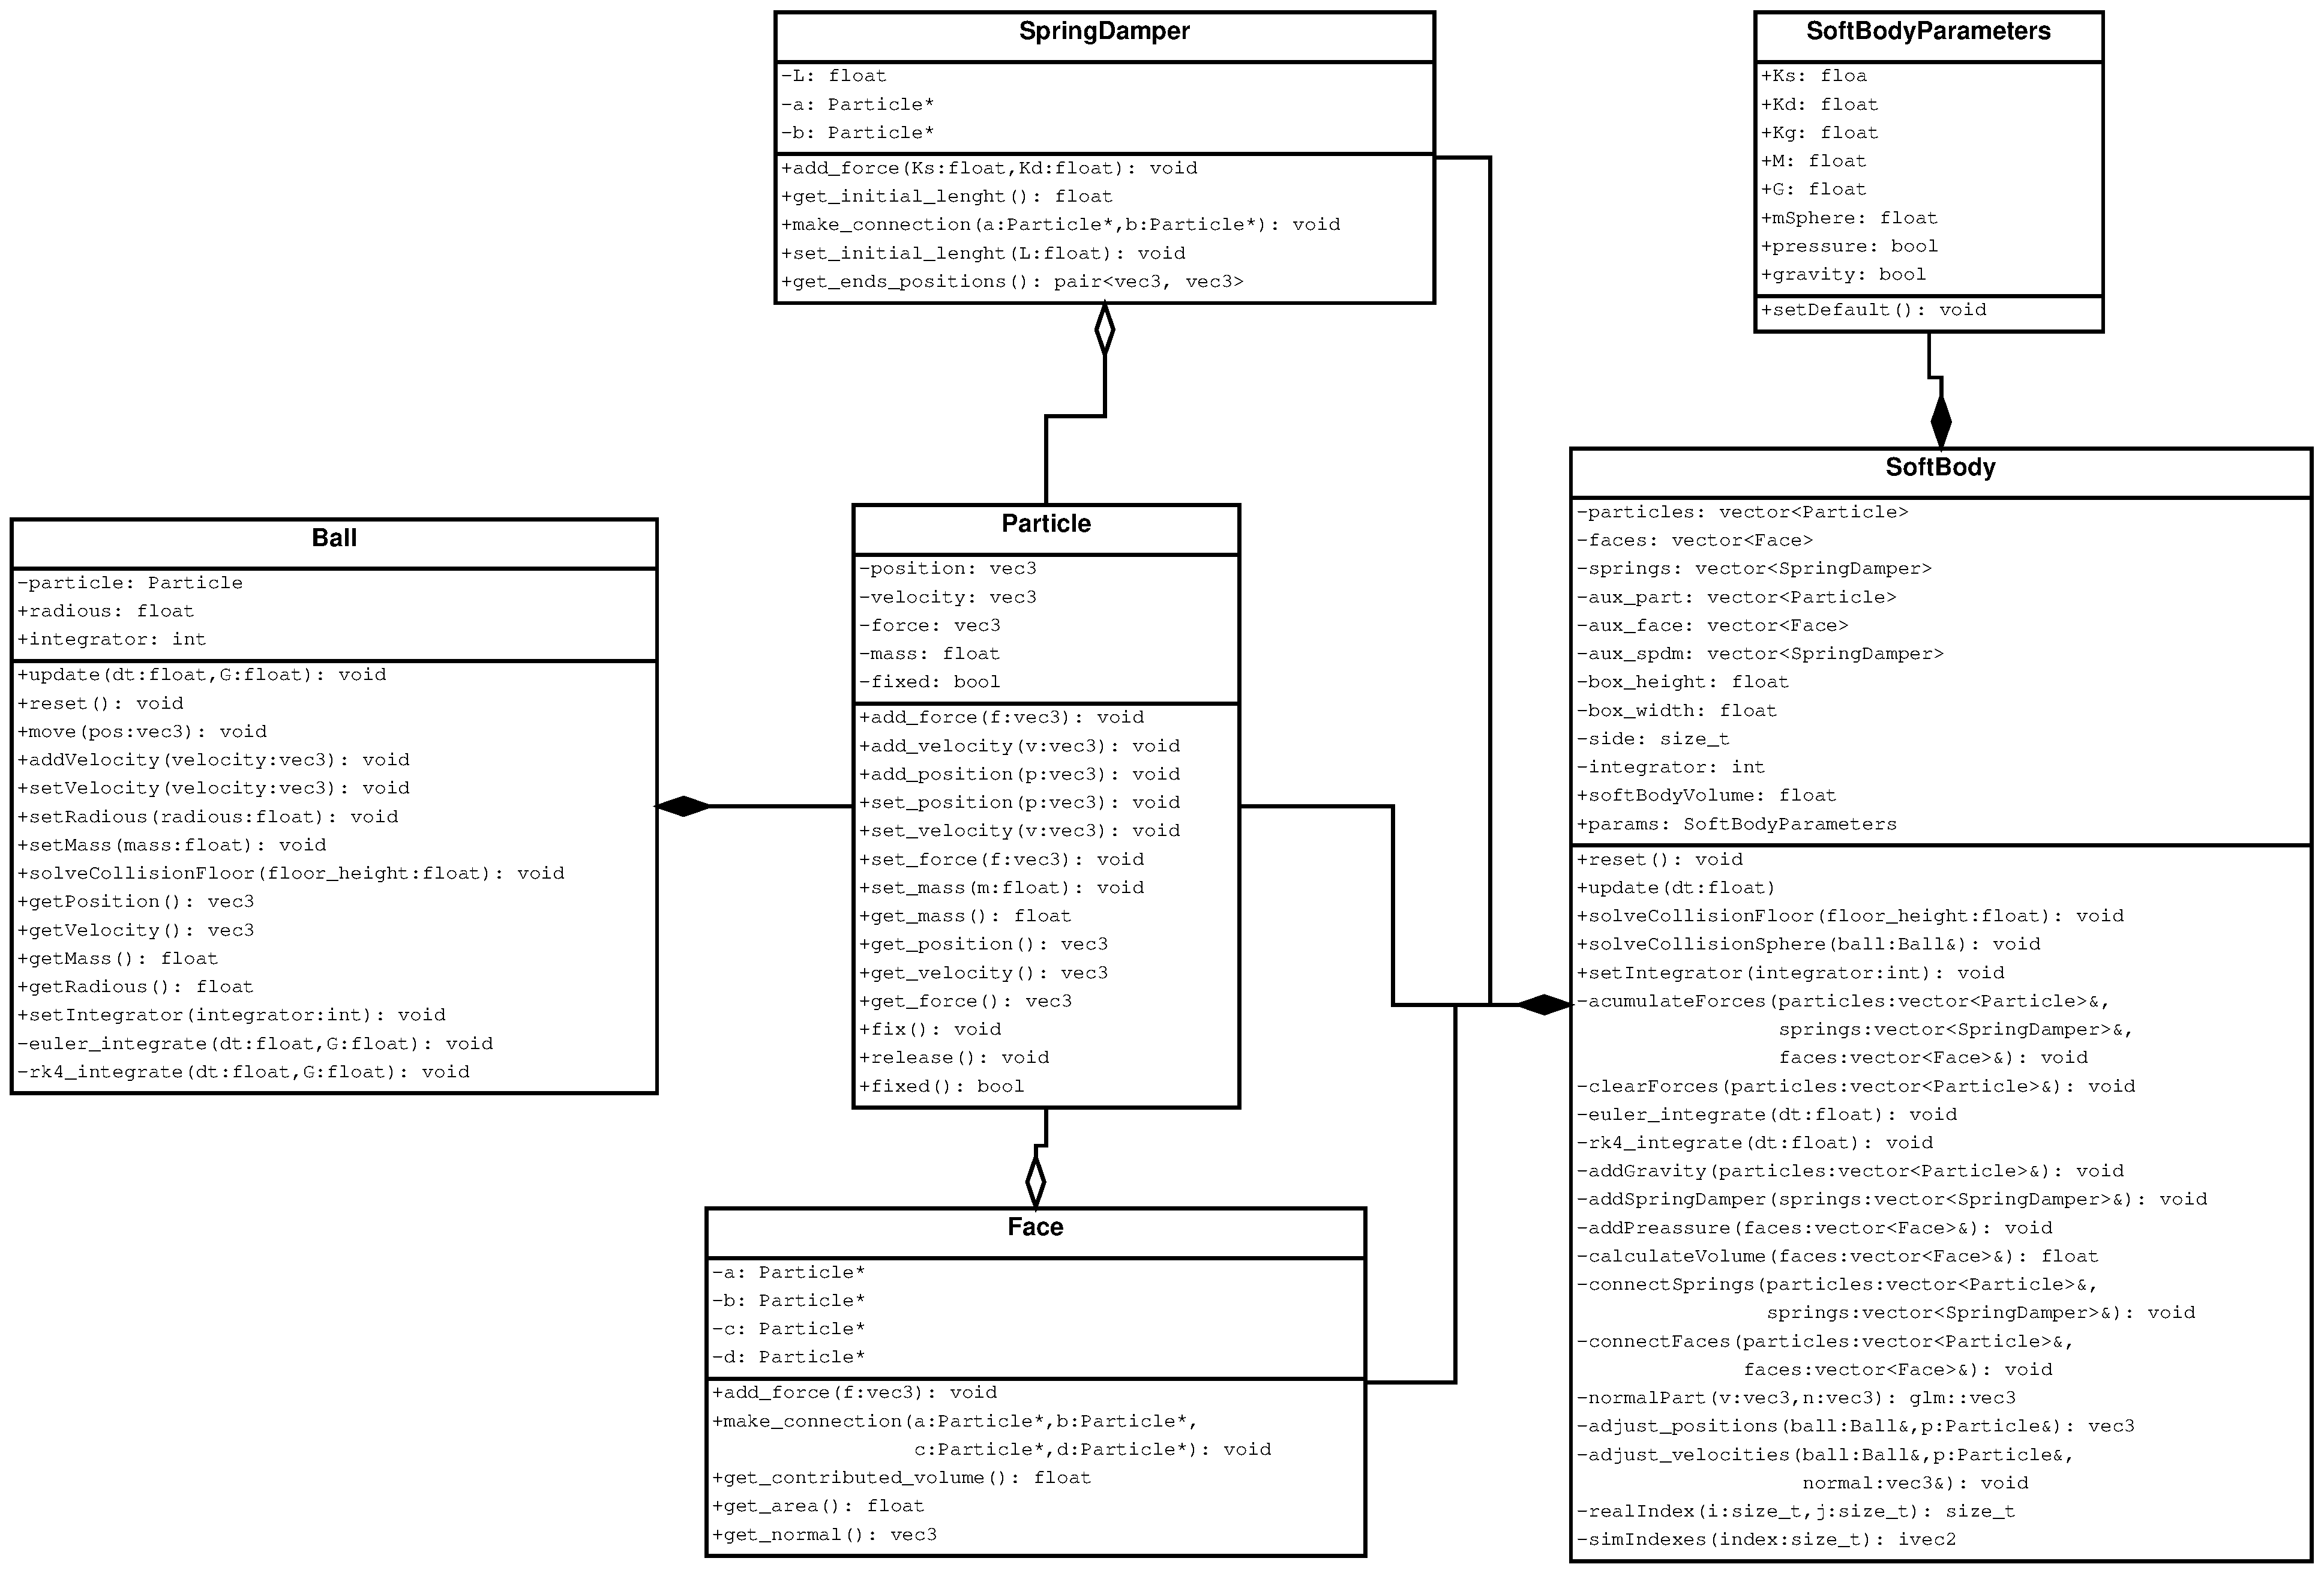
\includegraphics[width=\textwidth]{img/03/diagramaClases}
 \caption[Diagrama de clases]{ 
 La clase \mintinline{cpp}{Particle} es la unidad de construcción. La clase \mintinline{cpp}{SoftBody} es el objeto principal que contiene a los demas. 
 } \label{clases:fig}
\end{figure}

\section{Creación del cuerpo flexible}

Cómo se dijo en la sección anterior, hay tres colecciones que forman el cuerpo flexible: las partículas, los resortes y las caras.
Estas colecciones están almacenadas en arreglos dinámicos\footnote{En lenguaje C++ representados por objetos de tipo \mintinline{cpp}{std::vector}, los llamo \emph{colecciones} en el texto para no confundirlos con los vectores de álgebra lineal} que forman parte de la clase \mintinline{cpp}{SoftBody}.

Hay algunas cosas que decir aquí: primero, que lo que se quiere modelar es una tela cuadrada que servirá como cuerpo flexible, por lo que el número de partículas es en realidad $n^{2}$ en donde $n$ es el número de puntos en cada lado de la tela (en el código, $n$ es el miembro \mintinline{cpp}{m_side} de \mintinline{cpp}{SoftBody}), y como no hay resortes en las orillas de la tela el número de resortes totales es $2 (n - 1) (n - 2)$ y el número de caras es: $(n-1)^{2}$.
Segundo, que pese a que geométricamente la tela es un arreglo cuadrado de puntos, las partículas son guardados en un arreglo unidimensional (lineal), dado que esto  simplifica y hace mucho más generales las rutinas de acumulación de fuerza.

Dado que la partículas están en un arreglo unidimensional se hace uso del método \mintinline{cpp}{simIndexes} que recibe el índice de la partícula en el vector unidimensional y nos regresa los índices $(i, j)$ que la partícula tendría en un arreglo bidimensional. El método \mintinline{cpp}{realIndex} hace la operación inversa.

\begin{listing}
\inputminted[
  firstline=303, %If you omit this two fields, the whole file is pulled
  lastline=341
  ]{cpp}{../programa/physics/SoftBody.cpp}
  \caption{El método \mintinline{cpp}{recreate_particles} de \mintinline{cpp}{SoftBody}}\label{lst:recreate_particles}
\end{listing}

El código mostrado en el Listado~\ref{lst:recreate_particles} inicializa la velocidad, la fuerza y la masa de la partículas (la posición es inicializada con una rutina muy simple que está fuera de la clase \mintinline{cpp}{SoftBody}). 
También se encarga de fijar las partículas que están en las orillas de la tela.

La rutina que inicializa los resortes es ejecutada después que la de las partículas. Se muestra un extracto en el Listado~\ref{lst:connectSprings}.

\begin{listing}
\inputminted[
  firstline=343, %If you omit this two fields, the whole file is pulled
  lastline=371
  ]{cpp}{../programa/physics/SoftBody.cpp}
  \caption{El método \mintinline{cpp}{connectSprings} de \mintinline{cpp}{SoftBody}}\label{lst:connectSprings}
\end{listing}

Por las condiciones que definimos en nuestra tela.
\begin{itemize}
 \item Las partículas que están en las aristas superiores e inferiores de la tela no tienen un resorte horizontal entre ellas.
 \item Las partículas que están en las aristas izquierda y derecha de la tela no tienen un resorte vertical entre ellas.
\end{itemize}

El algoritmo, pregunta si esta partícula puede ser unida (por un resorte) con la partícula a su derecha, de ser así las conecta. Después, pregunta si debe ser unida con la partícula debajo de ella, de ser así también es conectada.

\begin{listing}
\inputminted[
  firstline=373, %If you omit this two fields, the whole file is pulled
  lastline=392
  ]{cpp}{../programa/physics/SoftBody.cpp}
  \caption{El método \mintinline{cpp}{connectFaces} de \mintinline{cpp}{SoftBody}}
  \label{lst:connectFaces}
\end{listing}

La lógica para formar las caras se presenta en el Listado~\ref{lst:connectFaces}.
Esta rutina es muy parecida a la anterior: recorre todas las partículas, si la partícula actual, tiene un partícula a su izquierda y otra partícula abajo, entonces se pueden tomar cuatro partículas (pues debe existir otra una partícula en diagonal) para formar una cara.

\section{La física del modelo}
Toca el turno de ver las rutinas que tienen que ver con la acumulación de fuerzas en el modelo.
Como se ha dicho antes hay básicamente tres fuerzas que se deben acumular, la de la gravedad, la de los resortes amortiguadores y la debida a la presión del gas.

Aquí es donde empezaremos a notar el porqué de la construcción de los demás vectores de referencias.

\subsection{La fuerza de gravedad}
La primera y más sencilla de las fuerzas que vamos a poner es la de gravedad.
Como se dijo desde la ecuación~\eqref{fuerzaGravedad}, sólo depende de dos cosas de la masa del objeto y de la constante de gravedad\footnote{La contribución de la masa será \emph{cancelada} por el integrador}, y además sólo afecta el componente vertical (paralelo al eje $y$), del vector fuerza.

La fuerza de gravedad se aplica a cada una de las partículas del cuerpo flexible. 
Convenientemente, tenemos un vector con dichas partículas.
Por lo anterior y gracias a que glm sobrecarga los operadores en vectores de la manera natural, la implementación es trivial como se puede ver en el Listado~\ref{lst:addGravity}.
La constante de gravedad es un miembro de \mintinline{cpp}{SoftBody} y tiene el signo negativo.

Para hacer posible el analisis de la Sección~\ref{sec:performance}, se hacen uso de cronómetros. La estructura \mintinline{cpp}{mTimers} contiene estos cronómetros  y el Listado~\ref{lst:addGravity} es un claro ejemplo de su uso. Estos cronómetros son una forma muy simplista de \emph{instrumentación} de un método.

\begin{listing}
\inputminted[
  firstline=589, %If you omit this two fields, the whole file is pulled
  lastline=598
  ]{cpp}{../programa/physics/SoftBody.cpp}
  \caption{El método \mintinline{cpp}{addGravity} de \mintinline{cpp}{SoftBody}}
  \label{lst:addGravity}
\end{listing}

\subsection{La fuerza de los resortes}

La implementación de estos métodos también es trivial gracias a nuestro diseño.
Tan solo se debe iterar por todos los resortes de \mintinline{cpp}{SoftBody} en cada resorte se debe ocupar la ecuación~\eqref{fuerzaResorte}, para acumular la fuerza en los dos puntos que son unidos por ese resorte (Listado~\ref{lst:addSpringDamper}).
Solo por completez, en Listado~\ref{lst:add_forceSD} se muestra el método \mintinline{cpp}{add_force} de \mintinline{cpp}{SpringDamper} que en esencia implementa la ecuación~\eqref{fuerzaResorte}.

\begin{listing}
\inputminted[
  firstline=600, %If you omit this two fields, the whole file is pulled
  lastline=607
  ]{cpp}{../programa/physics/SoftBody.cpp}
  \caption{El método \mintinline{cpp}{addSpringDamper} de \mintinline{cpp}{SoftBody}}
  \label{lst:addSpringDamper}
\end{listing}

\begin{listing}
\inputminted[
  firstline=19, %If you omit this two fields, the whole file is pulled
  lastline=32
  ]{cpp}{../programa/physics/SpringDamper.cpp}
  \caption{El método \mintinline{cpp}{add_force} de \mintinline{cpp}{SpringDamper}}
  \label{lst:add_forceSD}
\end{listing}

\subsection{La fuerza del gas}
\label{sec:fuerzaGas}

La siguiente fuerza en ser acumulada es la fuerza debida a la presión del gas. Para esto se ocupa la ecuación~\eqref{fuerzaGas}, y se debe de acumular en cada cara.
Para poder calcular esta fuerza se necesitan hacer varias operaciones importantes: calcular el volumen total del cuerpo flexible y además calcular el área y el vector normal de cada una de las caras (Listado~\ref{lst:addPreassure}).

\begin{listing}
\inputminted[
  firstline=609, %If you omit this two fields, the whole file is pulled
  lastline=623
  ]{cpp}{../programa/physics/SoftBody.cpp}
  \caption{El método \mintinline{cpp}{addPreassure} de \mintinline{cpp}{SoftBody}}
  \label{lst:addPreassure}
\end{listing}

Para hacer el cálculo de volumen se hace uso de la ecuación~\eqref{eq:volumen}.
Hay que recordar que el cuerpo neumático está formado por seis caras.
Cinco de las cuales están fijas y otra es la tela (o tapa) que es el cuerpo flexible.
Cada cara es dividida en dos triángulos para calcular su contribución al volumen.
El Listado~\ref{lst:calculateVolume} muestra la lógica. La función \mintinline{cpp}{tethVolume} implementa las ecuaciones~\eqref{eq:baricentro} y~\eqref{eq:normTriag} y por completez se muestra en el Listado~\ref{lst:calculateTethVolume}.

\begin{listing}
\inputminted[
  firstline=625, %If you omit this two fields, the whole file is pulled
  lastline=660
  ]{cpp}{../programa/physics/SoftBody.cpp}
  \caption{El método \mintinline{cpp}{calculateVolume} de \mintinline{cpp}{SoftBody}}
  \label{lst:calculateVolume}
\end{listing}

\begin{listing}
\inputminted[
  firstline=35, %If you omit this two fields, the whole file is pulled
  lastline=41
  ]{cpp}{../programa/math/mathhelpers.cpp}
  \caption{La función \mintinline{cpp}{tethVolume} implementa parte de la ecuación~\eqref{eq:volumen}}
  \label{lst:calculateTethVolume}
\end{listing}

El método \mintinline{cpp}{calculateVolume} de la clase \mintinline{cpp}{Face}, suma la contribución de una cara al volumen usando la misma función \mintinline{cpp}{tethVolume} dos veces en los puntos que forman la cara (Listado~\ref{lst:get_contributed_volume})

\begin{listing}
\inputminted[
  firstline=65, %If you omit this two fields, the whole file is pulled
  lastline=73
  ]{cpp}{../programa/physics/Face.cpp}
  \caption{El método \mintinline{cpp}{get_contributed_volume} de \mintinline{cpp}{Face}}
  \label{lst:get_contributed_volume}
\end{listing}

Para calcular el área de cada cara se ocupa la fórmula~\eqref{formulaArea}, como se puede ver en el Listado~\ref{lst:get_area}.
Y para calcular el vector normal se hace uso de la fórmula~\eqref{formulaVecNormal}, en donde $n=4$, dado que cada cara está formada por cuatro puntos (Listado~\ref{lst:get_normal}).

\begin{listing}
\inputminted[
  firstline=44, %If you omit this two fields, the whole file is pulled
  lastline=53
  ]{cpp}{../programa/physics/Face.cpp}
  \caption{El método \mintinline{cpp}{get_area} de \mintinline{cpp}{Face}}
  \label{lst:get_area}
\end{listing}

\begin{listing}
\inputminted[
  firstline=55, %If you omit this two fields, the whole file is pulled
  lastline=63
  ]{cpp}{../programa/physics/Face.cpp}
  \caption{El método \mintinline{cpp}{get_normal} de \mintinline{cpp}{Face}}
  \label{lst:get_normal}
\end{listing}

\section{Los métodos numéricos}
Otras de las rutinas complicadas son los métodos numéricos.
Para integrar la ecuación de Newton, se requiere saber la posición y la velocidad actual de cada una de las partículas del modelo y tener una manera de llamar a la función que se encarga de acumular las fuerzas.

\subsection{El método de Euler}
Básicamente se trata de tomar las ecuaciones~\eqref{formulas:Euler} e implementarlas en el código (Listado~\ref{lst:euler_integrate}), aprovechando la gran ventaja de que el método de Euler puede integrar una partícula la vez.

\begin{listing}
\inputminted[
  firstline=466, %If you omit this two fields, the whole file is pulled
  lastline=477
  ]{cpp}{../programa/physics/SoftBody.cpp}
  \caption{El método \mintinline{cpp}{euler_integrate} de \mintinline{cpp}{SoftBody}}
  \label{lst:euler_integrate}
\end{listing}

\subsection{El método de Runge-Kutta}
Aquí se explica el que fue probablemente el método numérico más complicado de implementar, pues no tiene la ventaja de Euler de integrar cada partícula independientemente, así que necesita integrar todas juntas.
Además, debe tener espacio para guardar los ponderadores del paso de integración de cada partícula.

Para tener una idea clara de lo que que hace el código en el Listado~\ref{lst:rk4_integrate} conviene volver a ver las ecuaciones~\eqref{ponderadores:RK4} y~\eqref{formulas:RK4}.
Lo largo del proceso hacen ver el Listado~\ref{lst:rk4_integrate} un poco más complicado que lo que en realidad es.

\begin{mintedCode} %El codigo es muy largo, ocupo un ambiene no flotante
\inputminted[
  firstline=479, %If you omit this two fields, the whole file is pulled
  lastline=556
  ]{cpp}{../programa/physics/SoftBody.cpp}
  \caption{El método \mintinline{cpp}{rk4_integrate} de \mintinline{cpp}{SoftBody}}
  \label{lst:rk4_integrate}
\end{mintedCode}

El truco consiste en ocupar un conjunto de puntos, resortes y caras auxiliares, para con ellos evaluar la función fuerza que es necesaria para calcular los ponderadores del método de RK4 (Por eso están presentes en el diagrama de la Figura~\ref{clases:fig}), después la rutina es muy parecida a la de Euler.

\section{El manejo de las colisiones}
Como ya se ha dicho antes, el problema de las colisiones se resuelve en dos partes: primero la detección y luego la respuesta.
La forma de responder consiste básicamente en mover los objetos que se colisionan a un lugar donde ya no choquen y ajustar las velocidades como respuesta.

\subsection{La rutina de las colisiones}
La detección es llevada a cabo en dos funciones.
Recordemos que nuestra tarea de detección se simplifica muchísimo por el hecho de que uno de los objetos, el objeto incidente es una esfera.
Para saber si dicha esfera está en colisión con nuestro cuerpo flexible, lo que hacemos es probar si cualquiera de las partículas está dentro de la esfera; de ser así, empezamos a resolver la colisión entre la esfera y la partícula en cuestión. Después seguimos revisando el resto de las partículas.
El Listado~\ref{lst:solveCollisionSphere} implementa el algoritmo.

\begin{listing}
\inputminted[
  firstline=700, %If you omit this two fields, the whole file is pulled
  lastline=713
  ]{cpp}{../programa/physics/SoftBody.cpp}
  \caption{El método \mintinline{cpp}{solveCollisionSphere} de \mintinline{cpp}{SoftBody}}
  \label{lst:solveCollisionSphere}
\end{listing}

\subsection{La detección de la colisión}
El método del Listado~\ref{lst:adjust_positions} en se encarga de calcular el vector normal al lugar de la colisión y de mover el punto fuera de la esfera.
Mover el punto fuera de la esfera es en realidad parte de la respuesta a la colisión, pero decidí implementarlo en un solo método llamado \mintinline{cpp}{adjust_positions}, para que en la siguiente parte sólo se tenga que ajustar las velocidades.

\begin{listing}
\inputminted[
  firstline=715, %If you omit this two fields, the whole file is pulled
  lastline=728
  ]{cpp}{../programa/physics/SoftBody.cpp}
  \caption{El método \mintinline{cpp}{adjust_positions} de \mintinline{cpp}{SoftBody}}
  \label{lst:adjust_positions}
\end{listing}

El Listado~\ref{lst:adjust_positions}, primero calcula el vector normal que va del centro de la esfera a la partícula.
Luego, si la partícula no está fija, la mueve justo fuera de la esfera.
Si la partícula estuviera fija, lo que hace es mover a la esfera fuera de ella.

\subsection{La respuesta de la colisión}
La mayor parte del trabajo se hizo en la función anterior, ahora que sabemos el vector normal unitario: $\vec{\textbf{n}}$ a la colisión, el Listado~\ref{lst:adjust_velocities} solo se encarga de seguir los pasos explicados en el Algoritmo~\ref{alg:elasmov}.

\begin{listing}
\inputminted[
  firstline=730, %If you omit this two fields, the whole file is pulled
  lastline=745
  ]{cpp}{../programa/physics/SoftBody.cpp}
  \caption{El método \mintinline{cpp}{adjust_velocities} de \mintinline{cpp}{SoftBody}}
  \label{lst:adjust_velocities}
\end{listing}

Es importante que la velocidad y posición de la esfera sean ajustadas de manera independiente por cada partícula con la que se haya producido una colisión.
Es \emph{físicamente incorrecto} tratar de acumular las posiciones y velocidades de respuesta de colisión con cada partícula y luego actualizar el cuerpo rígido una sola vez con las resultantes.


\chapter{Diseño del experimento}
En este capítulo se analizan los resultados que se obtuvieron al haber implementado el modelo, y se divide en tres partes.
En la primera de ellas se cuenta cómo es que se decidió implementar el modelo, así como también cuales de sus variables se dejaron fijas (serían constantes en esta implementación) y cuáles es posible variar desde la interfaz de usuario.

En la segunda parte se diseñaron ciertas pruebas con el fin de poner en evidencia características particulares del modelo, específicamente su correcto comportamiento físico.

Y en la última parte se reportan los resultados de las pruebas de desempeño a las que se sometió el programa.

\section{Definición del sistema}
En esta primera parte presento el experimento y explico que parámetros fijé y cuáles pueden ser cambiados por el usuario.

\subsection{Características del modelo}
Tal como se explicó en la Sección~\ref{descripcion:experimento}, se modela un hexaedro regular, donde cinco de sus seis caras son rígidas y la cara superior o tapa es flexible: además, asumo que este hexaedro está relleno de gas.
En este sentido, el hexaedro completo (o caja) es el cuerpo neumático.
Mientras que la cara superior (o tela) es el cuerpo flexible.
Se deja caer sobre la tela una esfera rígida (o pelota).
Un ejemplo del programa terminado se muestra en la Figura~\ref{programa:portada}.
\begin{figure}
 \centering
 \includegraphics[width=0.85\textwidth]{img/04/modeloPortada}
 \caption[Ejemplo del programa en ejecución]{Una imagen del programa que implementa el modelo.}
 \label{programa:portada}
\end{figure}

\subsubsection{Constantes del experimento}
En una situación como la antes descrita hay muchísimas variables del modelo, sin embargo al momento de hacer la implementación en código decidí dejar fijas algunas de ellas, es decir que la única manera de cambiarlas es modificando en el código fuente y recompilando el programa por completo.
Aquí está la lista de estas variables y su significado.

Las variables que se decidieron dejar fijas, y que por ende se convierten en constantes en el experimento son las siguientes:

\begin{itemize}
 \item El número de partículas por lado de la tela.
 \item Las dimensiones (alto, ancho y largo) de la caja.
 \item La masa total de la tela. Y por lo tanto, la masa de cada partícula es ésta cantidad dividida entre el número total de partículas.
 \item El radio y la posición de la pelota.
 \item El tamaño del paso en el tiempo $\Delta t$ que se usa para los métodos numéricos de integración.
\end{itemize}

Los valores de estas constantes con las que se hizo este experimento están en el Cuadro~\ref{valores:constantes}.
\begin{table}
\ra{1.2}
\begin{center}
\begin{tabular} {@{}lrp{8cm}@{}}
\toprule
Constante & Valor & Comentario\\ 
\midrule
 Número de partículas & 22 & Para que se vea mejor el modelo, se elige un número par\\
 Dimensiones caja & $0.75 \times 1.5 \times 1.5$ & Se forma una caja de tapas cuadradas \\
 Masa tela & 10 & La masa de cada partícula es entonces $\frac{10}{22^{2}}$ \\
 Radio pelota & 0.25 &  \\
 Posición pelota & $(0, 1.5, 0)$& Como el cuerpo neumático está centrado en el origen. La pelota está justo arriba de él en el centro\\
 $\Delta t$ & 0.0025 & Determinado experimentalmente \\
\bottomrule
\end{tabular}
\caption[Valores de las constantes durante el experimento]{Valor de las constantes del experimento}
\label{valores:constantes}
\end{center}
\end{table}

\subsubsection{Variables físicas del experimento}
La variables físicas del experimento pueden ser modificadas en tiempo de ejecución por medio del menú que muestra en la Figura~\ref{programa:menu}.

\begin{figure}
 \centering
 \includegraphics[width=0.33\textwidth]{img/04/menu}
 \caption[Menú de usuario del programa]{Menú de usuario.}
 \label{programa:menu}
\end{figure}

Para la pelota o esfera (\emph{\textenglish{Sphere}}) que se refiere al cuerpo rígido.
la única variable que se puede modificar es su masa.

Los parámetros del cuerpo flexible que es posible modificar se dividen en tres subcategorias una por cada fuerza que se acumula.

La categoría del \emph{Gas}, al que se puede prender o apagar por medio del checkbox \emph{\textenglish{Pressure}}. 
Además, se puede modular su magnitud variando el valor de la constante $k_{g}$, por medio del control.

La de la \emph{\textenglish{Gravity}}, que al igual que la anterior se puede prender o apagar con el control  y también se puede modular variando el valor de la constante $g$.

La última subcategoria es la debida al resorte amortiguador (\emph{\textenglish{Spring-Damper}}.)
Esta fuerza no se puede apagar, pero se puede variar modificando dos parámetros $k_{s}$, que, como ya se dijo, controla la rigidez del resorte y $k_{d}$ que controla el amortiguamiento o pérdida de energía debida al resorte.

Aunque no es propiamente una opción de la física. El menú también permite elegir que método numérico usar para integrar.
Las opciones disponibles son: \emph{Euler} y \emph{Runge-Kutta}.

Los valores de default de estas variables (el valor que tiene al iniciar la ejecución) son los que muestra la Tabla~\ref{valores:variables}.

\begin{table}
\ra{1.2}
\begin{center}
%\begin{tabular} {|c|c|p{10cm}|}
\begin{tabular} {@{}llp{10cm}@{}}
\toprule
Parámetro & Valor & Comentario\\
\midrule
 Masa & 0.08 & Masa del cuerpo rígido \\
 Integrador & Runge-Kutta & Método Numérico con el que se integra. \\
 Gas & Activado & El programa empieza con la fuerza del gas prendida \\
 $k_g$ & 17 & Constante de presión del gas \\
 Gravedad & Activada & La gravedad está activada \\
 $g$ & -10.0 & La gravedad es negativa (jala hacia abajo) \\
 $k_s$ & 100 & La fuerza de los resortes \\
 $k_d$ & 5 & El valor de damping \\
\bottomrule
\end{tabular}
\end{center}
\caption[Valores por defecto de las variables físicas]{Valor inicial de los parámetros del experimento}
\label{valores:variables}
\end{table}

\subsubsection{Opciones de control y visualización}
Hay otras opciones que se pueden modificar por medio del menú, que se refieren más a cómo controlamos la animación y a como se ve el modelo que a la física.

Dentro de las del flujo de la animación, sólo hay dos controles, el de \emph{\textenglish{Pause/Play}}, que puede detener (reanudar) la animación física (se sigue pudiendo mover la cámara).
Y el botón de \emph{\textenglish{Reset}}, que devuelve a todos los objetos a su posición original.

El botón de \emph{\textenglish{Drop}}, hace que la esfera se deje caer.

Dentro de la categoría de \emph{\textenglish{Render}}, se encuentran las siguientes opciones:

La primera opción \emph{\textenglish{solid}}, usa el modelo de iluminación de Phong (los materiales se obtienen de texturas) para dibujar todos los objetos en la escena.

Y la segunda opción \emph{\textenglish{wireframe}}. 
Que solo cambia la manera de dibujar el cuerpo neumático.
Dibuja con lineas azules las orillas de la caja y dibuja en una escala de color entre amarillo y rojo, los resortes (como lineas) y las particulas (como puntos) que forman el cuepor flexible.
El color asignado depende de la magnitud de la fuerza que actúa sobre ellos.

Finalmente, además del menú de usuario, hay opciones que solo se pueden modificar por medio del \textenglish{mouse} y del teclado.

\begin{itemize}
 \item Arrastrar el mouse con el botón izquierdo presionado, permite modificar el ángulo de la cámara. Se usa el modelo de \emph{\textenglish{trackball camera}}.
 \item La rueda del mouse, cambia el \emph{\textenglish{zoom}} de la cámara.
 \item Presionar la tecla \say{s} en el teclado toma un \emph{\textenglish{screenshot}}. Las imágenes son guardadas en el folder \mintinline{cpp}{Screenshoots} (Que debe ser creado por el usuario) en el mismo folder donde esta el ejecutable.
 \item Presionar \say{Escape} en el teclado termina la ejecución del programa.
 \item Presionar la tecla \say{m} muestra/oculta el menú de usuario.
 \item Presionar \say{F11} cambia entre el modo de pantalla completa y de ventana.
 \item La tecla \say{p} es un atajo para el botón de \emph{\textenglish{Play/Pause}} de la animación.
 \item La tecla \say{r} es un atajo para el botón de \emph{\textenglish{Reset}} de la animación.
\end{itemize}

\subsection{Características del entorno de pruebas}

\subsubsection{Software}

El programa fue desarrollado en lenguaje C++ y los \emph{\textenglish{shaders}} que sirven para hacer el render fueron escritos en GLSL.

Para poder compilar el código fuente de este programa es necesario tener un entorno de programación que contemple lo siguiente:

Un compilador de C++ y las siguientes bibliotecas: OpenGL, glfw, Dear Imgui, GLM, GLEW, FreeImage y Assimp.

Todos éstos requerimientos son software libre (Más detalles de esto en el Apéndice).
Aunque este trabajo fue desarrollado en su totalidad en un sistema operativo GNU/Linux, todos los requerimientos tienen la enorme ventaja de estar disponibles en cualquier plataforma.
Si las bibliotecas están correctamente instaladas, el programa debe compilar y funcionar bajo cualquier sistema operativo.

\subsubsection{Hardware}
La mayoría de las pruebas fueron hechas en una laptop personal MSI GF65, con las siguientes características.

\begin{itemize}
\label{maquina:trabajo} 
 \item Procesador: Intel Core i7-9750H CPU @ 2.60GHz $\times$ 12.
 \item Memoria: 32GB DDR2.
 \item Tarjeta de Video: Nvidia GeForce GTX 1660 Ti Mobile\footnote{Aunque la laptop tiene la tarjeta de video descrita, el programa es tan simple que de hecho puede ejecutarse en la tarjeta de video integrada del procesador Intel sin problemas.}
 \item Sistema Operativo: Ubuntu 20.04 64 bits.
\end{itemize}

Esto no quiere decir que este sea el hardware mínimo, sólo que la \emph{mayoría} de las pruebas se realizaron en éste hardware.
Sin embargo, se ha ejecutado con éxito en equipos bastante accesibles. 
Éste trabajo es de hecho una reedición, el trabajo original se desarrolló usando una laptop convencional en el año 2008.
Actualmente, éste programa debe poder ejecutarse en cualquier computadora personal, de escritorio o equipo móvil sin problemas de capacidad del \emph{\textenglish{hardware}}.
Hoy en día la única limitante (de existir) podría acaso ser el \emph{\textenglish{software}}.

\section{Características físicas del modelo}
Para poner en a prueba la fidelidad del modelo, se hicieron una serie de pruebas.
Estas pruebas tienen dos finalidades: primero probar la sensibilidad del programa ante la variación de sus parámetros físicos y segundo comprobar cualitativamente que el fenómenos físico funciona correctamente.

\subsection{Probando la gravedad}
La gravedad es la única fuerza que actúa tanto en el cuerpo flexible como en en el cuerpo rígido. Para entender mejor cómo afecta se sugieren las siguientes pruebas.

Partiendo de los valores de \emph{\textenglish{default}}, se espera a que la tela se estabilice (Figura~\ref{fig:testGEstable}).
Ahora se \emph{aumenta} la gravedad a su valor más \emph{pequeño} (recordemos que hacer la gravedad más fuerte es hacerla más negativa), es decir, $g=-20$, se observa ahora cómo la gravedad es muy fuerte para que la presión del gas infle la tela, por lo que queda colgando un poco.
Las partículas que forman el cuerpo flexible son muy pesadas (son jaladas con más fuerza hacia abajo).
Esta situación se muestra en la Figura~\ref{fig:testGAumenta}. 
Ahora se deja caer la pelota y se espera que se estabilice de nuevo el programa, (Figura~\ref{fig:testGCae}) la gravedad hace que la pelota y las partículas pesen más, sin embargo la fuerza del gas que no se ha tocado compensa de alguna manera y no deja que se hunda más la pelota.
Con la pelota estable sobre la tela, apagué la fuerza del gas.
Al apagar la fuerza que equilibraba la gravedad todo se va hacia abajo, por la gravedad, pero como además esta fuerza es grande, la rigidez del resorte es poca para evitar un efecto de súper elongación como el que se ve en la Figura~\ref{fig:testGNoPres}, donde la pelota es detenida por el piso.

\begin{figure}
 \centering
  \begin{subfigure}[b]{0.45\textwidth}
    \includegraphics[width=\textwidth]{img/04/gravity1}
    \caption{La tela se estabiliza con la gravedad y la presión.}
    \label{fig:testGEstable}
  \end{subfigure}
~
  \begin{subfigure}[b]{0.45\textwidth}
    \includegraphics[width=\textwidth]{img/04/gravity2}
    \caption{La gravedad aumenta a $g=-20$}
    \label{fig:testGAumenta}
  \end{subfigure}
\\
  \begin{subfigure}[b]{0.45\textwidth}
    \includegraphics[width=\textwidth]{img/04/gravity3}
    \caption{La pelota se deja caer.}
    \label{fig:testGCae}
  \end{subfigure}
~
  \begin{subfigure}[b]{0.45\textwidth}
    \includegraphics[width=\textwidth]{img/04/gravity4}
    \caption{Se apaga la fuerza de presión}
    \label{fig:testGNoPres}
  \end{subfigure}
 \caption[Experimento: Fuerza de gravedad]{Probando la fuerza de gravedad} 
 \label{fig:testGravity}
\end{figure}

Reinicie la animación y vuelva a los valores de \emph{\textenglish{default}}.
De nuevo espere a que se estabilice la tela ahora disminuya la gravedad a su máximo valor posible, es decir una gravedad positiva: $g=1$.
Ahora verá que la tela se va más hacia arriba: se infla más el cuerpo flexible. 
Esto se debe a que ahora la gravedad no se opone a la presión del gas, sino más bien le favorece, por lo que el cuerpo flexible, es jalado hacia arriba aún más, como se ve en la Figura~\ref{fig:testGpos1}.
Ahora deje caer la pelota, como la gravedad es positiva y pequeña (su valor absoluto en una décima parte del valor normal) la pelota \emph{sube lentamente}, y se aleja del cuerpo flexible (Figura~\ref{fig:testGpos2}).
La constante de gravedad influye en la velocidad de caída de los cuerpos.

\begin{figure}
 \centering
  \begin{subfigure}[b]{0.45\textwidth}
    \includegraphics[width=\textwidth]{img/04/positiveGravity1}
    \caption{La presión y la gravedad jalan la tela hacia arriba.}
    \label{fig:testGpos1}
  \end{subfigure}
~
  \begin{subfigure}[b]{0.45\textwidth}
    \includegraphics[width=\textwidth]{img/04/positiveGravity2}
    \caption{La pelota también es jalada hacia arriba}
    \label{fig:testGpos2}
  \end{subfigure}
 \caption[Experimento: $g > 0$]{La fuerza de gravedad cambia de signo} 
 \label{fig:positiveGravity}
\end{figure}

Por último vamos a reiniciar la animación y partiendo de los valores de \emph{\textenglish{default}} de los parámetros, se apaga la gravedad. 
Este comportamiento equivale a hacer $g=0$ con la diferencia de que se hacen menos cálculos, ahora vemos cómo de nuevo la tela se mueve hacia arriba, cómo la gravedad se oponía a la fuerza del gas y ya no está, el gas empuja la tela aún más hacia arriba.
Si en esta situación se deja caer la pelota no pasará nada, debido a que la caída de la pelota \emph{depende de la gravedad}, y al no haber, simplemente no hay caída.

Si primero se deja caer la pelota sobre la tela, y una vez que ésta se estabiliza se apaga la gravedad, la pelota es empujada fuera del cuerpo flexible por un impulso.
Ver la Figura~\ref{fig:noGravity}.

\begin{figure}
 \centering
  \begin{subfigure}[b]{0.3\textwidth}
    \includegraphics[width=\textwidth]{img/04/gravityOff1}
  \end{subfigure}
~
  \begin{subfigure}[b]{0.3\textwidth}
    \includegraphics[width=\textwidth]{img/04/gravityOff2}
  \end{subfigure}
~
  \begin{subfigure}[b]{0.3\textwidth}
    \includegraphics[width=\textwidth]{img/04/gravityOff3}
  \end{subfigure}
 \caption[Experimento: Apagar la fuerza de gravedad]{La fuerza de gravedad es apagada después de que la pelota descansa sobre la tela.} 
 \label{fig:noGravity}
\end{figure}

\subsection{Probando la fuerza del gas}
Ahora se harán pruebas sobre la fuerza del gas. La fuerza del gas, por el diseño de nuestro experimento, se opone a la fuerza de gravedad, y actúa sólo sobre el cuerpo flexible.
Sin embargo, tiene cierto efecto sobre la velocidad de las partículas del cuerpo flexible, que a su vez tienen cierto efecto sobre el cuerpo \emph{rígido} cuando hay una colisión.

Inicie el programa con los valores de \emph{\textenglish{default}}, ahora apague la fuerza del gas y espere a que se estabilice el modelo, como se ve el la Figura~\ref{pres:test1}.
Como no hay fuerza del gas, la tela o cuerpo flexible cuelga agarrada de las orillas de la caja.
Ahora deje caer la pelota sobre el cuerpo flexible y espere a que se estabilice la animación, justo como se ve en la Figura~\ref{pres:test2}. 
Prenda la fuerza del gas y observe cómo la pelota es lanzada hacia arriba súbitamente como se ve en las Figuras~\ref{pres:test3} y~\ref{pres:test4}.

\begin{figure}
 \centering
  \begin{subfigure}[b]{0.45\textwidth}
    \includegraphics[width=\textwidth]{img/04/modPress1}
    \caption{Fuerza del gas apagada}
    \label{pres:test1}
  \end{subfigure}
~
  \begin{subfigure}[b]{0.45\textwidth}
    \includegraphics[width=\textwidth]{img/04/modPress2}
    \caption{La pelota cae mientras está apagado el gas.}
    \label{pres:test2}
  \end{subfigure}
\\
  \begin{subfigure}[b]{0.45\textwidth}
    \includegraphics[width=\textwidth]{img/04/modPress3}
    \caption{La fuerza del gas es encendida.}
    \label{pres:test3}
  \end{subfigure}
~
  \begin{subfigure}[b]{0.45\textwidth}
    \includegraphics[width=\textwidth]{img/04/modPress4}
    \caption{La pelota es lanzada por la fuerza del gas.}
    \label{pres:test4}
  \end{subfigure}
 \caption[Experimento: Fuerza del gas - cuerpo rígido]{La fuerza del gas interactúa con el cuerpo rígido.} 
 \label{pres:test}
\end{figure}

Otra prueba es ver los efectos de la variación de la constante $k_g$.
Inicie la animación con los valores de \emph{\textenglish{default}} y haga la constante $k_g$ pequeña, por ejemplo $k_g =11$; verá cómo el gas no es lo suficientemente fuerte para inflar el cuerpo flexible.
Ahora aumente poco a poco la constante $k_g$ y observe cómo se infla cada vez más el cuerpo flexible.
En la Figura~\ref{pres:testVar} se ilustran estas situaciones para diferentes valores en aumento de la constante $k_g$.

\begin{figure}
 \centering
  \begin{subfigure}[b]{0.30\textwidth}
    \includegraphics[width=\textwidth]{img/04/varPress1}
    \caption{$k_g=11$.}
  \end{subfigure}
~
  \begin{subfigure}[b]{0.30\textwidth}
    \includegraphics[width=\textwidth]{img/04/varPress2}
    \caption{$k_g=17$.}
  \end{subfigure}
~
  \begin{subfigure}[b]{0.30\textwidth}
    \includegraphics[width=\textwidth]{img/04/varPress3}
    \caption{$k_g=25$.}
  \end{subfigure}
 \caption[Experimento: Variar la fuerza del gas]{El parámetro $k_g$ cambia la fuerza del gas.} 
 \label{pres:testVar}
\end{figure}

\subsection{Probando los resortes amortiguadores}
Las siguientes pruebas sirven para mostrar cómo funcionan los resortes amortiguadores.
Primero vamos a hacer una prueba con la constante de \emph{\textenglish{damping}} $k_d$.
Como ya se dijo, el damping es una forma de perder energía del sistema y, por lo tanto, de eventualmente estabilizarse.
Iniciemos la animación con los valores de \emph{\textenglish{default}} y hagamos la constante $k_d=0$, es decir quitemos todo el \emph{\textenglish{damping}}.
Vemos que la tela empieza a oscilar rápidamente como consecuencia del gas.
Ahora quitemos también el gas y esperemos un momento; veremos como la tela oscila sin detenerse ni estabilizarse en ningún momento, es cierto que cada vez oscila menos, pero ciertamente tardará mucho en detenerse (o nunca se detendrá).

En la Figura~\ref{res:test1}, podemos ver diferentes oscilaciones sin control por falta de un amortiguador.
Como ya se había dicho, el amortiguador agrega realismo (en la total ausencia de \emph{\textenglish{damping}}, el cuerpo flexible se ve poco real). La contra parte es que a mayor \emph{\textenglish{damping}}, también hay menos estabilidad numérica, por lo que el modelo es sumamente sensible al aumento en este parámetro.

\begin{figure}
 \centering
  \begin{subfigure}[b]{0.30\textwidth}
    \includegraphics[width=\textwidth]{img/04/noDamp1}
  \end{subfigure}
~
  \begin{subfigure}[b]{0.30\textwidth}
    \includegraphics[width=\textwidth]{img/04/noDamp2}
  \end{subfigure}
~
  \begin{subfigure}[b]{0.30\textwidth}
    \includegraphics[width=\textwidth]{img/04/noDamp3}
  \end{subfigure}
 \caption[Experimento: Quitar la fuerza del amortiguador]{Oscilación sin control: $k_d=0.0$} 
 \label{res:test1}
\end{figure}

Podemos ir aumentando el valor de $k_d$ poco a poco y ver cómo el modelo se vuelve inestable. 
Si se pone el máximo posible $k_d=7$ y se reinicia la animación, el modelo explota (ver Figura~\ref{res:test4}).

\begin{figure}
 \centering
 \includegraphics[width=0.85\textwidth]{img/04/maxDamp}
 \caption[Explosión por inestabilidad numérica]{La animación explota por inestabilidad numérica}
 \label{res:test4}
\end{figure}

Ahora analicemos la constante de rigidez $k_s$.
Esta constante hace a los resortes más poderosos, por lo que en general hace que las partículas que están unidas por ellos, se separen menos, es decir hace más estable el cuerpo flexible en general, además de prevenir el efecto de super elongación.

Iniciamos la animación con los valores de default y pongamos la constante del resorte $k_s=200$ es decir a su máximo valor.
Ahora apaguemos el gas y vemos como la caída de la tela es menor, sin embargo al apagar y prender varias veces el gas también nos damos cuenta de que el cuerpo flexible parece oscilar más, como consecuencia de que los resortes en general jalan más fuerte, tanto hacia arriba como hacia abajo.

Ahora con la constante $k_g=17$, vayamos poco a poco subiendo la presión del gas. 
Podemos ver cómo aun con $k_g=17$, si $k_s=150$ el cuerpo flexible se expande poco; esperemos a que se estabilice, como se ve en la Figura~\ref{fig:maxRes1}. 
Ahora que tenemos el modelo estable y con $k_s$ máximo, poco a poco vayamos haciendo $k_s$ más pequeña y podremos apreciar cómo el cuerpo parece inflarse más (la resistencia de la membrana que lo mantiene unido es menor), como se ve en la Figura~\ref{fig:maxRes2}, hasta llegar al momento donde explota ($k_s$ = 0.0).

\begin{figure}
 \centering
  \begin{subfigure}[b]{0.45\textwidth}
    \includegraphics[width=\textwidth]{img/04/maxRes1}
    \caption{Rigidez del resorte al máximo $k_s=150$}
    \label{fig:maxRes1}
  \end{subfigure}
~
  \begin{subfigure}[b]{0.45\textwidth}
    \includegraphics[width=\textwidth]{img/04/maxRes2}
    \caption{La rigidez disminuye: $k_s=30$.}
    \label{fig:maxRes2}
  \end{subfigure}
 \caption[Experimento: Fuerza del resorte]{La fuerza del gas es constante a $k_g=17$ y variamos $k_s$} 
 \label{fig:maxRes}
\end{figure}

\section{Análisis del desempeño}
\label{sec:performance}
Una de las métricas más usadas para medir el desempeño de un programa gráfico es el número de veces que se actualiza el \emph{\textenglish{frame buffer}} en un segundo.
Está medida es conocida como \emph{fps} que es la abreviatura en ingles de  \emph{\textenglish{frames per second}}.
En general, es aceptado que para que una aplicación gráfica se considere en tiempo real (como debe ser un videojuego) se debe de alcanzar al menos 60 fps.

El programa es tan simple que aun en una tarjeta de video integrada en el CPU alcanza alrededor de 120 fps~\footnote{De hecho, cuando se ejecuta el programa usando la tarjeta de video Nvidia, el driver gráfico \emph{alenta} el programa para sincronizarse con la tasa de refresco del monitor. Es decir, al darse cuenta de que el programa produce frames más rápido de lo que los puede mostrar el hardware; hace el programa más lento para no desperdiciar recursos. Una tecnología conocida como \emph{\textenglish{vsync}}}
Por lo tanto, aunque esta medida es calculada (Figura~\ref{programa:menu}) en realidad nos dice muy poco del desempeño del programa.

Por esta razón, decidí utilizar el tiempo del proceso del CPU (medido en milisegundos) para hacer el análisis siguiente.

\subsection{Desempeño del programa}

Vamos a medir el tiempo que el CPU tarda en hacer todos los cálculos para producir un \emph{\textenglish{frame}}.
Vamos también a cronometrar el tiempo que toma procesar varias etapas del programa.
Tomando la primera medida como base, vamos a calcular la proporción del tiempo que es usado en cada etapa.

Decidí cronometrar las siguientes etapas:
\begin{description}
 \item[Tiempo entre frames:] La medida base. Este es el intervalo  de tiempo que toma hacer una iteración del ciclo principal del programa. Es decir el ciclo mostrado en la Figura~\ref{diagrama_flujo:fig}).
 \item[Tempor de \emph{\textenglish{render}}:] El tiempo que toma presentar al \emph{\textenglish{frame buffer}} una vez que se tienen los datos actualizados de todas las partículas y demás objetos de la escena al GPU. Es decir, el tiempo que toma la ejecución de todos los \emph{\textenglish{pipelines}} gráficos.
 \item[Tiempo de intergación:] Es el tiempo que toma calcular la posición y velocidad de cada partícula. En otras palabras el tiempo que toma ejecutar RK4.
 \item[Tiempo de manejo de colisiones:] El tiempo que toma ejecutar la detección y respuesta a las colisiones.
 \item[Tiempo de actualización de la malla:] El tiempo que toma primero recalcular las normales y después transmitir los datos completos (posiciones y normales de cada partícula) al GPU.
\end{description}

Adicionalmente, una parte del el \emph{tiempo de integración} es utilizado en evaluar la función fuerza.
Una evaluación si se integra con Euler, o cuatro evaluaciones si se integra con RK4.
Para ser más específicos y hacer un análisis parecido al anterior, se tomaron cuatro medidas además de la medida base.
Para la siguientes métricas se calcularon los tiempos totales que se pasa haciendo evaluaciones de cada parte de la función fuerza.
Es decir, que en el caso de que se integre con Euler es una medida, en el caso de que se integre con RK4 la suma de cuatro mediciones.

\begin{description}
 \item[Tiempo de evaluación de $\textbf{F}$:] La medida base. Este es el tiempo total que se pasó evaluando la función $\textbf{F}$ en cada frame.
 \item[Gravedad:] El tiempo total que tomó acumular la $\textbf{F}_g$ a todas las partículas.
 \item[Resortes:] El tiempo total que tomó acumular $\textbf{F}_s$ Y $\textbf{F}_d$ usando todos los resortes amortiguadores.
 \item[Volumen:] El tiempo total que se pasó calculando $V$, el volumen del cuerpo neumático. Este tiempo está contenido en el tiempo de presión. Ver de nuevo el Listado~\ref{lst:addPreassure}.
 \item[Presión:] El tiempo total que se pasó acumulando $\textbf{F}_p$ recorriendo todas las caras.
\end{description}

Para hacer las mediciones se fijaron las siguientes condiciones:
Hacer render con caras sólidas y texturas.
Utilizar el método de RK4 para integrar.
Dejar caer la pelota sobre la tela para forzar que haya colisiones en cada frame.
Desde luego, que los tiempos anteriores son diferentes para cada frame.
Por esta razón se decidió ejecutar el programa y registrar los tiempos de cada frame de la ejecución.

Se registraron alrededor de 3200 frames.
Como primer método de exploración de los datos se presenta el \emph{resumen de 5 números} de cada una de las categorías.
El resumen de cinco números nos ayuda a ver que tanta dispersión hay entre los datos y que forma puede tener la distribución.
Está formado por cinco estadísticos: El mínimo de los datos ($\min$), el primer cuartil ($Q_1$), la mediana ($\tilde{x}$), el tercer cuartil ($Q_3$) y el máximo de los datos ($\max$).

\begin{table}
\ra{1.2}
\begin{center}
\begin{tabular} {@{}lrrrrr@{}}
\toprule
 & Render & Integración & Colisión & Malla & Frame \\
\midrule 
 $\min$      &  0.2533 &  2.2235 & 0.0257 & 0.3272 &  3.1157 \\
 $Q_1$       &  0.9312 &  2.6941 & 0.0325 & 0.3957 &  6.3076 \\
 $\tilde{x}$ &  2.9606 &  3.7973 & 0.0442 & 0.5198 &  7.5509 \\
 $Q_3$       &  5.1519 &  5.1556 & 0.0572 & 0.6769 &  8.3865 \\
 $\max$      & 26.8164 & 12.3506 & 0.1548 & 1.7716 & 30.3281 \\
\bottomrule
\end{tabular}
\end{center}
\caption[Resumen de medidas por frame]{Resumen de cinco números de las medidas para calcular un frame.}
\label{resumenFrame:tabla}
\end{table}

\begin{table}
\ra{1.2}
\begin{center}
\begin{tabular} {@{}lrrrrr@{}}
\toprule
 & Gravedad & Resortes & Volumen & Presión & $\textbf{F}$ \\
\midrule 
 $\min$      & 0.0383 & 0.5527 & 0.3331 & 1.3756 &  1.9747 \\
 $Q_1$       & 0.0475 & 0.6788 & 0.4072 & 1.6615 &  2.3912 \\
 $\tilde{x}$ & 0.0677 & 0.9531 & 0.5679 & 2.3528 &  3.3860 \\
 $Q_3$       & 0.0950 & 1.3141 & 0.7834 & 3.2024 &  4.6050 \\
 $\max$      & 0.2386 & 3.1087 & 1.9180 & 7.7122 & 11.0151 \\
\bottomrule
\end{tabular}
\end{center}
\caption[Resumen de medidas de evaluación de $\textbf{F}$]{Resumen de cinco números de las medidas relativas a la evaluación de $\textbf{F}$.}
\label{resumenFuerza:tabla}
\end{table}

Como puede verse en el Cuadro~\ref{resumenFrame:tabla} y en el Cuadro~\ref{resumenFuerza:tabla} hay algunos \emph{\textenglish{outliers}} en la parte alta de los datos.
Ambas distribuciones están sesgadas a la derecha.
Esto quiere decir que hay algunos frames particularmente lentos~\footnote{Esto es común en los programas gráficos, un frame puede ser inusualmente lento por varias razones. Por ejemplo: si la ventana cambio de tamaño (y hubo que recrear el \emph{\textenglish{frambuffer}}), si hubo un cambio en el modo de \emph{\textenglish{render}} (y hubo que recrear el \emph{\textenglish{pipeline}} gráfico) o si hubo que cambiar \emph{\textenglish{assets}} (y hay que actualizar la memoria de video)}.

Sin embargo, en realidad los datos no están tan dispersos pues las distancias entre los $Q_1$ y $Q_3$ es proporcionalmente pequeña en todos los casos.
Con esto en mente, decidí tomar la media aritmética ($\bar{x}$); mejor conocida como el \emph{promedio}, de cada medida para poder hacer el cálculo que nos interesa.

Para calcular la proporción que cada medida representa con respecto de la medida base, simplemente dividí el promedio de la medida entre el promedio de la medida base y lo multiplique por 100 (Para expresarlo en forma de porcentaje)


\begin{table}
\ra{1.2}
\begin{center}
\begin{tabular} {@{}lrrrrr@{}}
\toprule
 & Render & Integración & Colisión & Malla & Frame \\
\midrule 
 $\bar{x}$      & 3.0502 & 4.4734 & 0.0498 & 0.5878 & 8.2945 \\
 $\%$           & 36.77 & 53.93 & 0.60 & 7.09 & \\
\bottomrule
\end{tabular}
\end{center}
\caption[Proporción de cálculos por frame]{Proporción de tiempo de los cálculos con respecto a un frame.}
\label{propFrame:tabla}
\end{table}

Hay algunos datos interesantes en el Cuadro~\ref{propFrame:tabla}.
Como se esperaba, la rutina computacionalmente más demandante es el método numérico, con cerca del $54\%$ del tiempo.
Resalta también que el manejo de las colisiones es casi insignificante pues no alcanza ni siquiera un $1\%$.
Esto puede deberse a que en realidad el número de partículas es pequeño y la detección entre punto y esfera es muy sencilla.

Finalmente, quiero señalar que dado que hay más operaciones que no se midieron.
El manejo de la interacción con el usuario es uno, por dar un ejemplo.
Por esa razón, la suma de los componentes no da el $100\%$ del tiempo para producir un frame.

\begin{table}
\ra{1.2}
\begin{center}
\begin{tabular} {@{}lrrrrr@{}}
\toprule
& Gravedad & Resortes & Volumen & Presión & $\textbf{F}$ \\ 
\midrule 
 $\bar{x}$      & 0.0803 & 1.1376 & 0.6796 & 2.7712 & 3.9920 \\
 $\%$           & 2.01 & 28.50 & 17.02 & 69.42 & \\
\bottomrule
\end{tabular}
\end{center}
\caption[Proporción de cálculos de $\textbf{F}$]{Proporción de tiempo de los cálculos con respecto a la evaluación de $\textbf{F}$.}
\label{propFuerza:tabla}
\end{table}

Con respecto al Cuadro~\ref{propFuerza:tabla} vemos que el cálculo de la $\textbf{F}_p$ es el más costoso con el $70\%$ del tiempo.
Seguido de los cálculos de $\textbf{F}_s$ y $\textbf{F}_d$ con el $28.5\%$.
La acumulación de $\textbf{F}_g$ es casi despreciable.
Esto quiere decir, que el tiempo de cálculo es directamente proporcional al número de partículas involucradas.
Hay \emph{una} partícula involucrada para acumular $\textbf{F}_g$, \emph{dos} para acumular $\textbf{F}_s$ y $\textbf{F}_d$ y \emph{cuatro} para acumular $\textbf{F}_p$.
Sin mencionar, que para calcular $\textbf{F}_p$, primero debemos calcular $V$.

El tiempo de cálculo de $V$ forma parte del tiempo de cálculo de $\textbf{F}_p$.
De hecho, del $69\%$ de tiempo que ocupamos en calcular $\textbf{F}_p$, el cálculo de $V$ aporta un $17\%$ (casi una cuarta parte).
Es por esta razón que si se suman los porcentajes de gravedad, resortes y presión casi se da el total para producir $\textbf{F}$.

Por último hago énfasis en que aún cuando cada experimento con del programa arrojará datos diferentes, las proporciones reportadas en el Cuadro~\ref{propFrame:tabla} y el  Cuadro~\ref{propFuerza:tabla} tienden a ser \emph{casi} las mismas.
Puede volverse a mirar la Figura~\ref{programa:menu} que se capturó con otra ejecución del programa y también reporta proporciones parecidas.
Mas aún, cualquier implementación que siga los algoritmos descritos en éste trabajo \emph{deberá} presentar proporciones muy similares en los cálculos.
Por lo tanto, los datos en los Cuadros ~\ref{propFrame:tabla} y~\ref{propFuerza:tabla} son una aportación relevante de ésta tesis.


\chapter*{Conclusiones}
\addcontentsline{toc}{chapter}{\numberline{}Conclusiones}
\markboth{CONCLUSIONES}{CONCLUSIONES}

Después de haber hecho pruebas y evaluado los resultados obtenidos presentó las siguientes conclusiones.

La más importante: las ecuaciones diferenciales, permiten modelar gráficamente el comportamiento físico de un cuerpo neumático que interactúa con un cuerpo rígido en tiempo real.
También hay que recalcar que este modelo tiene sustento en la física.
Es decir es un modelo basado en física y no en geometría.

Creo también que la técnica aquí usada; la de utilizar un gas ideal dentro del cuerpo flexible, es muy buena para enfrentar este tipo de problemas.
La técnica nos proporciona todo lo que desearíamos para hacer una animación: es computacionalmente barata; al menos lo suficiente para alcanzar tiempo real, y es físicamente adecuada para modelar el gas.

La implementación como se describe, depende poco del poder gráfico.
El render sigue siendo una operación relativamente barata \emph{en comparación} con los cálculos numéricos.
Dentro de los cálculos numéricos, lo que más contribuye es el método numérico de Runge Kutta seguido de la acumulación de la fuerza del gas.

Si bien el utilizar el método de Euler hace considerablemente más rápido de ejecutar el programa, recomiendo usar el método de Runge Kutta.
Esto ofrece una mayor estabilidad ante la variación de las constantes, lo que se traduce en la posibilidad de una mejor interacción.
También creo que este método no es tan complejo de implementar.

El \emph{\textenglish{damping}} es un parámetro que debe de estar presente.
Sin embargo, requiere tener mucho cuidado al determinar un valor adecuado.
Considero que el valor más adecuado es el más grande posible sin que la animación explote.
Este modelo es muy sensible a las variaciones (incluso \emph{pequeñas}) de éste parámetro.

Se recomienda ampliamente que al momento de programar se tome tiempo para hacer una adecuada elección de las estructuras de datos.
Guardar todo en una estructura de datos lineal simplifica bastante la programación.
De igual manera, recomiendo tener diferentes maneras de acceder a las propiedades de las partículas, ya sea por los resortes o por medio de las caras.

El modelo del gas ideal es un modelo muy recomendado para simular cuerpos flexibles.
Con una adecuada elección de los parámetros se puede tener un comportamiento bastante realista.
Por lo que considero que el objetivo fundamental de este trabajo se cumple.

Hay muchas mejoras posibles para esta implementación, pienso que hay campo para futuras investigaciones en los siguientes detalles:

\begin{itemize}
 \item Investigar sobre un método numérico más eficiente, aquel que dé más rapidez sin perder estabilidad.
 \item El manejo de colisiones más eficiente.
\end{itemize}

Para el método numérico se hicieron pruebas con el integrador de Verlet.
Sin embargo, abandoné ese camino porque en un esquema como ése no se toma en cuenta la velocidad de la partícula.
Por lo que no encontré manera de responder a las colisiones.
Creo que investigar la manera de incluir una fuerza de impulso como respuesta a la colisión y utilizar el integrador de Verlet daría resultado.

Hay también que considerar una respuesta a las colisiones que conlleven una pérdida de energía al momento de la colisión.
Es decir, eliminar el supuesto de colisiones perfectamente elásticas.
Aunque escribí en el segundo capítulo sobre ellas, no fueron implementadas en el programa.

Mi forma de manejar tanto la detección como la respuesta de las colisiones  no es la más eficiente, pues pruebo una a una las partículas del cuerpo flexible.
Alguna estructura de datos geométrica (como un \emph{\textenglish{octree}} o un \emph{\textenglish{range tree})} que probara sólo las partículas cercanas haría mejor la detección.

También hay que considerar que el cuerpo flexible puede colisionar consigo mismo.
Es decir, hace falta probar colisiones de las caras del cuerpo con cada una de las partículas y luego responderlas.
Considero que en cualquier configuración del cuerpo flexible que no sea un volumen convexo éste problema estará presente.


\chapter*{Apéndice: Sobre el software libre}
\addcontentsline{toc}{chapter}{Apéndice}
\markboth{APENDICE}{APENDICE}
\label{sec:apendice}

Un objetivo secundario cuando empecé a hacer esta tesis, fue que toda ella fuera hecha con \emph{software libre}, o al menos \emph{open source}.
El software libre es aquel que cumple con las cuatro libertades definidas por la Free Software Foundation (\href{https://www.fsf.org}{www.fsf.org}).
La libertad de usarlo para cualquier propósito, la libertad de estudiarlo y adaptarlo, la libertad de distribuir copias y la --polémica-- libertad de distribuir las mejoras.
Si el software en cuestión sigue las tres primeras libertades, pero no la última es usualmente considerado \emph{open source}.
En este sentido, todo software libre es open source, pero el open source no es necesariamente software  libre~\footnote{Admito que esta afirmación no es del todo correcta. Pero pragmáticamente puede pensarse así y no deseo entrar en debates innecesarios que tanto han dañado a ambas comunidades.}.

Para ésta segunda edición, éste objetivo finalmente se cumplió. Toda la tesis y el programa fueron desarrollados con software libre u open source.

Para empezar se utilizó gcc (\href{http://gcc.gnu.org/}{gcc.gnu.org}) como compilador de C++.
Para acceder a OpenGL (\href{https://www.opengl.org/}{www.opengl.org}) se usó el driver libre de Intel (\href{https://01.org/linuxgraphics}{01.org/linuxgraphics}).
Aunque también hice pruebas usando el driver propietario de Nvidia (\href{https://www.nvidia.com}{www.nvidia.com}), éste uso fue más una curiosidad que una necesidad y bien pudo haberse omitido.

Para resolver las funciones de OpenGL (es decir como \emph{\textenglish{extension loader}}), se uso la biblioteca GLEW (\href{http://glew.sourceforge.net/}{glew.sourceforge.net}).
Como biblioteca para la creación de ventanas y de interacción con el usuario utilicé GLFW (\href{https://www.glfw.org/}{www.glfw.org}).
Para cargar y escribir imágenes usé FreeImage (\href{https://freeimage.sourceforge.io/}{freeimage.sourceforge.io}).
Para el menú de usuario se usó la biblioteca Dear ImGui (\href{https://github.com/ocornut/imgui}{github.com/ocornut/imgui}).
Para hacer mi vida mucho más sencilla, la biblioteca GLM (\href{https://github.com/g-truc/glm}{github.com/g-truc/glm}) cubrió mis necesidades de vectores, matrices y álgebra lineal en general.

El texto de la tesis se escribió en \LaTeX, con la implementación de TeX Live (\href{https://tug.org/texlive/}{tug.org/texlive}).
La gráfica de la Figura~\ref{OsciAmor:fig} fue hecha en el lenguaje de programación R (\href{https://www.r-project.org/}{https://www.r-project.org/}).
Los diagramas de la Figura~\ref{diagrama_flujo:fig} y la Figura~\ref{clases:fig} fueron hechos en Dia (\href{http://dia-installer.de/index.html.en}{http://dia-installer.de}).
El resto de las figuras (que no son \emph{\textenglish{screenshoots}} de mi programa) fueron hechas usando el editor de gráficos vectoriales Ipe (\href{https://ipe.otfried.org/}{ipe.otfried.org}).
Cuando tuve la necesidad de hacer edición de imágenes tipo \emph{\textenglish{raster}} (es decir, con pixeles) use a veces Gimp (\href{https://www.gimp.org/}{www.gimp.org}) y a veces ImageMagick (\href{https://imagemagick.org/index.php}{imagemagick.org}), dependiendo de que acomodara mejor la situación.

Todo el desarrollo se hizo en un sistema operativo GNU/Linux, en particular con la distribución Ubuntu (\href{https://ubuntu.com/}{ubuntu.com}).
Para editar el texto usé Kile (\href{https://kile.sourceforge.io/}{kile.sourceforge.io}) y lo recomiendo ampliamente.
Como IDE para desarrollar y depurar el programa utilicé Eclipse CTD (\href{https://www.eclipse.org/cdt/}{www.eclipse.org/cdt}) y cubrió todas mis necesidades.
El control de versiones fue hecho en git (\href{https://git-scm.com/}{git-scm.com}) y como servicio de repositorios use GitHub (\href{https://github.com/}{github.com}).
Esto último me permitió trabajar en más de una computadora cuando lo requerí y me dio la tranquilidad de tener siempre respaldos en la nube.

Por último, hago disponible también a través de GitHub (\href{https://github.com/nemediano/TesisLicenciatura}{nemediano/TesisLicenciatura}) tanto el texto total en \LaTeX~de éste trabajo como el código fuente del programa.
En repositorios separados, también he creado una plantilla para hacer tesis de la UNAM y una plantilla para hacer aplicaciones gráficas con OpenGL.
Este trabajo es un ejemplo del uso de ambas.

Modelado Gráfico de un Cuerpo Neumático con OpenGL a Base de Ecuaciones Diferenciales \textcopyright{} 2008 por Jorge Antonio García Galicia está licenciado bajo Attribution 4.0 International.

Para ver una copia de esta licencia, visite \href{http://creativecommons.org/licenses/by/4.0/}{creativecommons.org/licenses/by/4.0/}


%\bibliographystyle{ieee_esp}
\nocite{*} %Print the whole bibliography even the entries not explicitly cited in text

\printbibliography

\addcontentsline{toc}{chapter}{\bibname}

\end{document}
